\documentclass[letterpaper,12pt,oneside]{book}
\usepackage[top=1in, left=1in, right=1in, bottom=1in]{geometry}
%-----------------------__--------
%https://es.overleaf.com/project/642e50d937469ff17340bdc4
% Tesis UNAM https://tex.stackexchange.com/questions/234265/unam-thesis-title-page-portada-tesis-unam

%\usepackage{parskip} % Add the parskip package


\usepackage{setspace} % Add the setspace package
\setstretch{1.5} % Set line spacing to double

\usepackage{pdfpages}
\usepackage{lipsum}

\usepackage[T1]{fontenc}
\usepackage[utf8]{inputenc}
\usepackage[spanish,es-nodecimaldot,es-tabla]{babel}

\usepackage{graphicx}
\usepackage{float}
\usepackage{tikz}
\usepackage{setspace}

%% para codigos
\usepackage{listings}


%Subfiguras
\usepackage{caption}
\usepackage{subcaption}

% Para referencias 
\usepackage{hyperref}
%%\usepackage{apacite}

\usepackage{url}

% Option B for bibliogaphy
\usepackage[backend=bibtex,style=ieee]{biblatex}
%\usepackage[backend=biber,style=apa]{biblatex}
\addbibresource{CARDIAC.bib}


%\addbibresource{CARDIAC}
%%% To make that images appear at the top of the page
	\makeatletter
	\setlength{\@fptop}{0pt}
	\makeatother
	%%%
\title{E-CARDIAC: La evolución hacia un modelo concurrente y paralelo}

\begin{document}
	\frontmatter
	\pagestyle{plain} % Set page style to "plain" for the front matter
	%\maketitle

    \includepdf{media/cover.pdf}

%---------------------------------
\chapter*{}
\begin{flushright}%
  \emph{``These are fast-moving times, and those who make no effort to understand computers may very well get left behind''}
  
  
  - David W. Hagelbarger, 1968
  %%\thispagestyle{empty}
\end{flushright}

\chapter*{Agradecimientos}
%\spacing{1.5}%\doublespacing

%%\chapter*{Abstract}

%% Palomita de revisado 2(completa)
\chapter{Introducción}

	Hoy en día tenemos multitud de aparatos electrónicos que suelen ser llamados computadoras; celulares, laptops, tabletas, relojes inteligentes, y un sinfín más. 
	Estos aparatos suelen ser llamados así dado que son capaces de resolver operaciones aritméticas y lógicas, guardar datos, procesarlos, y recibir instrucciones del 
	usuario; en otras palabras, de \textit{computar}. Esto, siguiendo la definición
	que recoge el diccionario de Oxford\footnote{Usado como fuente dado que la lengua franca de la computación es el inglés.}, tiene sentido,
	pero si analizamos más detalladamente el término ``computadora''  notaremos que el origen de la palabra es anterior a las computadoras
	tal cual las conocemos hoy en día.
	
	Por ejemplo, antes de 1950, la palabra ``computadora''  hacía referencia comúnmente a mujeres
	que trabajaban en la \textit{N.A.S.A.} y realizaban cálculos manuales. El blog \cite{nasa_who_2020} describe está situación, dedicado a Katherine Johnson (destacada ``computadora humana''), nos muestra cómo aun con el machismo que se vivía en la época logró ser ampliamente reconocida, y vemos cómo esa misma palabra que la había descrito a ella en el pasado
	se empezó a usar para describir a las nuevas máquinas electrónicas de cálculo.

	Si viajamos al pasado remoto, notaremos que desde épocas muy tempranas se buscaba disminuir las tareas repetitivas para los humanos, pasando por el ábaco
	en muchas culturas, hasta máquinas más complejas a partir del siglo XVI, o con técnicas como los logaritmos y tablas de multiplicar. Esta búsqueda junto
	al desarrollo de otras tecnologías en paralelo permitió la creación de máquinas que podían ir más de allá que automatizar cálculos,
	máquinas de propósito general, que pudieran cambiar su funcionamiento de acuerdo a la interacción con el usuario y resolver
	una multitud de problemas nunca antes pensados\cite{ifrah_universal_2001}. En tal estudio del pasado nos daremos cuenta de la cantidad de sucesos y desarrollos que tuvieron 
	que acontecer para llegar desde automatizaciones muy particulares de cálculos aritméticos, hasta las computadoras que conocemos hoy en día. 
	%Sinonimos?
	%%https://www.smithsonianmag.com/science-nature/history-human-computers-180972202/

	Aunque tenemos una remota idea de lo compleja que fue la invención de la computadora no se suele conocer ni siquiera superficialmente
	la forma en que funciona una, el cómo podemos enviar mensajes de texto mientras escuchamos una canción, si acaso hay algún programa que ejecuta a los 
	demás programas que utilizamos, o incluso si hay un programa que da inicio a todos los procesos de una computadora. Al final, son temas complejos
	que requieren su tiempo de estudio. Lo que no puede suceder es que profesionales o estudiantes de carreras afines a la computación no conozcan estos detalles, y
	es que muchas veces se da por sentado que es conocimiento general, y en especializaciones como desarrollo web o arquitectura de \textit{software} (solo como ejemplo) no se le suele
	prestar mucha atención.
 
    Sin embargo, el conocimiento, al menos básico, del funcionamiento interno de una computadora es fundamental para saber
	cómo explotar de mejor manera los recursos de las máquinas que estás utilizando en cualquier disciplina en la que te desempeñes. Aunado a esto, conocer la historia
	es otro punto fundamental,
	ya que te permitirá saber la razón por la cual ciertos aspectos de las computadoras no han cambiado en 80 años y por qué otros han cambiado o evolucionado
	de manera tan vertiginosa en los últimos, preparándote también para el futuro y dando el reconocimiento que se merecen aquellas personas que,
	con sus aportes, contribuyeron a la revolución que trajo consigo la invención de la computadora.
	
	Estos pensamientos surgieron a lo largo de mi carrera universitaria, pero fue al final de esta que decidí abordarlos y empezar este proyecto de investigación,
	con el fin de centrar en un mismo texto un repaso histórico de la computación acompañado de una descripción didáctica del funcionamiento de las computadoras
	y su evolución a lo largo de la historia. Sin embargo, como la intención tampoco es crear un manual completo de las computadoras y su historia, el repaso
	se centrará principalmente en el origen de las computadoras y cómo funciona, \textit{grosso modo}, una computadora actual.
 
    Para esto último me apoyaré
	en \textit{CARDIAC (CARDboard Illustrative Aid to Computation)}, un modelo de computación 
	desarrollado por \textit{Bell Labs} de la mano de David W. Hagelbarger y Saul Fingerman en 1968\cite{fingerman_instruction_1968} con la intención, precisamente,
	de hacer más fácil de entender a los alumnos de aquel entonces cómo funcionaba una computadora. 
    Por supuesto, no fue el único modelo que existió, pero sí uno muy interesante para abordar
    los temas que he mencionado. Tanto este como otros
    modelos son mencionados en \cite{mark_jones_lorenzo_paper_2017}, que
	no puedo dejar de mencionar como una de las lecturas que más me inspiraron en la escritura de esta tesis.
	
	El reto con \textit{CARDIAC} es que, dado que fue creado en 1968, la concurrencia, el paralelismo o
	la inclusión de un sistema operativo no pasaban por la mente de sus creadores, puesto que aún no eran tan relevantes en la industria estos términos. Así que,
	para poder llegar a las computadoras actuales —concurrentes, paralelas, y con un sistema operativo—, decidí diseñar una ``evolución'' de CARDIAC que permita
	entender estos conceptos de una forma didáctica, aprovechando las ventajas que un modelo da al abstraer un sistema complejo en los componentes principales
	que se quieren dar a entender. Utilizando el contexto histórico se darán las razones por las que cada paso en la evolución de las
	computadoras fue necesario, e incluso a veces imparable, manteniendo la atención principalmente en estos tres conceptos.
	 
	Es claro que en todo este tiempo surgieron otros modelos con la intención de ayudar a los estudiantes a entender el funcionamiento de una computadora. Algunos
	de ellos que debo mencionar por su relación con CARDIAC son: \textit{MARIE (Machine Architecture that is Really Intuitive and Easy)}, un muy interesante 
	desarrollo presentado en \cite{null_essentials_2003}, que se enfoca en los aspectos básicos del funcionamiento al igual que CARDIAC; otro es un desarrollo
	hecho en Argentina alrededor de los años 80 llamado \textit{TIMBA (Terrible Imbecile Machine for Boring Algorithms)} que incluso tenía un lenguaje de programación,
	como nos describe el artículo \cite{alvaro_frias_retruco_2022} centrado en dicho lenguaje; por último, he de mencionar un desarrollo
	mostrado en el artículo \cite{ajdari_design_2012} que presenta a \textit{Abu-Reiah}, un procesador de 8 bits simplificado que incluye un simulador 
	gráfico
	para ayudar a los estudiantes de arquitectura de computación. Mi intención con las mejoras a CARDIAC no es suplir ninguno de los trabajos antes mencionados,
	sino más bien complementarlos con un desarrollo histórico que presente de forma clara, concisa y didáctica cuatro aspectos fundamentales en la evolución
	de la computación: la concurrencia, el paralelismo, el uso del sistema operativo, y la programación.
	
	
	Más allá del recorrido en la construcción y diseño de modelos ``evolucionados'' de CARDIAC, el texto se verá acompañado,
	tal como la clásica CARDIAC distribuida por \textit{Bell Labs}, con un ``kit'' que incluye un \textit{software} que contendrá tres máquinas virtuales\footnote{La simulación de una
	máquina física que virtualiza cada uno de sus componentes, incluido el \textit{hardware}.}. Será una para cada
	modelo de CARDIAC, con la diferencia de que estas máquinas virtuales ya no serán en papel, sino interfaces gráficas para uso en computadoras de escritorio con la idea de 
	que sea fácil para el estudiante
	entender la teoría y practicarla, así dando la posibilidad de que puedan experimentar en un ambiente controlado para poder ver cómo se van ejecutando los programas, lo cual en una versión paralela o concurrente sería un poco más difícil de ver con una 
	computadora de papel.
	


\tableofcontents
\listoffigures

\mainmatter

\chapter{Historia de la computación} 


	\section{Breve recorrido por el pasado}
		\subsection{Antecedentes}
		% máquinas parecidas a las computadoras, que no lo son
		
		Desde que los humanos empezamos a hacer cálculos, en el sentido de sumar o restar cantidades representadas por números, hemos necesitado de herramientas
		que nos apoyen en la resolución del cálculo. A medida que los cálculos se volvían más complejos, necesitábamos herramientas más complejas. 
		
		Las
		primeras herramientas para apoyarnos en esto fueron las representaciones de números de maneras abstractas, una evolución continua en la abstracción
		de los números permitió a algunas civilizaciones crear artefactos con más potencia de cálculo, como el \textbf{ábaco}, el cual se ha encontrado
		en diversas civilizaciones en diferentes épocas de la humanidad. El más antiguo del que se tiene registro es el inventado por la civilización
		sumeria alrededor del año 2700 antes de nuestra era \cite{ifrah_universal_2001}.
  
        Otras civilizaciones siguieron sus desarrollos de manera independiente, no solo para llegar a un artefacto
		similar al ábaco, sino para evolucionar su forma de hacer cálculos y la complejidad de estos. Tal es el caso de los griegos, una de las civilizaciones
		más importantes de nuestro mundo, que dieron un gran aporte al desarrollo de la matemática, tanto que muchos de sus descubrimientos siguen siendo
		enseñados hoy en día; y que, por supuesto, aumentaron la complejidad en los cálculos aritméticos \cite{ifrah_universal_2001}.
  
        Esta evolución paralela entre la aritmética que teníamos como humanidad 
		y las herramientas para solucionar esos cálculos
		fue construyendo un camino, o quizá varios, que en ciertos puntos confluyeron en la creación del siguiente hito en la simplificación de la resolución
		de cálculos; la \textbf{calculadora}. De la misma forma, nos llevarían hasta la creación de la primera \textbf{computadora} digital, que posteriormente se convertiría
		en algo mucho más grande y completo de lo que quizá se imaginaba en su creación \cite{ifrah_universal_2001}.
		
		%% Ser más claro para la definición de lo que ingresa a la computadora
		Siguiendo la mencionada evolución, es importante destacar la época en la que surgieron las primeras calculadoras mecánicas, así
		como ciertas herramientas para minimizar el esfuerzo en los cálculos realizados por los usuarios. Es el siglo XVII en Europa occidental,
		saliendo del Renacimiento europeo, en el cual había necesidades más complejas en ciencias exactas y en problemas aplicados; los
		cálculos para la navegación y los astronómicos son ejemplos claros de ello. Por esa razón, el descubrimiento de
		los logaritmos por parte de John Napier, en 1614, fue uno de los grandes avances en la forma de resolver problemas aritméticos.
		Los logaritmos, \textit{grosso modo}, permiten sustituir multiplicaciones por sumas, lo cual implica una simplificación considerable
		en el tiempo de resolución de estas operaciones \cite[p. 24]{oregan_brief_2012}.
  
        Pero aun así, los cálculos seguían sin ser tan rápidos,
		por lo que se desarrollaron tablas de logaritmos, ya calculados, que acortaban el tiempo aún más. Otro avance relacionado fueron los dispositivos 	mecánicos que permitían optimizar algunos cálculos aritméticos. 
		\textit{The Gunter Scale} (la regla de Gunter) y \textit{The Slide Rule} (la regla de cálculo) fueron dos dispositivos que
		permitían al usuario conseguir tal optimización.
		La primera fue creada por Edmund Gunter y la segunda por William Oughtred como mejora a la primera. De hecho, \textit{The Slide Rule} siguió evolucionando a lo largo de los años para añadir más
		funcionalidades, incluido el uso de logaritmos, lo que la mantuvo vigente hasta hace relativamente poco tiempo (especialmente en áreas de ingeniería) \cite[p.24 y p. 96]{oregan_brief_2012}.		
 
  
		 Un poco más lejos llegarían Blaise Pascal y Wilhelm Gottfried Leibniz con sus inventos, que ya serían calculadoras en forma. Leibniz inventó la
		\textit{Step Reckoner}, o simplemente ``máquina de Leibniz'', en el año 1673, basándose en \textit{The Pascaline} (Pascal, 1642) ; 	
		ambas permitían hacer cálculos 
		aritméticos como la suma y la resta de manera mecánica \cite[p.25]{oregan_brief_2012}. 
		
		Aunque desde muchos años 
		antes se venía pensando
		en un dispositivo como la calculadora, la dificultad del proyecto había frenado su desarrollo. El mismo Leonardo da Vinci lo intentó, pero solo dejó sus planos para construir un dispositivo con esas características, puesto que no lo concretó. Ahora sabemos que el modelo de Leonardo sí era viable, solo que con tecnología más avanzada,
        dado que ingenieros de la época moderna pudieron seguir sus instrucciones para crear aquel dispositivo \cite{california_state_university_historical_nodate}.
  
		Podemos notar que las inquietudes por automatizar operaciones estaban
		ya desde antes que la tecnología, de su época, les permitiera a los inventores llevar a cabo sus planes. A pesar de esto, las siguientes
		generaciones seguían adelante con esas ideas, a veces directamente y otras de forma más independiente; demostrando que el avance
		teórico es completamente necesario, aunque no se tengan las herramientas en ese momento del tiempo para su desarrollo práctico. Este interesante patrón, donde la teoría avanza más rápido que los desarrollos prácticos, lo veremos de nuevo en 	
		repetidas ocasiones en el futuro.
		%Slide rule en ingenieria
		
		Aunque las máquinas de Leibniz y Pascal eran calculadoras en forma, su replicación no era sencilla y tampoco fueron realmente populares; pero
		si hay una época donde replicar máquinas para automatizar procesos va a estar en su auge, esa es la \textbf{Revolución Industrial}. En
		1820, un francés llamado Charles Xavier Thomas de Colmar construyó el \textit{Arithmometer}, basándose en la terminología de Leibniz, fue la primera
		calculadora en forma que se vendió masivamente. En los años sucesivos, continuó recibiendo mejoras y, al final, fue toda una inspiración para una multitud de inventores 
		en todo el mundo \cite[p. 127]{ifrah_universal_2001}.
		
		El antecesor directo de la computadora, y sucesor casi directo del ábaco, no solo había nacido, sino que ya había conseguido llegar a gran parte de
		la población. Así que, si ya se había logrado el reto, ¿cuál era el siguiente paso? ¿Hacerla más pequeña? Sí, más pequeña para que pudiera llegar a más personas,
		más veloz, y que pudiera hacerse más fácil el uso para el usuario; al menos esa sería la respuesta general. ¿Cuál sería la de un visionario? Alguien
		que piensa más allá de las convenciones quizá pensaría en un dispositivo que fuera capaz de alcanzar nuevos horizontes tecnológicos. 
  
        Esa persona era Charles 
		Babbage,
		un reconocido matemático de su época, miembro fundador de la \textit{Royal Astronomical Society} (1820), inventor y  pionero en la investigación
		de operaciones; alguien muy distinguido en su época, sin duda. Para el año de 1821, estaba diseñando su \textit{Differential Engine} (máquina diferencial), una máquina totalmente mecánica, que
		en principio buscaba resolver el problema de precisión que tenían las calculadoras del momento, además de resolver funciones polinómicas de hasta
		grado 6. Lamentablemente, no llegaría a ser producida por Charles, en parte por lo difícil (y costoso) que era en la época, y en parte porque Charles ya estaba pensando 
		en algo incluso más avanzado; aun así, la máquina se logró construir en 1853 por un par de ingenieros suecos que se basaron en los planes de Charles
		\cite[p.201]{oregan_brief_2012}.
		
		En lo que Charles ya estaba pensando, y en lo que se centró a partir de 1833, cuando se dio por terminada la construcción de la \textit{Differential Engine} (porque el maquinista que la 
		construía renunció), era en una máquina llamada  \textit{Analytical Engine} (máquina analítica), capaz de realizar cualquier tarea que pudiera
		ser expresada en notación algebraica,  y que disminuía la interacción humana para realizar los cálculos.   Era una máquina mucho más compleja; tendría un
		almacenamiento y un procesador al que Charles llamaba \textit{the mill} (el molino), porque tenía la forma de un molino y era la parte central que realizaba las operaciones. Además,
		contaría con elementos para la entrada y salida de datos usando la idea del \textit{telar de Jacquard}\footnote{Un telar inventado por el francés Joseph-Marie-Jacquard en 1804 para poder cambiar los patrones de los tejidos.}, que usaba tarjetas perforadas\footnote{Eran tarjetas de 
		cartón(usualmente) que tenían orificios con los que se representaban patrones, se continuaron usando por mucho tiempo en las computadoras digitales como podemos ver en 
		el vídeo: \emph{Punch Card Programming, \url{https://www.youtube.com/watch?v=KG2M4ttzBnY} }}
		para cambiar los patrones de diseños del telar \cite{oregan_brief_2012}.
  
        Charles pensó en usar estas tarjetas para representar números, que a su vez se pudieran utilizar para realizar las operaciones
		aritméticas de la máquina, y de esta forma,  que su máquina fuese ``programable''. Incluso consideraba dos tipos de tarjetas:
		
		\begin{enumerate}
			\item Tarjetas de operación
			\item Tarjetas de datos
		\end{enumerate}
		
		Con esta última idea, de hecho, se puede vislumbrar algo muy parecido a las computadoras con arquitectura von Neumann (que se analizarán más adelante): un procesador, almacenamiento interno y 
		programas almacenados (en forma de las tarjetas mencionadas) \cite[p.204]{oregan_brief_2012}. 
        Alguien que vio más una computadora, como la conocemos hoy en día, que una calculadora muy avanzada, como la percibía
        su propio creador, fue  Lady Ada Lovelace, una matemática
		que estaba entusiasmada con el trabajo de Charles y que era realmente brillante. En 1843, escribió un artículo que 
		nombraría \textit{Notes}, al final de una traducción  que realizó del francés al inglés de un trabajo
		 escrito por Luigi Menabrea sobre la \textit{máquina analítica}. En este artículo, detalla el funcionamiento de la máquina, las cualidades que la 
		hacen diferente a las calculadoras de la época, y
		ejemplos de programas para cálculos realmente complejos, como el cálculo de los números de Bernoulli. De hecho, este último se considera por muchos como
		el primer programa de la historia \cite{eric_kim_ada_1999}.
  
        Por supuesto, tenía una cercanía muy alta con Charles, como se deja ver en su correspondencia, lo que le permitió llevar a cabo un 	
		trabajo muy completo. Esté artículo, junto con las notas de Ada, posteriormente sería publicado
		en la revista \textit{Scientific Memoir} bajo el título \textit{Sketch of the analytical engine invented by Charles Babbage}\cite{eric_kim_ada_1999}.
  
        Entre los elementos más valiosos que nos 
		dejó, se encuentran, por supuesto los programas y los detalles del funcionamiento de la máquina que realizó (junto a Menabrea), pero también su visión sobre el trabajo de 
		Charles, que era un tanto diferente a lo que él mismo consideraba. Ella pensaba que la máquina podría actuar sobre  algo más que números, si se creaban las relaciones correctas con los números,  como representación de algo 
		abstracto, podrían fungir como símbolos para resolver más tareas. Ada consideraba a la máquina analítica como algo muy lejano a las calculadoras de su época,
		y lo era en muchos sentidos, por lo que, aunque no fue construida en su tiempo, al igual que su predecesora\footnote{Fue construida en 1991 por un equipo en el museo de ciencia de Londres usando los planos de Charles, y es exhibida actualmente ahí, probando que Charles tenía razón.}, por sus aportes a la computación
		se le considera como la primera computadora(mecánica) de la historia\cite{eric_kim_ada_1999}. Podemos
  ver una representación de esta en la figura \ref{fig:analytical_engine}, donde también vemos a Ada y
  Charles trabajando con ella.
		
		\begin{figure}
		    \centering
		    \includegraphics[scale = 0.5]{media/Historia/analyticalEngine1_sydbeypadua.jpg}
		    \caption{Fuente: Sydney Padua (2015), The Analytical Engine.}
	    	\label{fig:analytical_engine}
		\end{figure}
				
		En los años siguientes, el avance fue continuo con las máquinas calculadoras de propósito específico, por ejemplo, se desarrolló, por el fundador de la empresa hoy conocida como IBM,
		  una máquina de censos que usaba el concepto de las tarjetas perforadas para
        contabilizar datos. También la tecnología en general evolucionó:
		la era de la electricidad y lo electromecánico llegó a finales del siglo XIX, cambiando por completo las cosas. Junto al invento del tubo de vacío y avances teóricos como el álgebra de Boole, entre otros, fueron parte fundamental de las continuas invenciones del siglo XX \cite[p. 127]{ifrah_universal_2001}.
  
        Me parece importante destacar que no es una sucesión lineal de hechos o descubrimientos
		lo que llevó a la creación de la computadora digital, o de sus predecesoras, sino que el avance en muchas ramas de la ciencia, de la mecánica y otras
		disciplinas fue lo que condujo al descubrimiento de nuevas tecnologías a partir de la unión de todas estas áreas de estudio. En la siguiente sección analizaremos, principalmente, ese avance teórico que dio lugar a la evolución de las ``calculadoras'' mecánicas.
		
		% Usar automatas está bien?

		\clearpage		
		% Palomita de revisado
		\subsection{Primeros autómatas}
		% Breve historia de como se fue desarrollando la computación desde los inicios hasta llegar a automatas(1950)
		
		Los avances tecnológicos en las máquinas que automatizan cálculos no pararon, e incluso mejoraron en el siglo XX con la llegada de la electricidad
		y la electromecánica. Para el año 1913, el matemático español Leonardo Torres Quevedo desarrolló su \textit{Aritmómetro electromecánico}, evitando las
		dificultades que había tenido Babbage gracias a la electromecánica, le fue posible culminar este desarrollo que resolvía diversos
		problemas aritméticos. Este invento, además, incluía una máquina de escribir como entrada \cite{museo_torres_quevedo_ajedrecista_nodate,ifrah_universal_2001}.
  
        Este no sería el único aporte de Quevedo
		a la computación, otro de los hechos por los que es conocido es por sentar las bases de la \textit{automática} en su \textit{Ensayo sobre automática}.
		Tomando
		la definición de autómata como ``máquina que imita la figura y los movimientos de un ser animado'', Quevedo desarrolló la idea centrada en las posibilidades
		de las máquinas como calculadoras, pero que pudieran reconocer más objetos, más situaciones y resolver problemas más difíciles, para así
		quitarles trabajos repetitivos a los humanos. Él, en su afán de demostrar que su teoría tenía sentido, desarrollo un autómata llamado
		\textit{El Ajedrecista}, que en su primera versión podía terminar un juego de ajedrez, es decir, no podía jugar la partida completa,
		pero sí podía terminarla \cite{museo_torres_quevedo_ajedrecista_nodate,ifrah_universal_2001}.
		% Cambiar citas para incluir el ensayo de Leonardo Torres Quevedo
		
		Quevedo había lanzado preguntas muy interesantes en su ensayo acerca de los autómatas que se relacionan directamente con la computación, pues cuestiona
		las capacidades de una máquina para hacer algo más que lo que se lograba con una calculadora. Motivados por \textit{los problemas
		de Hilbert}, una serie de problemas matemáticos que buscaban dar más rigurosidad a las matemáticas desde el principio del siglo XX, Alan Turing
		y Alonzo Church continuaron ese camino al comenzar a trabajar, por separado, en resolver un problema muy particular: el famoso \textit{problema de la parada} \cite{ifrah_universal_2001}. 
  
        Sin entrar en mucho
		detalle, trata sobre la posibilidad de determinar si todo problema matemático reproducible en un algoritmo puede ser resuelto; si una máquina que está ejecutando el algoritmo
		se detiene siempre con seguridad,  significa que sí puede ser resuelto. Siendo un algoritmo una lista de instrucciones ordenadas y finitas que permite solucionar un 
		problema. La resolución del \textit{problema de la parada}
		es muy compleja, y no es la idea del texto entrar en tales detalles, pero sí dar a entender lo importante que fue para la computación su solución \cite{ifrah_universal_2001}.
		
		Se desarrollaron modelos teóricos de máquinas que podían ``computar'', en el sentido más clásico de la palabra, es decir hacer cálculos, para resolver este problema. Turing trató de crear
		una máquina lo más general posible, de forma que cualquier problema se pudiera computar en esa ``máquina de propósito general''; a tal máquina la llamó \textit{Máquina Universal de Turing} en su famoso artículo
		\textit{On Computable Numbers, With an Application to the
		Entscheidungsproblem} (Sobre números computables, con aplicación al problema de la parada)\footnote{En 1936 se presenta la tesis de Alan Turing y Alonzo Church, con
		aproximaciones distintas a la solución del problema de la parada.}\cite{ifrah_universal_2001}.
  
        Un modelo
		totalmente teórico, pero que mostraba todo el potencial de una máquina de propósito general que podía resolver cualquier problema que pudiese ser expresado
		como un algoritmo. Sin embargo, no podía resolver todos los problemas aritméticos, porque no hay suficientes algoritmos para representar todos los
		problemas que existen. Así que la respuesta al problema de la parada es no: no se pueden resolver todos los problemas matemáticos basándose
		en un algoritmo \cite{ifrah_universal_2001}.
  
        De esta forma, se iba creando lo que posteriormente sería conocido como \textbf{teoría de la computación}, un estudio  matemáticamente riguroso
		sobre las capacidades de las máquinas de cómputo. Esta se subdivide en varias ramas, una particularmente interesante es la \textit{teoría de la computabilidad}. Esta teoría estudia
		cuáles algoritmos puede computar una máquina para llegar a establecer si ciertos problemas son \textit{no computables} y, por ende, no son solubles por medio de ninguna computadora \cite[p. 272]{ifrah_universal_2001}.
		
		La forma de pensar sobre las máquinas ha evolucionado mucho a este punto en la historia; la visión ahora es sobre una máquina que dé soluciones a problemas que
		puedan ser descritos en forma de algoritmo, y ya no solo soluciones a problemas aritméticos o de funciones matemáticas. Turing y Church
		son dos nombres fundamentales en esta ciencia, que en ese momento aún no existía, de la teoría de la computación. En esos mismos años, la evolución
		de las máquinas continuaba, y en los siguientes años su expansión, causada también por el conflicto armado, no haría más que acelerarse.
		
		\clearpage		
		%% Palomita de revisado
		\subsection{Primeras computadoras}
		%1930-1945
		
		Es el momento de hablar de computadoras en forma, máquinas que ya se pueden considerar uniformemente como computadoras según la definición general
		que se tiene de estas. Repasaremos lo sucedido entre 1930 y 1946, cuando por diversas causas, la madurez en el entendimiento de las
		máquinas de cálculo, de la electromecánica y de la electricidad, así como la necesidad de una mejora tecnológica para enfrentar una de las guerras
		más crueles que ha visto la humanidad, se dieron las condiciones para el desarrollo de la computación. En primera instancia
		como la evolución de calculadoras, pero que se fueron transformando hasta convertirse en máquinas que resolvían problemas más allá de 
		la aritmética.
		
		Como en esta parte de la historia se centrada la discusión de cuál fue la primera computadora de la historia, es necesario tener una definición
		más clara de lo que entendemos por computadora, porque ciertas máquinas están en el limbo entre ser calculadoras o computadoras, mientras que otras ya son computadoras en un sentido más completo. Empecemos con la definición 
		del diccionario de Oxford, que uso dado que es entre Gran Bretaña y Estados Unidos donde se da principalmente el desarrollo de las computadoras
		en sus inicios, por lo tanto, es su \textit{lingua franca}:
		\begin{enumerate}
			  \item[] \emph{ Definición 1:} Una persona que hace cálculos, especialmente con una máquina de calcular.
			  \item[] \emph{ Definición 2:} Un dispositivo electrónico para guardar y procesar datos, típicamente en forma binaria, de acuerdo a las instrucciones
			  dadas en un programa(conjunto de instrucciones).
		\end{enumerate}
		
		La primera definición, que aún perdura, hace referencia principalmente al significado que tenía antes de 1940. Posteriormente, entre 1940 y 1950,
		con la aparición de las máquinas electromecánicas o eléctricas, se empezó a usar el término con la connotación que tenemos de él hoy en día. Por ende,
		la segunda definición nos interesa más.  Profundizando en la idea de la segunda definición, en \cite{goldstine_computer_1972} Goldstine nos dice lo siguiente 
		acerca de la computadora: ``Es un dispositivo electrónico que puede recibir un conjunto de instrucciones, o un programa,
		y entonces resolver este programa realizando varias operaciones matemáticas en datos numéricos.'' A partir de estas definiciones podemos establecer
		cuatro características fundamentales en una computadora:
		
		\begin{enumerate}
			\item Es un dispositivo electrónico. 
			\item Es capaz de almacenar datos.
			\item Es capaz de procesar datos.
			\item Realiza operaciones a partir de un conjunto de instrucciones dadas por el usuario, entendiendo conjunto de instrucciones/programa como una forma de algoritmo.
		\end{enumerate}
		
		Podemos notar fácilmente que un dispositivo de este estilo tiene más funciones que una calculadora, pero hay un punto importante para nuestro 
		estudio, ¿que no sea un dispositivo electrónico es
		suficiente para que una máquina que tiene las otras tres características se deje de considerar como computadora? La mayoría de los autores lo manejan directamente
		como un dispositivo electrónico y no se involucran en una discusión más profunda del tema. Como veremos, realmente un dispositivo mecánico o electromecánico
		puede cumplir con el resto de especificaciones, pero dado que su uso se limitado a los inicios de la computación, y que quedaron rápidamente sobrepasados por la potencia de los dispositivos electrónicos, la definición tradicional de computadora se quedó únicamente con estos últimos.
		
		%% Pre - Guerra
		%Palomita de revisado
        \subsubsection{Época previa a la segunda guerra mundial}
		
		En esta época, hubo una gran explosión de desarrollos en cuanto a máquinas que automatizaban cálculos; desde
		aquellas que eran calculadoras muy potentes, algunas que ya entran en la discusión de si son o no computadoras, hasta las que evidentemente lo son. Un ejemplo a 
		resaltar es la \textit{Differential Analiser}, creada por Vannevar Bush en 1931 en el M.I.T., uno de los logros más representativos en la historia de las calculadoras
		análogas\footnote{La mayoría de las máquinas actuales son digitales debido a su operación sobre cantidades discretas, mientras que los equipos análogos operan
		sobre cantidades continuas, que en versatilidad han quedado superados por las máquinas digitales.}. Esta máquina podía resolver una mayor 
		variedad de ecuaciones, lo que la convirtió en la primera calculadora análoga multipropósito \cite[p.158]{ifrah_universal_2001}.
  
		Otra calculadora realmente llamativa de ese momento fue la \textit{Complex Number Calculator}, creada por		
		Samuel Williams y George Stibitz en los laboratorios Bell en 1939, una calculadora electromecánica capaz
		de manejar números complejos. Esta contribución no fue única por parte de Stibitz, ya que en Bell Labs desarrolló muchos conceptos relacionados con la
		comunicación y la computación, generando así una de las etapas más brillantes para Bell Labs \cite[p.207]{ifrah_universal_2001}.
		
		
		Precisamente, entre estos dos sucesos, el alemán Konrad
		Zuse estaba trabajando en la construcción de prototipos de máquinas que disminuyeran su trabajo como ingeniero. Para 1938, había desarrollada la \textit{Z1:}
		una calculadora binaria, mecánica, de accionamiento electromecánico, que leía instrucciones de una tarjeta perforada. Para 1939, Konrad llevaría más lejos esta idea,
		eliminando la dependencia de las partes mecánicas, que eran muy complejas, y sustituyéndolas por relés para funcionar con circuitos eléctricos y
		puertas lógicas (\textit{AND, OR, NOT}). Esto lo logró aprovechando las ideas de Claude Shannon, quien introdujo la idea de implementar
		el álgebra booleana mediante relés eléctricos para crear circuitos; y así lo hizo Konrad en su \textit{Z2} \cite[p.206]{ifrah_universal_2001}.
  
		Su siguiente gran trabajo no tardó en llegar, y es por el que es recordado principalmente: la \textbf{Z3} (se puede ver en la figura \ref{fig:zuse_z3}), máquina que fue terminada en 1941. Usaba 2,600 relés, realizaba aritmética de punto flotante, tenía una 'longitud de palabra'\footnote{En esos años se usaba esa expresión para referirse al tamaño de una variable.} de 22 bits, contaba con un almacenamiento de 64 palabras, y los cálculos eran realizados puramente en binario dado que Zuse lo consideraba más eficiente. Era programable mediante tarjetas
		perforadas y completamente automática, hoy en día es considerada por ciertos autores, incluido \cite{oregan_brief_2012}, como la primera computadora de programas almacenados de la historia.
  
		
		Lamentablemente, resultó destruida en 1943 por un bombardeo, y aunque fue posteriormente reconstruida para demostrar sus capacidades, en su momento fue un impedimento para afirmar que fue la primera computadora. De hecho, la Z3 es más parecida a las computadoras actuales que a otras de más renombre, como
		la \textit{ENIAC}. Incluso, en 1998, Raúl Rojas probó que la Z3 es \textit{Turing completa}, lo que demuestra que era
		una computadora con la capacidad de computar cualquier problema que pudiera ser expresado como un algoritmo \cite{amt_generacion_nodate}.
  
        A pesar de los problemas en Alemania, Zuse pudo construir
		una versión más avanzada, a la cual llamó \textit{Z4}, que fue la primera computadora comercial del mundo, introducida al mercado en 1950. Aunque el desconocimiento
		sobre Konrad en el resto del mundo fue alto, en los últimos años, los museos y los autores le han dado el lugar que merece como uno de los padres de la computación \cite[p.206]{ifrah_universal_2001}.
		
		\begin{figure}
		    \centering
		    \includegraphics[width=0.7\textwidth]{media/Historia/CHM_computers_1941.zusez3.jpg}
		    \caption{Fuente: Computer History Museum, The Zuse Z3 Computer.}
	    	\label{fig:zuse_z3}
		\end{figure}
		
		
		
		% Palomita de revisado
        \subsubsection{Época de la Segunda Guerra Mundial}
		
		La discusión sobre quién construyó la primera computadora fue un tema de controversia, tanto que se llevó a tribunales en Estados Unidos. Esto se debió a que los creadores
		de la computadora llamada \textit{ABC} afirmaban que John Mauchly, co-creador de \textit{ENIAC}, había visto previamente a la ABC. Finalmente, el dictamen estableció
		que el concepto de la computadora fue la concepción de diversas ideas por muchas personas, por lo que no era patentable. Una resolución que tiene mucho sentido
		dada la historia que hemos revisado sobre la creación de las computadoras, ya que muchas mentes han aportado en diversos aspectos a la concepción de lo que hoy
		en día conocemos como computadoras \cite{computer_history_museum_computers_nodate}.
		
		
		Justamente, veamos a uno de los implicados en la disputa, que siguió al desarrollo de Zuse, pero sin relación con él. La computadora fue nombrada como 
		\textit{The Atanasoff-Berry Computer (ABC)}, construida por el profesor John Vincent Atanasoff 
		en el Colegio Estatal de Iowa con la ayuda de su estudiante Clifford Berry entre 1939 y 1942. Tenía un sistema binario para la aritmética, memoria
		para guardar datos, circuitos electrónicos y separación entre datos y programas; era, en toda regla, una computadora, aunque no programable y de propósito
		específico \cite[pp. 212-218]{ifrah_universal_2001}.
  
        Otro desarrollo en paralelo, pero
		esta vez en el M.I.T., fue la \textit{Harvard Mark I}. Fue construida por Howard Aiken y un equipo con el apoyo de IBM, destinada a ayudar con cálculos balísticos
		en la Segunda Guerra Mundial; una máquina electromecánica que fue la primera en ser capaz de imprimir tablas matemáticas, algo que Babbage soñó casi un
		siglo atrás \cite[pp. 212-218]{ifrah_universal_2001}.
  
        Algo interesante a destacar de esta máquina es que no tenía las instrucciones y los datos guardados en la misma 
		``memoria'', a diferencia de las que hemos
		visto y lo que será el estándar en cuanto a arquitectura de computadoras. A este tipo de arquitectura se le llamará
		arquitectura Harvard con la llegada de los microprocesadores, una arquitectura que hoy en día es cada vez más relevante, pero que en su momento
		no fue la arquitectura central del desarrollo de las computadoras \cite{pawson_myth_2022}.
		
		%% No leí el articulo completo, solo el preprint	
		
		%%Tres?
		Después de revisar algunas computadoras un tanto desconocidas, nos quedan dos que son quizá las más famosas de la época. Empezando con la 
		\textit{Colossus Mark 1} (figura \ref{fig:colossus}), uno de los grandes aportes que dejó \textit{Bletchley Park}\footnote{Es el nombre de una instalación militar localizada en Buckinghamshire, 	Inglaterra.}, instalación especializada en el trabajo de descifrado de códigos durante la Segunda Guerra Mundial. Con una máquina de descifrado llamada \textit{Bombe}
		lograron desencriptar los mensajes de la famosa máquina \textit{enigma}, pero con el avance de la guerra se encontraron con un problema aún mayor: la máquina
		\textit{Lorenz SZ40/42}, que tenía una codificación de muy alta calidad y se usaba únicamente para los mensajes más importantes en la armada alemana \cite{oregan_brief_2012}.
  
        Para
		descifrar estos códigos entra en escena Tommy Flowers, diseñando la \textit{Colossus Mark 1}, una máquina semiprogramable que usaba tubos de vacío, lo que la hacía
		relativamente veloz para la época, logrando realizar
		una cantidad ingente de cálculos matemáticos con el fin de descifrar los mensajes que usaban la codificación Lorenz; estuvo disponible a principios de 1944, y
		su segunda versión se lanzó unos meses después. Dado su uso militar, su existencia se mantuvo
		en alto secreto por orden del gobierno hasta los años 70, hoy en día, se conserva una réplica de la máquina en el museo de Bletchley Park  
		\cite[p.39]{oregan_brief_2012}.
		
		\begin{figure}
		    \centering
		    \includegraphics[width=0.7\textwidth]{media/Historia/CHM_computers_1944.colossus.jpg}
		    \caption{Fuente: Computer History Museum, Colossus Mark 1.}
	    	\label{fig:colossus}
		\end{figure}
		
		Prácticamente en paralelo, se estaba desarrollando
		en Estados Unidos una computadora electrónica digital con propósitos militares, centrada en realizar cálculos de artillería para el gobierno,
		\textit{ENIAC (Electronic Numerical Integrator and Computer)}; computadora construida por John Mauchly, J. Presper Eckert, y un equipo en
		el que se encontraba como consejero externo John von Neumann, en
		\textit{The Moore School of Electrical Engineering} de la Universidad de Pensilvania. Esta computadora, a pesar de ser de propósito específico,
		al ser programable, se le considera una de las primeras computadoras de propósito general \cite{ifrah_universal_2001}. 
  
        Su programación era muy compleja, ya que requería de mover o reordenar
		interruptores manualmente e ingresar la información por medio de tarjetas perforadas, 
		lo cual era realmente tedioso y tomaba demasiado tiempo. Además, si le sumamos que  los tubos de vacío que usaba no eran muy confiables, puesto que estos explotaban 	
		fácilmente, tenemos una máquina que no era muy confiable y  bastante lenta de programar. Aun así, fue un aliado valioso al final de la guerra, pues fue puesta en ejecución en  diciembre de 1945
        para uso militar \cite{ifrah_universal_2001}.
		
		%% Post- Guerra, palomita de revisado
        \subsubsection{Época posterior a la Segunda Guerra Mundial}
		
		Fue precisamente en la Segunda Guerra Mundial donde se dieron algunos de los avances más importantes en la historia de la computación, donde se cambió la forma de
		concebir las computadoras, pasando de pensar en ellas como máquinas que solo resolvían cálculos aritméticos simples, a máquinas que resuelven problemas más avanzados, descifran
		códigos, calculan trayectorias para
		misiles, y demás tareas propias de una guerra. La necesidad del avance tecnológico llevó a estos desarrollos a su cúspide, pero con el final de
		la guerra los desarrollos no pararon, sino que se incrementaron, y la idea de una computadora de propósito general se veía
		presente en las mentes de los científicos que habían impulsado, y seguían impulsando, los desarrollos de máquinas cada vez más potentes.
		

		En 1946, con la Segunda Guerra Mundial terminada, Arthur Burks, Herman Goldstine y John von Neumann 
		escriben
		un  ensayo llamado \textit{Preliminary Discussion of the Logical Design of an Electronic Computing Instrument} (discusión preliminar de la lógica en el diseño de un instrumento electrónico de computación), para sintetizar las ideas que existían sobre estos dispositivos electrónicos, obtener una imagen de la situación en la que estaban y
		presentar cómo los problemas matemáticos podían ser ahora codificados en un lenguaje que la máquina entendiera \cite{randell_preliminary_1982}. Es en este documento donde
		se establece por primera vez la arquitectura de una computadora con  \textit{programas almacenados}, un concepto fundamental que, hasta hoy
		en día, la mayor parte de las computadoras utiliza.
  
        Notaremos que en el título de su ensayo no usan en ningún momento la palabra 'computadora', y
		es que para la época lo que tenían era un dispositivo de cómputo electrónico. Como hemos venido leyendo, el uso generalizado de la palabra computadora
		se daría durante el mismo desarrollo de estos dispositivos.
  
        Von Neuman es alguien que aportó mucho a la computación. Poco antes, ya había escrito un reporte llamado \textit{First Draft of a Report on the EDVAC} (Primer borrador de un reporte sobre \textit{EDVAC}),
		puesto que se había unido a Eckert y Mauchly en el desarrollo de
		\textit{EDVAC (Electronic Discrete Variable Automatic Calculator)}. En tal reporte se detalla el diseño de un sistema de computación digital, automático
		y de alta velocidad. Fue uno de los textos que marcaron la época y sirvió de inspiración a otros, uno de ellos fue Maurice Wilkes, quien desarrolló su propia
		computadora con programas almacenados, la \textit{EDSAC (Electronic Delay Storage Automatic Computer)} \cite{oregan_brief_2012}. 
  
        La construcción de la \textit{EDVAC} tenía la intención de mejorar en los aspectos donde la \textit{ENIAC} fallaba.
		Un punto fundamental es que estaba construida con una arquitectura de programas almacenados, es decir, que no se necesitaba reconectar 
		cables para
		poder ejecutar una tarea distinta, lo que a su vez ayudaba a reducir los errores y facilitaba su programación. Se empezó a construir en 1946 y comenzó a operar en 
		1951 \cite[p. 45]{oregan_brief_2012}.
		
		Otro de los desarrollos que continuó al final de la guerra, o para ser más preciso, comenzó al final de la guerra, es el desarrollo de una computadora
		de propósito general en Manchester. Fue en Inglaterra, con Manchester como uno de sus principales centros
		académicos, en donde Tom Kilburn y Frederic Williams desarrollaron la primera computadora completamente electrónica, digital y con programas almacenados.
		En 1948 se culminó la creación de la llamada \textit{Manchester Small Scale Experimental Computer}, mejor conocida como \textit{Baby},
		porque era más pequeña de lo común en la época \cite{oregan_brief_2012}.
        
        Esta computadora era más bien un prototipo que luego extenderían en la conocida \textit{Manchester Mark I}. De hecho,
		ganaría tanta notoriedad por sus avances que una compañía británica
		llamada \textit{Ferranti Ltd.} se asoció con Kilburn y Williams para comercializar una computadora basada en la que ellos habían construido.
		Esta llevó el nombre  de \textbf{Ferranti Mark 1}, y fue la primera computadora electrónica de propósito general comercializada; fue lanzada
		en febrero de 1951, poco antes de la \textbf{UNIVAC}, que fue lanzada en marzo de 1951 \cite[p. 36]{oregan_brief_2012}.
		

		%% Costos de la ferranti		

        \subsubsection{Inicios de la comercialización}
		
		Para cerrar esta época, está quizá una de las computadoras más recordadas, creada también por Mauchly y Eckert: la muy conocida	
		\textit{UNIVAC (UNIversal Automatic Computer)} (figura \ref{fig:univac1}), diseñada como evolución de su propio desarrollo  anterior, la
		\textit{BINAC (BINary Automatic Computer, 1949)}, la cual era la primera computadora electrónica con programas almacenados en los Estados Unidos, que basaba su diseño,
		a su vez, en la \textit{EDVAC} \cite{oregan_brief_2012}.
  
		Ya era una computadora con programas almacenados, como lo eran la mayoría en esa época. Esta decisión no es casualidad, las
		ventajas al momento de escribir instrucciones para estas máquinas son muy significativas y marcaron un punto de inflexión para el desarrollo de las computadoras.
		El aporte de los programas almacenados puede parecer algo simple, pero es tan importante  que se mantiene vigente hasta hoy en día.
  
        Incluía un teclado y una 
		consola para escribir; era una computadora de negocios en su totalidad, que
		fue entregada a la Oficina de Censos en marzo de 1951 (en su versión 1) y se mantuvo en comercialización para buscar otros compradores. Sin embargo, no era  fácil 
		vender una máquina
		tan grande, que tenía usos muy específicos, y cuyo costo de más de un millón de dólares no alentaba a los compradores, que en su mayoría
		eran departamentos del gobierno de Estados Unidos, como la \textit{U.S. Air Force}, \textit{U.S. Steel} o la \textit{U.S. Navy} \cite[p.43]{oregan_brief_2012}.
		
		
		\begin{figure}
		    \centering
		    \includegraphics[width=0.7\textwidth]{media/Historia/CHM_computers_1951.univacI.jpg}
		    \caption{Fuente: Computer History Museum, UNIVAC 1.}
	    	\label{fig:univac1}
		\end{figure}
		
		
		% Avance a las siguientes computadoras y la era del Big Iron

		
		Como podemos notar en la línea de tiempo del apéndice A, el desarrollo de las computadoras experimento un crecimiento muy acelerado en poco tiempo, en menos de 20 años se pasó de apenas tener la idea
		de una calculadora muy potente a la de máquinas completamente electrónicas que resolvían cualquier problema
		descrito en forma de algoritmo. El paso del desarrollo de las computadoras a manos de entidades privados, que aprovechaban los
descubrimientos hechos en la época de guerras y añadían los suyos, permitió
el gran despegue en términos comerciales, así como una mayor difusión del conocimiento sobre las computadoras entre las masas.
  
  
       
		
		%% Imagen comparando los tubos de vacío y las de transistores
		
		
		%% Palomita Revisado 2(Completa)
		\subsection{Expansión de las computadoras: \textit{The Big Iron Era}}
		
		%% Programación
		
		De acuerdo a Tanenbaum, en \cite{tanenbaum_modern_2002}, tenemos 4 generaciones de computadoras. La primera, y que revisamos en la sección anterior, se caracteriza
		por usar tubos de vacío como conductores eléctricos, lo cual nos da computadoras gigantes con una alta tendencia al error. La siguiente es caracterizada
		por la invención del \textbf{transistor},\footnote{Un semiconductor que mejoraba en confiabilidad, rapidez y potencia lo que hacían los tubos de vacío y los relés.} lo que permitió computadoras más confiables y más pequeñas, los conocidos \textit{mainframes} o unidades centrales. La
		tercera generación fue la del \textbf{circuito integrado}, que podía juntar cientos de transistores en un espacio realmente pequeño, permitiendo así
		la creación de las famosas \textbf{minicomputadoras}; computadoras del tamaño de un refrigerador, pero que en comparación a sus contemporáneas eran realmente
		pequeñas. Por último tenemos la cuarta generación, la generación del \textbf{microprocesador}, que básicamente llevaba toda la parte operativa de la computadora
		a un pequeño dispositivo electrónico que tenía más potencia que varias minicomputadoras juntas.
		
		\begin{itemize}
			\item Primera generación (1945-1955) Tubos de vacío
			\item Segunda generación (1955-1965) Transistores
			\item Tercera generación (1965-1980) Circuitos integrados
			\item Cuarta generación (1980-Presente) Microprocesadores
		\end{itemize}
	
		
		%% Comentar las principales computadoras de está epoca
		
		A finales de 1954, IBM estrenaba su primera computadora producida en masa, la \textit{IBM 650}, vendiendo alrededor de 450 aparatos en ese año, y siendo una
		de las últimas grandes computadoras que usaban tubos de vacío. Porque desde principios de los años 50 se dio a conocer el desarrollo del \textbf{transistor}
		por parte de tres inventores en Bell Labs (Shockley, Bardeen y Brattan); este invento permitía  diseñar circuitos eléctricos para las
		computadoras remplazando los (muy poco confiables) tubos de vacío por estos nuevos semiconductores, con los que podían representar los números binarios (0 y 1)
		  a través de cargas eléctricas y crear circuitos lógicos más complejos al unirlos \cite{tanenbaum_modern_2002}.
    
        Dado que eran más confiables, duraderos y eficientes, los costos
		y tamaños de las computadoras se redujeron considerablemente. Empezó la era de los \textit{mainframes}, computadoras del tamaño
		de una habitación, con más potencia que las de la primera generación y con un equipo especializado para usarlas; solo grandes compañías, universidades o
		el gobierno podían pagar los millones que valían \cite{oregan_brief_2012,tanenbaum_modern_2002}.
		
		\begin{figure}
		    \centering
		    \includegraphics[width=0.7\textwidth]{media/Historia/Wikipedia_IBM_650_at_Texas_A&M.jpeg}
		    \caption{Fuente: ArnoldReinhold - Flickr, IBM 650 en Texas A\&M University.} %% Wikipedia hhttps://en.wikipedia.org/wiki/IBM_650#/media/File:IBM_650_at_Texas_A&M.jpg
	    	\label{fig:ibm650}
		\end{figure}

		%% Insertar imagenes de tubos de vacío vs transistores o computadoras			
		
		Una de las primeras computadoras en usar transistores fue la \textit{PDP-1 (Programable Data Processor, 1959)} desarrollada por \textit{Digital Corporation}. Usaba
		2,700 transistores y es muy recordada porque unos estudiantes del MIT escribieron el primer videojuego para computadora justo para esta misma: el famoso
		``Space War!''. Fue todo un éxito para la empresa, que en los siguientes años continuaría teniendo relevancia en el mundo de la computación
		por su continua innovación \cite{oregan_brief_2012}.
  
        Pero IBM siempre va por delante, al menos en esa época; unos años antes, en 1957, introduce la \textit{IBM 608}, su primer ordenador
		que usaba transistores en lugar de tubos de vacío. Un año después siguió la \textit{7090}, que era una máquina especializada para negocios. Y, por si fuera poco,
		en 1961 estrenarían el tope de su serie 7000, la llamada \textit{IBM 7030 Stretch}, realmente veloz y que representaba los avances más grandes
		que tenía IBM en ese momento \cite{oregan_brief_2012,computer_history_museum_computers_nodate}.
		
		\begin{figure}
		    \centering
		    \includegraphics[width=0.7\textwidth]{media/Historia/Wikimedia_PDP-1.jpeg}
		    \caption{Fuente: Matthew Hutchinson - Flickr, Ordenador PDP-1.} %% Wikipedia https://es.wikipedia.org/wiki/PDP-1
	    	\label{fig:pdp1}
		\end{figure}
		%% Insertar imganes de computadoras
		
		Aún estaba lejos de terminar la década de 1960 y los circuitos integrados comenzaban a aparecer, a la par de que desarrollos como la familia
		de computadoras \textit{System/360} de IBM empezaban a ocupar aún más velocidad y reducir su espacio para poder alcanzar un mercado más grande, que aún era
		muy reducido en esta generación \cite{oregan_brief_2012}. La era de las grandes computadoras que ocupaban toda una habitación se empezaba a ver desplazada apenas 10 
		años después de que 	
		empezara, y los continuos desarrollos de nuevas computadoras y de nuevas compañías solo estaban empezando.
				
	\section{Más allá de los laboratorios}
		%% Palomita de reivsado
		\subsection{Computadoras más compactas}
		

		El término \textit{computadora}	era cada vez más recurrente en universidades y empresas, pero solo aquellas con un alto presupuesto podían
		darse el lujo de tener una unidad central en sus oficinas. Con la intención de ampliar el mercado, algunas compañías estaban trabajando en productos
		comerciales que estuvieran al alcance de más entidades. El avance más relevante en computación que se daría en la década de 1960, y que marcaría el inicio de la tercera generación
		de computadoras, logró precisamente eso. 
  
        El \textbf{circuito integrado} marcaría esa gran revolución en la computación. Inventado por
		Jack Kilby, tuvo su primera demostración práctica en 1958; un microchip de silicio (germanio en su invención), que permitía integrar
		en un mismo y diminuto chip docenas de transistores u otros componentes eléctricos. Esto permitió tener computadoras más baratas, pequeñas, rápidas y con una potencia 
		de procesamiento más
		alta. La historia detrás de este invento es fascinante; fue tan importante que le permitió a su creador ganar el premio
		Nobel de física en el año 2000 y, por supuesto, marcó el inicio de una era en que las computadoras podían salir de los laboratorios \cite{null_essentials_2003}.
		
		
		La evolución de la \textit{unidad central} (o \textit{mainframe}) fue la \textit{minicomputadora}, que por su tamaño podía caber en un auto (fig.\ref{fig:pdp8}).
		El término podría parecer poco intuitivo para el lector del siglo XXI, dado que las computadoras actuales son varias veces más pequeñas, pero
		en ese momento se había pasado de ocupar todo un cuarto para una computadora a solo utilizar un escritorio. Una de las primeras, y la primera
		exitosa comercialmente, fue la \textbf{PDP-8 (Programmed Data Processor-8)}, creada en 1965 por \textit{Digital Equipment Corporation}. 
        Con un precio
		de 18,500 dólares, fue todo un éxito en el mercado debido a la potencia que ofrecía en comparación a su precio, que era incluso mucho más bajo que los precios de la serie
		\textit{System/360} de IBM, una línea de computadoras desarrollada con la intención de que todas fueran compatibles y que ya contaban con circuitos
		integrados \cite{null_essentials_2003}.
  
		
		Una de las computadoras más pequeñas del momento fue la \textit{Apollo Guidance Computer (AGC) }, computadora diseñada específicamente para el viaje
		de la nave \textit{Apollo 11}  a la Luna, y en la que lograron reducir el tamaño de una computadora a solo 61 centímetros, cuando
		usualmente podían tener el tamaño de  varios escritorios.
 		La terminaron en 1968 y fue todo un hito en la ingeniería del momento. Este logro fue realizado por un equipo especializado del MIT que fue convocado
 		por el gobierno de Estados Unidos para ayudar en la misión espacial \cite{computer_history_museum_computers_nodate}.
		
		\begin{figure}
		    \centering
		    \includegraphics[width=0.7\textwidth]{media/Historia/CHM_computers_1964.pdp8.jpg}
		    \caption{Fuente: Computer History Museum, Ordenador PDP-8 en un automóvil.} %% Wikipedia https://es.wikipedia.org/wiki/PDP-1
	    	\label{fig:pdp8}
		\end{figure}
		
		La tercera generación también fue un punto de inflexión para los sistemas operativos y los lenguajes de programación, que en los inicios
		ni siquiera eran considerados temas realmente relevantes. El hardware primaba sobre cualquier avance en software, pero en esta época
		la importancia del software comenzó a ser cada vez más fuerte \cite{tanenbaum_modern_2002}.
		
		El final de la tercera generación llegaría con la invención del \textbf{microprocesador}, un solo chip que podía contener miles de circuitos integrados.
		Pero que no se detenía ahí: podía albergar casi todos los componentes eléctricos de una computadora, permitiendo que pudieras tener la unidad central de procesamiento (CPU, por sus
		siglas en inglés) en la palma de tu mano \cite{null_essentials_2003}.
  
        La primera microcomputadora\footnote{Se puede usar como sinónimo de computadora personal y hace alusión a que usaban microprocesadores.} exitosa y funcional
		fue la \textit{Altair 8800}, desarrollada por la empresa MITS. Venía en un kit para que los aficionados la pudieran armar; contaba
		con el microprocesador \textit{Intel 8080}, era del tamaño de una caja, contaba con 256 bytes de memoria y costaba menos de 400 dólares \cite{null_essentials_2003}.
  
        
        El cambio
		era enorme: se pasaba de tener artefactos que solo las grandes corporaciones podían adquirir a algo que una persona común, con recursos suficientes,
		podía comprar. No estaba al alcance de todos, pero ya estaba al alcance de muchas personas. Le seguirían las famosas \textit{Apple I}
		y \textit{Apple II} poco tiempo después, y en 1981 IBM introduciría su \textit{IBM PC (Personal Computer)} cerrando por completo la tercera generación e iniciando a lo grande la cuarta \cite{null_essentials_2003}.

		
		\clearpage
		\subsection{Lenguajes de programación}
		
		Hablar de los lenguajes de programación requeriría un libro completo para abarcar su historia y evolución, desde el uso de los algoritmos
		para resolver problemas, hasta la creación de ``lenguajes formales'' que funcionan como intermediarios entre las personas y las máquinas. Sin embargo,
		en esta sección quiero ofrecer un breve repaso histórico sobre este aspecto fundamental cuando hablamos de computadoras, y es que tales lenguajes
		son la forma en que nos ``comunicamos'' con estos aparatos para resolver los problemas computacionales que enfrentamos.
		
		Para ser más claros, deberíamos definir lo que es un algoritmo, que informalmente hemos descrito como una colección de instrucciones simples para
		resolver alguna tarea. Esta definición nos sirve, en lo suficiente, para entender el rol que tienen los algoritmos en la programación; una definición más formal es dada en la tesis de Church-Turing \cite{sipser_introduction_2013}. Siguiendo la definición informal,
		podemos darnos cuenta de que esa ``colección'' es justo lo que se necesita para indicarle a una computadora lo que tiene que realizar; el único
		detalle está en que hay que traducirla de lenguaje humano a uno que la máquina entienda.
		
		La comunicación, entendiéndose como la forma de traducir instrucciones entre humanos y computadoras, estaba		
		completamente ligada al desarrollo del hardware computacional. A medida que las computadoras se volvían más potentes, se requería
		una forma más sencilla de traducir los problemas de lenguaje humano a lo que se conoce como \textit{lenguaje máquina}, que son las instrucciones en números
		binarios o decimales, dependiendo de la arquitectura que tenga la máquina (las actuales son en su mayoría binarías). Por ejemplo, para programar las primeras máquinas
		de propósito específico, como \textit{ENIAC} o \textit{Colossus}, se usaban enchufes y cables\footnote{Un ejemplo de cómo funcionaban las computadoras se puede ver en el siguiente vídeo: \emph{ 
		Colossus \& Other Early Computers}, [Vídeo] \url{https://www.youtube.com/watch?v=KkSxC9pFGZs}. } para poder definir patrones en lenguaje máquina que daban la instrucción a la computadora de 	
		realizar una tarea en específico \cite[p. 8]{tanenbaum_modern_2002}. 
		
		Pero a medida que las computadoras fueron aumentando su complejidad y podían resolver problemas más difíciles, el traducir estos problemas 
		a lenguaje máquina se volvía una tarea muy ardua. Las tarjetas perforadas y los procesos almacenados permitieron desechar los enchufes y cables,
		las tarjetas te permitían crear los patrones para el lenguaje máquina, y los procesos almacenados conseguían que esta información se guardara
		en la memoria de la computadora. Aun así, llevar un problema a lenguaje máquina era una tarea en la que se consumía mucho tiempo. De ahí que empezaron a surgir ideas para hacer este proceso
		más amigable con el usuario. Fue en ese tiempo cuando se empieza a gestar la idea del ``lenguaje ensamblador'', que en la definición que da Solomon en \cite{salomon_assemblers_1992} nos
		dice:
		
		\begin{quote}
			\emph{Un ensamblador es un traductor que traduce instrucciones de origen (en lenguaje simbólico) a instrucciones de destino (en lenguaje máquina), uno a uno.}
		\end{quote}
		
		Es decir, se crea un lenguaje simbólico para sustituir las instrucciones del código máquina por otras más simples,
		por medio de un \textit{ensamblador}. Aunque al principio se utilizaba solo el lenguaje simbólico
		para describir un programa de forma más entendible para los programadores, y luego era traducido manualmente por otras personas a lenguaje máquina, con el tiempo se fueron creando ``traductores'' automáticos a partir de estos lenguajes.
		
  
        En el video \cite{maurice_vincent_wilkes_edsac_1976}, Maurice Wilkes nos muestra el proceso de programación que se
		seguía en la \textit{EDSAC}, la cual tenía un lenguaje simbólico para describir los programas, pero se requería de una traducción manual
		para convertir el código simbólico del programa al lenguaje que la computadora entendía. A pesar de esa traducción manual, podemos observar una traducción automática
		en la misma \textit{EDSAC}, ya que había un programa llamado \textit{Initial Orders} que se cargaba al inicio en la máquina y funcionaba como
		un traductor, o lo que hoy llamaríamos un \textit{ensamblador arcaico}, porque traducía algunos códigos muy específicos que facilitaban la programación \cite{salomon_assemblers_1992,richards_edsac_nodate}.
		
		Lo siguiente para facilitar la programación fue la creación de ensambladores más desarrollados, para que el programador solo necesitara
		escribir el programa en lenguaje simbólico y el ensamblador pudiera traducirlo a lenguaje máquina. En 1953, la \textit{IBM 650} ya incluía un ensamblador
		llamado \textit{SOAP (Symbolic Optimizer and Assembly Program)}, que daba mucha más facilidad a los programadores
		para desarrollar sus programas en un lenguaje más amigable; solo ocho años después de la \textit{ENIAC} y su programación con enchufes \cite{salomon_assemblers_1992}.
		
		Es en esta época, mediados de los años 50 e inicios de los años 60, cuando toma fuerza la idea
		de ir más allá de los lenguajes de ensamblador, que si bien eran una mejora, aún se debía seguir prácticamente la misma lógica para programar. Pese a
		la facilidad de no tener que programar únicamente con números, se requería una simplificación mayor en la escritura
		de programas debido al aumento en la complejidad de estos; se necesitaban \textbf{lenguajes de alto nivel}
		\cite{oregan_brief_2012}.
  
        La idea
		de estos lenguajes era facilitar la lógica de programación, de manera que el programador ya no tuviera que preocuparse por direcciones de memoria, y pudiera centrarse
		en otros aspectos más sustanciales, como la optimización y calidad de su programa. A estos lenguajes se les conoce como la \textbf{tercera generación}
		de lenguajes de programación, antecedidos por el lenguaje máquina y el ensamblador como primera y segunda generación, respectivamente \cite{oregan_brief_2012}.
		
		Se debe hacer mención especial a \textbf{Plankalk\"{u}l}, que traducido significa algo así como ``cálculo de programas'', el primer lenguaje de programación de alto 
		nivel. Desarrollado por Konrad Zuse en 1946 para su serie
		de computadoras \textit{Z}; incluía estructuras de datos, álgebra booleana y condicionales, entre otros aspectos que lo asemejan demasiado a lenguajes más modernos,W
		lenguajes que en el mundo ``occidental'' no llegarían hasta mediados de los años 50. Lamentablemente, este y sus demás descubrimientos quedaron sepultados\footnote{En el video: \emph{Computer History: Dr. Konrad Zuse, Computer Pioneer and the Z 
		Computers (Z3)}, \url{https://www.youtube.com/watch?v=6GSZQ9g-jiY} se puede conocer un poco más de este lenguaje y su creador.} por mucho 
		tiempo a causa de la Segunda Guerra Mundial \cite{oregan_brief_2012}.
		
		No sería hasta mediados de los años 50, en la era de los \textit{mainframes} y de las primeras minicomputadoras, cuando los primeros lenguajes de programación
		de alto nivel comenzarían a surgir. Dos gigantes que aún existen hoy en día nacieron en esa época, \textbf{FORTRAN} \textit{(Formula Translating 
		System)} desarrollado por IBM, y
		\textbf{COBOL} \textit{(Common Bussiness-Oriented Language)} desarrollado por el comité \textit{CODASYL}. El primero, orientado principalmente al sector científico que usaba
		las computadoras, y el segundo más enfocado en los negocios y las empresas que necesitaban formas más amigables y óptimas de programar \cite{oregan_brief_2012}.
		%% Sección para los compiladores

        El problema con estos lenguajes de alto nivel es que, al igual que con el lenguaje ensamblador, se requería un programa
para traducirlos a código máquina, o incluso transformarlos a lenguaje ensamblador para que este actuara como intermediario. Se tenían dos opciones principales:
un \textit{intérprete} que fuese traduciendo línea a línea de código en tiempo de ejecución, o bien un \textit{compilador} que transformara todo el código de alto nivel a lenguaje máquina y posteriormente permitiera ejecutar ese código las veces que se deseara. Ambos
procesos eran costosos en tiempo de procesamiento, y esta fue una de las razones por las que tardó tanto la aceptación de los lenguajes de alto nivel
        \cite{oregan_brief_2012}.
		
		
		En los años siguientes, el desarrollo de nuevos lenguajes de programación, junto a sus intérpretes o compiladores, continuó; desde Pascal, C y Basic, pasando por otros más modernos 
		como Python y Java, junto a muchos más que
		se han seguido desarrollando con una idea en común: facilitar la programación. Que el programador no se torture buscando formas de transmitir sus
		ideas a la máquina y que se enfoque en diseñar los algoritmos correctos para resolver sus problemas.
		
		%% Falta mencionar lo de los compiladores


		\clearpage
		\subsection{Sistemas operativos y los cambios en el paradigma de programación}
		
		Posiblemente, la frase \textbf{sistema operativo} le resulte muy común al lector contemporáneo, prácticamente todos los que tenemos contacto con
		la tecnología sabemos que el celular que usamos usa un sistema operativo llamado \textit{Android} o \textit{IOS}, o que nuestra computadora seguramente tiene
		un sistema llamado \textit{Windows} o  \textit{GNU/Linux}. Tal como los lenguajes
		de alto nivel; los sistemas operativos no estaban presentes cuando se crearon las primeras computadoras, estos aparecieron años más tarde cuando
		las tareas se volvieron más complejas, las máquinas más potentes y los usuarios buscaron optimizar su tiempo. Aun así, un sistema operativo
		reconocible por alguien del siglo XXI aparecería hasta los años 80, por ejemplo, con el ahora legendario \textbf{MS-DOS} para las computadoras de IBM, y potencialmente
		para cualquier empresa que pudiera pagar por su licencia.
		
		Pero, ¿qué es un sistema operativo? La respuesta no es simple. Sin embargo, para explorar su evolución podemos describir un sistema operativo como un programa especial 
		dentro de la máquina que realiza dos tareas principales: ser una conexión entre los demás programas y el hardware del ordenador, 
		y gestionar los recursos del hardware \cite{tanenbaum_modern_2002}.

		%%Palomita de revisado
        \subsubsection{Primeras apariciones de sistemas operativos}
        
		En el libro \cite{tanenbaum_modern_2002}, Tanenbaum nos presenta la evolución de los sistemas operativos siguiendo
		el esquema de las generaciones de computadoras, empezando en
		la \textbf{primera generación} (1945-1955) cuando los sistemas operativos eran prácticamente inexistentes. Un programa
        de esa generación que tenía funciones relacionadas al sistema operativo fue
    \textit{initial orders}, un ejemplo
		muy temprano de lo que puede hacer un \textit{loader} (iniciador), que es básicamente un programa que carga programas en la memoria. Esto no es una tarea sencilla,
		ya que debe llevar cada instrucción desde una memoria secundaria a su correspondiente lugar en la memoria principal \cite{salomon_assemblers_1992}.
		
		La \textbf{segunda generación} (1955-1965), que se encuentra en la época de los \textit{mainframes} y de los primeros lenguajes de alto nivel, nos dejó
		los sistemas \textbf{batch}, o sistemas por lote, como ancestros más directos de los sistemas operativos. En esta época ya había más usuarios trabajando en computadoras, por
		lo que se requería de un nivel de servicio cada vez más alto. El que cada usuario fuese con una máquina, dejara a su programa, y esperara a que el operador  le diera
		respuesta era poco eficiente; la solución que generalmente se adoptó para resolver esto fue la de los sistemas por lote \cite{tanenbaum_modern_2002}.
  
        Básicamente, es una forma de trabajo
		en la que se colecta un conjunto de lotes (o \textit{jobs}), un conjunto de programas, usualmente de un usuario, para que una o varias máquinas los procesen sin intervención 
		humana y se entreguen los resultados a los usuarios una vez que se hayan terminado de ejecutar. En este flujo, además de los programadores,
		también tienen relevancia los operadores que llevaban esos \textit{lotes} y los cargaban en las máquinas; además, tenían que cargar los \textit{iniciadores} cuando eran requeridos y los
		compiladores si se había trabajado en algún lenguaje de alto nivel. Entre los programas especiales, como los iniciadores, y los operadores, realizaban
		el trabajo que hoy se asocia a los sistemas operativos \cite{tanenbaum_modern_2002}.
		
		Para este punto, ya existía la necesidad de un programa que administre los recursos de la máquina,  y hacia la \textbf{tercera generación} de computadoras (1965-1980)
		se vislumbraría otra. Había dos ramas en la construcción de las computadoras: las máquinas con un enorme poder computacional (para su época) enfocadas
		en cálculos científicos, y las computadoras comerciales, que tenían un mercado en las empresas \cite{tanenbaum_modern_2002}.
        
        La estrategia que adoptó IBM para eliminar esa división
		fue crear una familia de computadoras que compartieran ciertas características en el ámbito de hardware, y un sistema operativo común llamado
		\textbf{OS/360}. Este sistema operativo se libero en 1964 y tenía la intención de funcionar en todas las computadoras de esta familia siendo el enlace para los demás programas,
		de forma que no se tuviera que programar de manera distinta entre una máquina y otra \cite{tanenbaum_modern_2002}.
  
        El problema con este sistema operativo es que, para funcionar
		tanto en computadoras orientadas a hacer pronósticos del clima u otros cálculos complejos, así como ejecutar operaciones
		para ambientes más comerciales, tales como la impresión, se convirtió un programa realmente complejo. Construido con millones de líneas en lenguaje ensamblador,
		era realmente difícil de mantener \cite{tanenbaum_modern_2002}.
  
        Sin embargo, es inevitable pensar en un programa
		de millones de líneas de código si se quieren cumplir todos los requerimientos de un sistema operativo 
		. Los libros  \cite{tanenbaum_modern_2002} y \cite{silberschatz_operating_2009}, representan en sus portadas, con un toque de sátira,
		la complejidad de un sistema operativo. Silberschatz lo muestra
		con la clásica portada de dinosaurios, haciendo referencia al libro escrito por Fred Brooks, uno de los diseñadores de OS/360, que critica
        la complejidad del programa usando dinosaurios. Tanenbaum, por su parte, lo representa  con un  circo que
		tiene una gran cantidad de involucrados, simbolizando a los ``participantes'' del sistema operativo.

        \subsubsection{Sistemas operativos y concurrencia}
        
		Ahora que se tenía un sistema operativo que agilizaba las tareas humanas, surgieron otras formas de ejecutar
		los programas para aumentar la eficiencia; ahora se podía conseguir la \textbf{concurrencia}. La concurrencia no es más que la ejecución de varios
		procesos en ``simultáneo'', es decir, se ejecuta parte de un proceso A y luego parte de un proceso B, buscando la eficiencia y que ambos usuarios obtengan
		sus resultados sin esperar a que el proceso del otro termine \cite{tanenbaum_modern_2002}.
  
        Entendemos \textbf{proceso}, cuando hablamos de computación, como un conjunto de variables y de código que
		se estará ejecutando en la máquina. Se parte de un programa, un código que contiene un algoritmo para realizar una tarea, este programa se convertirá en ``proceso'' cuando entre en la pila o lista de ejecución, ya que se le asignará un identificador único,
		y se resguardarán ciertas variables asociadas a tal programa. Esto es lo que permite que, en la multiprogramación,  aunque suspendas un proceso en algún punto,
		cuando se le devuelvan los recursos de ejecución pueda continuar como si nunca se hubiera detenido, manteniendo todas sus variables asociadas intactas \cite{tanenbaum_modern_2002}.
		
		
		Particularmente, en ese tiempo cobró mucha notoriedad una técnica llamada \textit{multiprogramming/multitasking} o multiprogramación.
		Esta técnica buscaba explotar al máximo los ``tiempos muertos'', generalmente causados cuando el ordenador esperaba alguna instrucción por
		parte del usuario. En las máquinas comerciales, alrededor del 80\% o 90\% del tiempo se utilizaba en esto; en  la multiprogramación, se le 
		asignaba ese tiempo
		de procesamiento a otro programa que estuviera en espera \cite{tanenbaum_modern_2002}.
  
        Esta forma de computación es la que actualmente se utiliza en las computadoras que tenemos, dando
		la sensación de que todos los programas  se  están ejecutando al mismo tiempo. Aunque en aquellos tiempos el procesamiento no era
		lo suficientemente rápido para pensar esto, la comodidad para los usuarios al usar computadoras mejoró notablemente \cite{tanenbaum_modern_2002}.
		
		%%Año de los sitemas 360
		
		La posibilidad de usar concurrencia en las máquinas dio paso al \textbf{timesharing} o tiempo compartido, que es básicamente el uso de los 
		recursos de una misma máquina por diferentes usuarios. Esto significaba tener una unidad central a la que varios usuarios, con diferentes interfaces, podían acceder y ejecutar programas
        sobre ella, mientras que internamente la unidad central repartía tiempos de ejecución, intentando no dejar tiempo muerto en ningún momento. 
        El objetivo del tiempo compartido era proveer a los usuarios una respuesta más inmediata y de optimizar el uso de los recursos \cite{tanenbaum_modern_2002}.
     
	    De hecho, su invención vino antes del uso de la multiprogramación. En 1961 fue presentado el \textit{CTSS (Compatible Time-Sharing System)}, desarrollado
	    en el M.I.T. El problema que tuvo es que no se contaba ni con el hardware ni con la seguridad necesarios para su uso masivo por parte de los usuarios,
		los sistemas operativos que permitían concurrencia ayudaron a solventar estos problemas \cite{tanenbaum_modern_2002}.
     
        Por tal razón, la popularización del tiempo compartido en la tercera generación de computadoras
	    fue alta, y llegó tan lejos que el M.I.T., Bell Labs y \textit{ General Electric (GE)} intentaron construir un sistema operativo llamado \textbf{MULTICS}, que funcionaría sobre máquinas conectadas por 
	    la red eléctrica para soportar cientos de usuarios. Por supuesto, la tarea era demasiado ambiciosa para su tiempo, y aunque al final GE y Bell Labs
	    salieron del proyecto, el sistema operativo terminó funcionando de la mano del MIT, aunque con diferencias respecto al plan original \cite{tanenbaum_modern_2002}.
     
        Este sistema tuvo una gran influencia en el desarrollo de \textbf{UNIX}, que
	    a su vez es una gran influencia para sistemas como \textit{GNU/Linux}, \textit{macOS} y \textit{FreeBSD}. Quizá el concepto de tiempo compartido, tal como se conocía en esa época, no llegó
	    a nuestros días, pero el de \textbf{Cloud Computing} o computación en la nube es una clara evolución, con máquinas miles de veces más potentes para un uso masivo de miles de
	    usuarios \cite{tanenbaum_modern_2002}.
		% Posible pregunta, ¿de paralelismo habla la tesis?
        \subsubsection{Sistemas operativos y paralelismo}
        
		En 1969, el sistema operativo \textit{MULTICS} ya era capaz de trabajar con múltiples unidades de procesamiento en \textbf{paralelo}, al mismo tiempo, un concepto que
		no puede faltar en las computadoras actuales \cite[p. 899]{silberschatz_operating_2009}. Esto fue un avance importante
		en la construcción de computadoras cada vez más potentes. Ya no se trataba de la ilusión que generaba la concurrencia
		al aparentar que se ejecutaban dos procesos al mismo tiempo, con el paralelismo, eso se volvía una realidad. Sin embargo,   
		es necesario contar con un sistema 	
		que pueda manejar estos procesadores y aprovecharlos de manera eficiente.
        
        Cabe aclarar que no es la única forma de paralelismo; puede haber paralelismo en
		los datos, en los procesos, e incluso a nivel instrucción, entre muchos otros \cite{null_mariesim_2003}.
		
		Pero sus inicios no fueron fáciles; requerían de hardware muy especializado para ser realmente útiles, por lo que no hay muchos casos documentados
		de computadoras o sistemas paralelos en la tercera generación de computadoras. La \textit{ILLIAC IV} es un ejemplo de una computadora con
		una arquitectura y un sistema que podían explotar los beneficios del paralelismo; de hecho, por la potencia que logró, se dice que es la primera supercomputadora. 
		Culminó su desarrollo a mediados de los años 70 a pesar de sus problemas de construcción,
		principalmente relacionados con el hardware de la época \cite{hord_illiac_1982}.
		
		Para las computadoras personales de la \textbf{cuarta generación} tampoco fue una adaptación inmediata; por ejemplo, las primeras computadoras de IBM y Apple no tenían
		múltiples procesadores ni una arquitectura enfocada al paralelismo. No fue hasta la década de 1990 y principios de los 2000, que el ascenso de las computadoras con múltiples procesadores comenzó \cite{tanenbaum_modern_2002}.

		
		
		\clearpage		
		%%Palomita de revisado
		\subsection{Creación de los modelos didácticos de enseñanza}
		%El cómo nace el modelo para dar claridad a los trabajadores de ATT, razones de las computadoras personales
		% Imagenes de como se programaba
		
		Estamos a mediados de la década de 1960, época del estreno de \textit{Star Trek}, que comenzaba a maravillar a las personas con su ciencia ficción  y sus
		computadoras capaces de resolver cualquier problema. Era poco antes del primer viaje a la Luna realizado en el Apolo 11, y sobre todo,
		en un tiempo en que el desarrollo tecnológico no hacía más que crecer.
  
        Como ya leímos en secciones
		anteriores,
		es la época donde las computadoras empiezan a ser más pequeñas. Curiosamente, a computadoras como la \textit{PDP-1} y la serie de computadoras que detonó, se les llamaba
		``minicomputadoras'', dado que la reducción de tamaño comparada con otras, como la \textit{ENIAC}, era enorme. Una época en la que
		los sistemas operativos aún no llegaban al uso masivo, y los primeros lenguajes de alto nivel estaban apenas apareciendo entre los usuarios. 
  
        Uno de los 
		problemas en ese tiempo era, claramente, el tener que explicar
		a los usuarios el funcionamiento de las computadoras cuando estos no habían visto una computadora en su vida, y la primera vez que la veían era para usarla. Así que se buscaron alternativas a la pura teoría que pudieran hacer de este un mejor proceso; fue entonces cuando varias empresas 
		y universidades, principalmente de Estados Unidos, empezaron a desarrollar modelos didácticos de enseñanza de las computadoras que no requirieran de una computadora 
		real. Y es que, aunque había universidades con bastante dinero, como el MIT, que tenían algunos modelos de computadoras para la investigación, 
		el acceso para los alumnos en general era difícil, por no decir imposible \cite[p. 71]{ceruzzi_computing_2012}.
        
        Una de esas compañías era \textbf{Bell Telephone 
		Laboratories}, mejor conocido como \textit{Bell Labs}. En aquellos tiempos, era un centro de trabajo e investigación muy prestigioso, y parte de la
		poderosa \textit{American Telephone and Telegraph}. Esta, a pesar de que su negocio
		principal eran las telecomunicaciones, tenía un área de investigación dedicada al desarrollo de nuevas tecnologías \cite{isaacson_innovators_2014}.
  
        Pero \textit{Bell Labs} no solo se dedicaba a la investigación,
		también tenía una sección dedicada a la enseñanza, en la cual se asociaba con universidades para distribuir materiales y paquetes de aprendizaje de diversos
		temas. Por ejemplo, posterior a la invención del transistor, lanzaron un documental junto
		con un paquete electrónico que incluía un pequeño transistor para que los interesados pudieran estudiar con aparatos tecnológicos reales y aprender
		de los ``expertos'' su funcionamiento. Los documentales, además, estaban dirigidos a público no experto en la nueva área de las computadoras y, por ende,
		eran bastante claros. Hoy en día el canal de YouTube \textit{AT\&T Tech Channel} (canal de la empresa) recopila muchos de estos documentales, un ejemplo es el 
		documental del transistor en \cite{att_tech_channel_transistor_2015}.
		
		
		
		Estas acciones no eran altruismo para \textit{Bell Labs}, pero a los estudiantes de las 
		escuelas donde
		llegaban estos \textit{kits} les era de gran ayuda. Hoy en día, prácticamente todo lo podemos investigar en internet, pero en aquel tiempo se dependía de las
		bibliotecas y de algún material de apoyo, como el que compartía \textit{Bell Labs}. Cabe destacar que, incluso en la época actual, hay muchas zonas del mundo
		que dependen de materiales de apoyo y libros, en la medida en que estos estén disponibles, para continuar sus estudios.
		
		Así fue como, en 1968, los laboratorios Bell lanzaron un \textit{kit} acompañado con un video llamado \textbf{Thinking Machines}, el
		cual se puede consultar en  \cite{att_tech_channel_att_2012}. En él,  narran
		a través de la pregunta ``¿las computadoras piensan?'', la lógica que siguen las computadoras para resolver las tareas que se les asignan y los funcionamientos
		internos que tienen para solucionar los problemas que se les plantean.

        El paquete que acompañaba el video era un modelo de cómputo llamado \textbf{CARDIAC} (CARDboard Illustrative Aid to Computation). La Real Academia de la Lengua Española define  ``modelo'' como:
        \begin{quote}
			\emph{ Esquema teórico, generalmente en forma matemática, de un sistema o de una realidad compleja, como la evolución económica de un país, que se elabora para facilitar su comprensión y el estudio de su comportamiento}.
		\end{quote}

        Precisamente eso lo que crea \textit{Bell Labs} con este paquete: un modelo, que no es una computadora real, sino un esquema
        que sirve para facilitar la comprensión de una computadora real y compleja, aislando únicamente los elementos que se quieren explicar.
        
  
        En la caja de cartón venía el manual de instrucciones, que se puede consultar en  
		\cite{fingerman_instruction_1968}, y unas hojas de papel como se muestra en la figura \ref{fig:Kit_CARDIAC}. Con estos elementos el 
		estudiante podía comenzar la construcción de su propia ``computadora de papel''; en la figura \ref{fig:CARDIAC_Construida} se puede
		ver la ``computadora'' construida \cite{megardi_cardiac_nodate}.
  
		A la derecha, en la imagen \ref{fig:CARDIAC_Construida}, tenemos la memoria principal, y en particular podemos ver un espacio con un 001 al inicio y un ``8--'' al final, como apartados de memoria reservada. A la izquierda
		está la unidad de procesamiento central, el lugar donde llegan los datos desde la memoria y se realizan las operaciones aritméticas y lógicas,
		que se depositan en el acumulador, ubicado en la parte más izquierda de la imagen.
		
		\begin{figure}[h]
		\centering
			\includegraphics[scale=0.6]{media/CARDIAC_Paper/paper1.jpg}
			\caption{Paquete de CARDIAC abierto.}
			\label{fig:Kit_CARDIAC}% Añadir fuente
		\end{figure}
		
		
		
		En esta computadora, es la mente del usuario la que realiza las operaciones  siguiendo el flujo que tiene establecido el modelo, de manera
		que el usuario  puede observar cómo se van moviendo los datos a través de las diferentes unidades, cómo se van activando determinadas
		partes de la unidad central de procesamiento, y cómo  esos datos pueden terminar de vuelta en la memoria principal. El proceso completo de un dato sería salir de la memoria principal, pasar
		a la unidad central de procesamiento y ser descifrado por los registros correspondientes para evaluar si es un dato simple o una instrucción,
		para finalmente entrar en la zona de la evaluación aritmética y lógica, y producir un resultado que se guardará en el acumulador; esos
		datos del acumulador pueden regresar a la memoria principal para ser utilizados nuevamente o para ser ``impresos'' en la salida \cite{fingerman_instruction_1968}.
		
  
        Este proceso es, de forma muy simplificada,
		lo que realizan nuestras computadoras hoy en día, aunque nosotros solo vemos los resultados. Es por esta 
		razón que al estudiante de la actualidad, que ya cuenta con una computadora, le puede ser de mucha utilidad
		CARDIAC para razonar y analizar los procesos que se ejecutan en una computadora y entender su funcionamiento.

		\begin{figure}[h]
		\centering
			\includegraphics[scale=0.75]{media/CARDIAC_Paper/Construida.jpg}
			\caption{Modelo de CARDIAC construido.}
			\label{fig:CARDIAC_Construida}
		\end{figure}

		\clearpage		

	
		\subsection{Actualidad de las computadoras}
		
		La evolución desde los años 80 hasta la actualidad ha sido sorprendente. Es muy interesante leer o escuchar los comentarios de las personas que han interactuado
		con las computadoras en este lapso de tiempo y han sentido el cambio directamente en su trabajo diario. Pasar de usar esos enormes \textit{mainframes}
		llamados minicomputadoras, a esas pequeñas computadoras que hoy nos parecen  máquinas de escribir con una pantalla, y por supuesto a las 
		computadoras más actuales que tenemos en la palma de nuestra mano en forma de celulares o tabletas.
  
  
        Evidentemente, si hacemos una comparación directa, las diferencias
		son bastante claras, pero si nos vamos a los detalles, como hemos visto, hay muchos aspectos que las computadoras actuales conservan de sus antepasados, y otros que claramente
		han mejorado. Incluso la ``moderna''  arquitectura  que se ha vuelto muy popular con los teléfonos móviles, utilizada en los procesadores \textit{ARM}, no es más que una versión actualizada de la ya lejana arquitectura Harvard  \cite[p. 109]{valvano_introduction_2017}.
  
        Una de las mejoras más notables es el cómputo en la nube o 
		cómputo distribuido, que toma la 
		herencia del ahora innecesario tiempo compartido (debido a la potencia de las computadoras actuales). Esta tecnología toma el concepto base y lo lleva mucho más lejos de lo que siquiera 
		llegaron a imaginar los creadores de los primeros modelos computacionales que lo incluían.
		
		Quizá, las dos más grandes novedades de la computación moderna, los procesadores \textit{ARM} y el cómputo en la nube, junto con otros avances a nivel de hardware
		como las \textit{GPU} o \textit{TPU}, procesadores especializados para realizar operaciones matemáticas muy concretas, o a nivel de software como
		la inteligencia artificial y el \textit{blockchain}, nos sirven para recordar que en el mundo de la computación nada es estático y la evolución siempre continúa. Por esa razón, incluso un modelo tan bueno como \textit{CARDIAC}, que ha servido tan bien durante tantos años, requiere de una actualización.
		\clearpage			
		 
\clearpage	

\chapter{Arquitectura básica de las computadoras} %¿Demasiado pretencioso el titulo?

En este capítulo, revisaremos la composición de una computadora, es decir, los elementos que contiene y su organización. Tanenbaum nos dice en \cite{tanenbaum_structured_2013} que la  \textit{organización o arquitectura de computadoras}
no incluye los aspectos de implementación ni el tipo de tecnología usada en los diferentes componentes, para poder centrarse en los
elementos que dan forma a la computadora. Además, en este texto utilizaré un enfoque basado en modelos para mostrar solo algunas partes relevantes
de la computadora, dejando fuera muchos componentes importantes en ella, pero logrando así una simplificación necesaria para un acercamiento
claro a la estructura de una computadora.

\section{Funcionamiento de las computadoras}   %% Se podría ampliar a partes más teoricas de automatas
	
	En esta sección, se abordarán varios conceptos teóricos detrás de la construcción de una computadora, qué elementos hacen posible su funcionamiento
	y cuáles son necesarios a medida que las computadoras evolucionan y los usuarios tienen más necesidades.
		%% Palomita de revisado
		\subsection{Arquitectura von Neumann}
		
		En \cite{von_neumann_papers_1987}, von Neumann nos describe cómo debería ser una computadora de propósito general completamente digital (sin usar el 
		término computadora), estableciendo que, en ese momento, se podía tener alguna aproximación a una máquina de cálculo de propósito general o
		bien a una digital de propósito específico, pero no ambas, fue a partir del final de la Segunda Guerra Mundial que esto empezó a cambiar. De hecho,
		con el tiempo se fueron adoptando las ideas que von Neumann concentró en ese escrito, y \textit{EDSAC} fue una de las primeras máquinas
		que las implemento, destacando especialmente la idea de los \textit{programas almacenados} (en memoria).
		
		\begin{figure}[h]
			\includegraphics[scale=0.3]{media/Arquitectura_CARDIAC.png}
			\caption{Arquitectura CARDIAC, Jorge Vasconselos(2018) }%Concepto original David Hagelbarger, Bell Labs 1969
			\label{fig:Arq_CARDIAC}
		\end{figure}
		
		La figura \ref{fig:Arq_CARDIAC} nos ayudará a seguir lo que
		se conoce como arquitectura von Neumann. Que, como se mencionó al principio, tiene
		como idea representativa la de los programas almacenados, la cual se refiere a que en la \textbf{memoria principal} se almacenen los datos de
		los programas, pero también las instrucciones. Esta idea es quizá una de las más polémicas del modelo, debido a que plantea problemas en la
		seguridad e integridad de los programas, ya que las instrucciones de un programa en ejecución pueden ser sustituidas por datos, lo que
		podría hacer que el programa falle si la implementación no es adecuada.

		Al mismo tiempo, esta fue una de las ideas clave para llevar las
		máquinas de cómputo más lejos de lo que se podía imaginar en los años 40, ya que permitía ahorrar muchos costos al almacenar todo en la misma memoria y hacer la programación más eficiente. Memoria, que es muy veloz a costa de ser volátil, es decir, en el momento que no tenga corriente eléctrica perderá
		toda la información que almacena \cite{tanenbaum_structured_2013}.
		
		Esto nos lleva a su segundo punto: si tanto los datos como las instrucciones van a estar en la misma memoria, ¿cómo se les va a diferenciar? Es el turno
		de la unidad llamada \textbf{Control}. En esta unidad, se deben recibir los datos de la memoria principal y deben ser 
		clasificados por el  \textbf{Instruction Register}, o registro de instrucciones,
		como instrucciones o puramente datos. En caso de ser instrucciones, deben ser decodificadas por el \textbf{Decoder} (decodificador) para pasar a la siguiente  unidad, la 
		unidad
		que hace los cálculos aritméticos: la unidad aritmético-lógica (\textbf{ALU} por sus siglas en inglés) \cite{von_neumann_papers_1987}.

		La \textit{ALU} necesita resguardar sus 
		resultados en un espacio particular llamado \textbf{Accumulator}, o acumulador, un espacio de almacenamiento especial en el que terminan todos los 
		cálculos
		de esta unidad. Conocido igualmente como \textbf{registro},  es una unidad separada de la memoria principal en la que se puede almacenar 
		poca información, pero de forma muy rápida. No se utilizará muy a menudo ese nombre porque todos los objetos dentro de la unidad de control también son llamados registros \cite{von_neumann_papers_1987}.
		
		Además, se necesita de una ejecución secuencial, en la que, una vez se lea una instrucción o dato de la memoria principal, se continúe con la siguiente. Teniendo la memoria ordenada de forma ascendente con números que serán las direcciones de cada espacio de memoria, basta con tener un 
		contador
		que se incremente para lograr la ejecución secuencial. El \textbf{Program Counter}, o contador de programa, logra esto en \textit{CARDIAC}  al incrementar de uno
		en uno su valor y apuntar a la siguiente dirección de memoria,
	a menos que la unidad de control, a través de sus \textbf{buses} que pueden llevar información del decodificador, transmita una instrucción que indique un salto \cite{von_neumann_papers_1987}.

		Los buses son el sistema de comunicación interno de la computadora, cada uno con una especificación de acuerdo al tipo
		de datos que pueden transportar para comunicar los diferentes registros dentro de la máquina \cite{von_neumann_papers_1987}.
		
		Por supuesto, se necesita también una forma de comunicación con el usuario, de modo que se puedan transmitir las instrucciones a la máquina
		y que esta las ejecute de forma automática. Para ello, se requieren dispositivos de entrada y salida (\textbf{Input/Output}), para que
		el usuario sea capaz tanto de dar instrucciones a la máquina como de recibir los resultados de esta \cite{von_neumann_papers_1987}.
		
		Con estos puntos básicos, tenemos un modelo de computación que representa de forma correcta a las computadoras actuales y que es muy cercano
		a las computadoras de los años 60. En su artículo, von Neumann describió con más profundidad su modelo, que acompañó con detalles técnicos
		a nivel arquitectura y a nivel de implementación, donde también incluyó una 
		\textit{jerarquía de memorias} que es muy interesante de analizar, en la cual, además de la memoria principal, añade una memoria 
		\textit{caché} y una \textit{memoria secundaria}. Estas no aparecen en el modelo de \textit{CARDIAC} para simplificarlo \cite{von_neumann_papers_1987}.

		Cada una de estas memorias es más lenta que la anterior, pero con mucha más capacidad, puesto que el problema, desde aquellos tiempos hasta la actualidad,
		es la competencia entre velocidad y capacidad de almacenamiento. La memoria secundaria es lo que hoy conocemos como disco 
		duro, y la memoria caché es un intermedio entre la memoria principal, mejor conocida ahora como \textit{Random Access Memory (RAM)}, y la memoria secundaria, permitiendo aumentar la velocidad en la
		ejecución de los procesos \cite{von_neumann_papers_1987}.
		
		
		Una vez que se tiene la arquitectura, se define el lenguaje de la máquina, aunque ciertamente hay una correspondencia bilateral entre estos
		dos conceptos, dado que tanto el lenguaje define a la máquina como la máquina al lenguaje \cite{tanenbaum_structured_2013}. El
		lenguaje de una máquina con esta arquitectura debe incluir las operaciones básicas: sumar, restar, multiplicar y dividir; pero
		si tratamos de ser eficientes, podemos omitir las operaciones de multiplicar y dividir, dado que son extensiones de la suma y la resta.

		Otro
		aspecto que debe considerarse es el de las ``condicionales'', instrucciones que permitan continuar por una rama del código u otra,
		dependiendo del resultado de alguna operación. De la misma forma, puede haber subrutinas, programas que son utilizados por otros,
	por lo
		que una instrucción que permita ``saltar'' a dichas rutinas directamente también será necesaria. Por último, la comunicación con los dispositivos
		de entrada y salida requiere instrucciones para que el usuario pueda ingresar datos a una dirección particular de memoria, y también para que
		pueda enviar datos desde la memoria principal o desde el acumulador al dispositivo de salida \cite{von_neumann_papers_1987}.
		
		Con todas estas unidades, registros y un lenguaje, tenemos un modelo bien definido que cumple con la arquitectura de von Neumann. En este breve 
		texto se puede apreciar otra de las características que han hecho a este modelo tan ampliamente aceptado hasta el día de hoy; su simplicidad.

		Sin 
		necesidad
		de más de unas cuantas páginas, pudimos describir los puntos básicos para tener una computadora que siga esta arquitectura. Dejando de lado  los aspectos más técnicos del hardware, que requieren
		un estudio avanzado en ingeniería y física, junto a aquellos elementos del software que dividen en muchas más capas las unidades que mencionamos, logramos realizar una conveniente simplificación de una computadora para explicar esta arquitectura. Con ello, podemos
		tener una vista clara y concisa de esta, que es la arquitectura que siguen la mayoría de las computadoras actuales con
		procesadores Intel o AMD\footnote{Estás compañías han realizado sus
		correspondientes adecuaciones y actualizaciones a lo largo de los años a la arquitectura original presentada por von Neumann \cite{tanenbaum_structured_2013}.}.		
		
		%% Limbo de elementos que están entre ser hardware o software
		%% Palomita revisado 2(Completado)
		\subsection{Sistema Operativo}   
		
		En el capítulo primero vimos cómo se fue dando la necesidad de tener un \textit{software} que pudiera ser el intermediario entre la máquina
		y otros programas, así como administrar los recursos de la misma. En esta sección exploraremos las características principales
		de un sistema operativo para lograr tales objetivos.
		
		Como comenta Tanenbaum en \cite{tanenbaum_modern_2002}, depende de a quién leas, será la aproximación que te dé sobre los sistemas operativos,
		ya sea más orientado a ser una extensión de la máquina o bien a ser un administrador de recursos. Para los usos que se le darán en el desarrollo
		de los modelos concurrentes y paralelos, adoptaremos un enfoque más centrado en la administración de recursos pero sin dejar de lado
		la otra parte de lo que es un sistema operativo, a partir de ahora abreviado como \textit{SO}.
		
		Un SO cumple con las dos funciones mencionadas anteriormente para una computadora con arquitectura von Neumann. Una
		de esas funciones es ser una extensión de la máquina, en el sentido de presentar a los programas(del usuario) una abstracción de la misma.
        Por ejemplo, un programa de visualización de imágenes no tiene que ser programado para entender cómo funciona internamente un disco 
		duro, en cuál de los discos que lo conforman debe buscar la imagen, o cómo se debe comunicar con este dispositivo. Es el SO quien crea
		una capa de abstracción en la que se encarga de comunicarse con el disco duro y de presentarle al visualizador un sistema de administración de
		archivos más simple, y general, con el que la comunicación sea más sencilla para buscar la imagen en cuestión \cite{tanenbaum_modern_2002}.
  
        De esta forma, podemos tener más 
		eficiencia y facilidad en la programación, dado que el sistema operativo se encargará de toda la tarea de comunicación directa con la máquina.
		Para esto, debe tener los permisos de acceso más altos que cualquier otro programa, pues puede requerir ejecutar instrucciones
		que para un programa de usuario pueden ser peligrosas \cite{tanenbaum_modern_2002}.

  %% Administración de recurso
		En la otra rama, está su actividad como administrador de recursos, que es una consecuencia inmediata del control que tiene sobre la máquina.
		Cuando las máquinas aumentaron su complejidad, la necesidad del sistema operativo fue absoluta. Con una cantidad finita de recursos, el correcto
		uso de ellos puede hacer la diferencia entre un buen funcionamiento para el usuario y uno deplorable.
  
        Un ejemplo claro de esto lo podemos ver
		con Windows en computadoras que no tienen especificaciones muy altas; Windows 8 en una máquina de 2GB de RAM es prácticamente inservible para
		el usuario, mientras que, en esa misma máquina, un sistema operativo como GNU/Linux Ubuntu 20.0 puede funcionar de manera óptima para el usuario
		por su mejor gestión de recursos del sistema. Por ende, la administración de recursos es vital para un buen sistema operativo, la cual va
		desde los dispositivos de entrada y salida, hasta los tiempos de ejecución de cada \textbf{proceso} en un modelo concurrente o paralelo.
		Dichos modelos son precisamente a los que está orientado de manera fundamental un sistema operativo, pues en un modelo simple de cómputo no es 
		tan necesario \cite{tanenbaum_modern_2002}.
		
		Un proceso es básicamente un programa en ejecución, por lo que necesita más información que solo las instrucciones del programa; necesita
		tener acceso al espacio de direcciones para escribir o leer de este, la información del contador de programa
		(para saber su ubicación en todo momento), una lista de archivos abiertos, su relación con otros procesos, y conocer las variables globales. Con todo esto se forma un paquete al que llamamos \textbf{proceso} \cite{tanenbaum_modern_2002}.
  
        La información de los procesos
		debe estar almacenada en la memoria principal, pues se necesita un acceso rápido y solo estar disponible mientras la máquina esté encendida. Esta
		información se guarda en una especie de \textbf{tabla de procesos} en la que cada proceso tiene un identificador único, la cual es administrada 
		por el sistema operativo, quien decide los tiempos de ejecución de cada proceso \cite{tanenbaum_modern_2002}.
		
		Tanto el espacio de memoria donde se encuentra la tabla de procesos, como el espacio de memoria donde está el sistema operativo porque,
		en efecto, el sistema operativo es un proceso en sí mismo que se encuentra en ejecución dentro de la memoria principal, deben ser protegidos.
		Por lo tanto, estas y otras áreas son espacios cuyo acceso es restringido por el mismo sistema operativo, restricción que aplica para todos los 	
		programas de usuario. Esta protección puede estar desde el mismo \textit{hardware}. Como se mencionó al principio, el sistema operativo también 
		se encarga del sistema
		de archivos, el cual requiere de la restricción de accesos para su protección, tarea que también lleva a cabo el SO 
		\cite{tanenbaum_modern_2002}.
		 
		%% Palomita de revisado
		\subsection{Iniciando la computadora}
		
		Como continuación de la sección anterior, es necesario hablar del inicio de operaciones de la computadora, del \textbf{Booting} o arranque\footnote{Forma
		en la que se le dice al inicio de operaciones de una computadora.}, la acción de cargar un programa inicial que permita al usuario interactuar con
		la computadora. Muchas computadoras en el pasado no necesitaban esto, especialmente cuando se movían cables
		para cambiar rutinas de ejecución. Pero desde la programación por tarjetas perforadas y la idea de tener procesos más automáticos, la necesidad
		de que la computadora iniciara algún programa al principio para que respondiera de forma automática fue inevitable \cite{tanenbaum_modern_2002}.

        La idea general es tener almacenado un programa en una memoria no volátil y un sistema que cargué esas instrucciones en la máquina. Así,
cuando encienda la máquina, se cargarán estas instrucciones, iniciando la máquina con un programa ya cargado. Este es el programa a través del cual
se cargarán el resto de programas a la memoria principal para su ejecución. El no tener un sistema de arranque implica que el usuario debe  realizar un proceso más tardado modificando directamente las direcciones de memoria, o buscar una alternativa para interactuar con la computadora \cite{tanenbaum_modern_2002}.
  
        Hoy en día, cada computadora
		tiene un sistema de arranque  en la memoria \textbf{ROM (Read-Only-Memory)}, memoria de la cual no hemos hablado, pero que en algunos modelos
		se coloca en el mismo espacio que la memoria principal. Es una memoria de solo lectura; se puede considerar que la dirección
		\#00, en el modelo de CARDIAC de la figura \ref{fig:Arq_CARDIAC}, está  en la memoria ROM, puesto que no se puede editar \cite{tanenbaum_modern_2002}.
  
		Este pequeño sistema de arranque funciona para preparar las operaciones básicas de la computadora y, en caso de tener un sistema operativo,
		de iniciarlo. El sistema operativo, que debe estar almacenado en un espacio físico de memoria, es cargado por el sistema de arranque en la memoria
		principal, y así inicia su ejecución; en ese momento, toma el control de la administración de recursos en la computadora \cite{tanenbaum_modern_2002}.

		\clearpage		
		
\section{Modelos de computación}
        
        Como ya mencionamos, los modelos son una abstracción que busca
        generalizar objetos complejos para entender mejor
        conceptos específicos de ellos. En esta sección, presentaré
        dos modelos de cómputo, es decir, dos formas diferentes de computación, que cambiaron drásticamente la forma en la que se computa.

		\subsection{Modelo de cómputo concurrente}
  
		En la tercera generación de computadoras cobró mucha notoriedad la ``multiprogramación'', la cual podemos definir, de forma muy general, como la acción de ejecutar varios procesos por partes en una misma \textit{CPU}
		de forma que todos tengan tiempo de ejecución. De esta manera, si tengo dos procesos, A y B, con 15 etapas cada uno, se pueden ir ejecutando
		intercaladamente estas etapas para que ambos se ejecuten casi ``al mismo tiempo'' \cite{tanenbaum_modern_2002}.
  
        Las computadoras actuales logran esto, e incluso,
		por su velocidad, nos hacen creer que varios procesos de verdad se ejecutan al mismo tiempo. Cabe aclarar que esta área sigue evolucionando,
		ahora no solo los procesos se ejecutan concurrentemente, sino también los \textbf{hilos} (partes de un proceso) para conseguir aún más eficiencia en la ejecución de programas \cite{tanenbaum_modern_2002}.
		
		La concurrencia ofrece grandes ventajas para la ejecución de procesos, pero de la misma manera exige lidiar con otros problemas. Los más relevantes son: la gestión de los recursos para repartir entre N procesos; el control de seguridad para que esos procesos no invadan el espacio de memoria
		de los demás; la correcta sincronización de estos; y que en cada momento que un proceso sea sacado de la ejecución, toda su información, incluidas las variables globales
		que este pueda tener, sea resguardada en un espacio de memoria seguro. De esta forma, cuando vuelva a tener tiempo de ejecución, este proceso encontrará sus datos donde espera que estén, y esa ``pausa'' no afectará su comportamiento. Asegurar esto es una
		tarea difícil cuando los procesos comparten recursos, y es tarea del administrador, es decir, del sistema operativo,
		lograr que todo esto funcione como se espera \cite{leslie_lamport_computer_2015}.
		
		El campo de estudio de la concurrencia es bastante amplio; se dice que comenzó en 1965 con la presentación de Edsger Dijkstra de uno
		de los problemas más relevantes en este campo, conocido como ``problema de exclusión mutua''. Este es un 
		problema de recursos y sincronización, que consta de varios procesos compitiendo por ellos, y en el que se debe asegurar el acceso exclusivo de
		cada proceso a los recursos \cite{gadi_taubenfeld_concurrent_nodate}. 
  
        Problemas como el de exclusión mutua, y los demás mencionados anteriormente,
		son temas comunes en la concurrencia. Gran parte del esfuerzo en el desarrollo de procesos concurrentes se enfoca en mitigar al máximo estos problemas de sincronización y gestión de recursos.
		
		
		
		%% Palomita de revisado
		\subsection{Modelo computó paralelo}

		Paralelismo es una palabra que hoy es usada en muchas situaciones, y su noción general la tenemos medianamente clara, dos o más procesos
		ejecutándose al mismo tiempo. Sin embargo, no existe una única forma de paralelismo. Quizá la forma más común en la que pensamos sobre paralelismo
		es la de múltiples \textit{CPUs} que pueden ejecutar múltiples instrucciones al mismo tiempo \cite{null_essentials_2003}.
  
        Dependiendo de la arquitectura, se pueden lograr diferentes formas de paralelismo. Sin embargo,
		con la evolución de la computación, la distancia entre las diversas arquitecturas se fue reduciendo. Cada una fue adoptando
		elementos de otras para volverse más eficiente, por lo que hay formas de paralelismo que podrían parecer exclusivas de las arquitecturas
		Harvard, pero que también se pueden ver en procesadores con arquitectura von Neumann \cite{null_essentials_2003}.
  
        El \textbf{pipelining} es uno de ellos, especialmente común en arquitecturas Harvard, pero también habitual en arquitecturas von Neumann. Es una forma de \textbf{paralelismo
		a nivel de instrucción}, también conocida como ``paralelismo de bajo nivel'', debido a que no logra aumentar tanto las capacidades
		de cómputo como otras formas sí lo hacen. Se caracteriza por ser una ``línea de producción'', es decir, que cada etapa en el proceso de cómputo es 
		tratada
		como una etapa en una línea de producción. De manera que, cuando una instrucción está en la etapa de cálculo aritmético,  otra debe estar en la etapa de decodificación, y así sucesivamente, de forma que cada etapa de la línea de producción
		esté ocupada en cada ciclo de reloj \cite[p.421]{null_essentials_2003}. 
  
        Un ciclo abarca desde que una instrucción es tomada de la memoria, hasta que el contador
		de programa salta a la siguiente dirección de memoria. Con la línea de producción se consigue una eficiencia muy alta al no desperdiciar tiempo, pero el manejo de los recursos es realmente complicado para el sistema operativo debido a los recursos compartidos que
		se tienen y que se están modificando \cite[p.421]{null_essentials_2003}.
		
		\begin{figure}[h]
 			\centering
			\includegraphics[scale=0.3]{media/ParalelismoTanenbaun.png}
			\caption{Obtenida de (Tanenbaum, 20202), a. Paralelismo On chip, b. CoProcesador, c. Multiprocesador, d. Memorias independientes, e. Múltiples computadoras.}%\cite{tanenbaum_structured_2013}
			\label{fig:Paralelismo}
		\end{figure}
		
		Ahora, si pensamos en la alternativa de múltiples procesadores, aún puede haber variantes. Una de ellas es el concepto de memoria compartida
		en múltiples procesadores, que data de la década de 1970. En este modelo, varios procesadores comparten una misma memoria con diferentes
		buses que los conectan a ella (parte c de la figura \ref{fig:Paralelismo}); posiblemente con una memoria caché individual para cada procesador, o 
		podría ser
		que esta también fuese compartida. Otra alternativa es que cada procesador tenga su propia memoria (parte d de la figura 
		\ref{fig:Paralelismo}), permitiendo más independencia
		a cada procesador. En todos los casos, el problema de la sincronización es clave para lograr que el cómputo en paralelo sea realmente funcional
		y no termine siendo más costoso, riesgoso y lento \cite{null_essentials_2003}.
		
		Las otras formas de paralelismo que podemos ver en la figura \ref{fig:Paralelismo} son: en la parte a, el paralelismo
		a nivel de hilos, utilizando un solo procesador, o varios, tratando de explotar al máximo el tiempo de ejecución, generalmente 
		utilizando la línea de producción para conseguirlo. Luego, en la parte b, se observa un procesador principal y uno auxiliar para ciertas ejecuciones. Este es un concepto realmente interesante que ya mostraban
		los \textit{mainframes} de la serie \textit{IBM 360}, con procesadores independientes para las entradas y salidas, ya que suelen ser algunos de los procesos más
		complejos que tiene una máquina \cite{tanenbaum_structured_2013}.
        
        Finalmente, la parte \textit{e} nos presenta el paralelismo
		con diferentes computadoras conectadas a través de internet, el cual es el que ofrece el nivel más alto de paralelismo al involucrar
		más de una computadora realizando cálculos de forma síncrona: es decir, realizando un cómputo distribuido \cite{tanenbaum_structured_2013}.

		
		
		Las computadoras actuales generalmente utilizan todos estos recursos, ya que si la concurrencia y el \textit{pipelining} son técnicas
		para eficientar al máximo un solo \textit{CPU}, cuando se tienen varios \textit{CPUs} lo ideal es utilizarlas en todos para optimizar sus capacidades; con la intención de maximizar la eficiencia de cada uno y luego maximizar la eficiencia
		de su sincronización. Claramente, no se trata solo de combinar diversas técnicas y formas de paralelismo; cada procesador o computadora
		tiene características que permiten ciertas formas de paralelismo o concurrencia diferentes, y su implementación depende del diseño que estos posean \cite{tanenbaum_structured_2013}.

	\clearpage			
	
	\section{CARDIAC como modelo de computo}
	
	Este, es un magnífico ejemplo de lo que un modelo debería ser, la formulación de un objeto
	complejo en aspectos puntuales que explican características especificas el.
 Si quisiéramos estudiar la física detrás de una computadora, el modelo tendría que estar centrado
	en el diseño de los chips de silicio que hacen posible la creación de miles de transistores en unos cuantos centímetros. En cambio, si quisiéramos 
	analizar las conexiones que hacen posible que la electricidad pase a través de semiconductores, y nos dé la oportunidad de crear puertas lógicas,
	el modelo se debería centrar en la electricidad y los materiales conductores que permiten su uso.
 
    Si queremos analizar la organización
	de una computadora, los elementos que hacen posible el cómputo de instrucciones escritas en 
	forma de algoritmo, la programación
	en un bajo nivel, y como interactúa todo esto para que los usuarios obtengan resultados 
	de forma automática, así como tener un ejemplo gráfico y 	
	conciso de cómo opera una computadora
	de propósito general sin tener una, el modelo indicado es \textbf{CARDIAC}.
	
	\subsection{Arquitectura de CARDIAC}	
	
	Vamos a analizar la arquitectura de este modelo siguiendo la 
	figura \ref{fig:Arq_CARDIAC} de derecha a izquierda. En la parte
	derecha tenemos una cuadrícula con 100 recuadros que representan 
	los espacios de memoria (la memoria principal y volátil),
	cada espacio de memoria cuenta con una dirección numerada del \#00 al \#99 
	y puede almacenar tres dígitos; como \textit{CARDIAC} utiliza
	numeración decimal por facilidad, cada dígito puede ir del 0 al 9. Y dado que sigue una arquitectura
	 von Neumann, los datos
	y las instrucciones se almacenan en la misma memoria; 
	la cual, no puede distinguir directamente entre estos,  solo 
	la \textit{CPU} puede \cite{fingerman_instruction_1968}.
	
	En el caso de que el contenido sea un dato, se utilizan los tres dígitos 
	para representar el dato completo, con ceros a la 	
	izquierda si el número no llega a tres dígitos representativos. En cambio,
	si el contenido es una instrucción, significa que el dígito a extrema 
	izquierda (\textit{d2}),
	es el código de operación, y los demás (\textit{d1} y \textit{d0}) 
	son información para el código de operación. Para la primer dirección de memoria 
	tenemos una especie de memoria \textit{ROM}, puesto
	que por defecto viene el número \textit{001}; mientras que, para la última dirección
	tenemos una especie \textit{EEPROM (Electrically Erasable Programable ROM)}, porque
	siempre va a tener un número entre el \#800 y el \#899, debido a que el dígito \textit{d2}
	se mantiene fijo, pero cambian los dos últimos. Dejando disponible
	 para el usuario los espacios de memoria desde la dirección
	 \#01 hasta la \#98 \cite{fingerman_instruction_1968}.
	
	Con el resto de espacio disponible para el usuario, necesitamos
	darle conexiones a la memoria para
	que pueda hacer uso de el. Para eso, contamos con los \textbf{buses},
	el sistema de comunicación que suelen
	usar las computadoras para transferir información entre diferentes unidades 
	\cite{fingerman_instruction_1968}.
 
    En el caso de \textit{CARDIAC}, tenemos 4 tipos de buses
	identificados con colores diferentes; los de color verde transfieren datos e instrucciones, 
	puesto que son los que tienen mayor
	capacidad de transferencia (tres dígitos); después, están los de color morado, que transfieren
	direcciones de memoria (ocupan dos dígitos);
	para los códigos de operación, se usan los de color azul, que solo ocupan un dígito;
	por último, en color rosa están los buses de control,
	que transfieren señales de activación. Para la entrada y salida de información
	se ocupan los buses de tres dígitos, mismos que
	se ocupan para transferir datos e instrucciones a la \textit{CPU} \cite{fingerman_instruction_1968}.
	
	% ¿Ya se definió antes la cpu?
	% Cambiar imagen de CARDIAC por una que sea de 100 celdas

	En la imagen \ref{fig:Arquitectura_diagrama_original}, podemos ver un diagrama
	más centrado en los buses y las conexiones de estos; en la parte inferior izquierda, 
	los vemos con la etiqueta que indica su significado. Sobre ellos, está la \textit{CPU},
	que se conecta a la memoria principal usando los 
	buses verdes (de tres dígitos),
	para mover tanto datos como instrucciones, y
	con buses de color azul (dos dígitos) para enviar direcciones de memoria. A su vez, 
	la memoria se conecta a los periféricos de entrada (\textit{input})
	y salida (\textit{output}) con los buses de tres dígitos, los más amplios de los que dispone.
	Internamente, la \textit{CPU} utiliza buses azules para transmitir
	el código de operación, y los buses rosas para enviar señales de activación
	a los componentes que utiliza.	
	
	\begin{figure}[ht]
 			\centering
			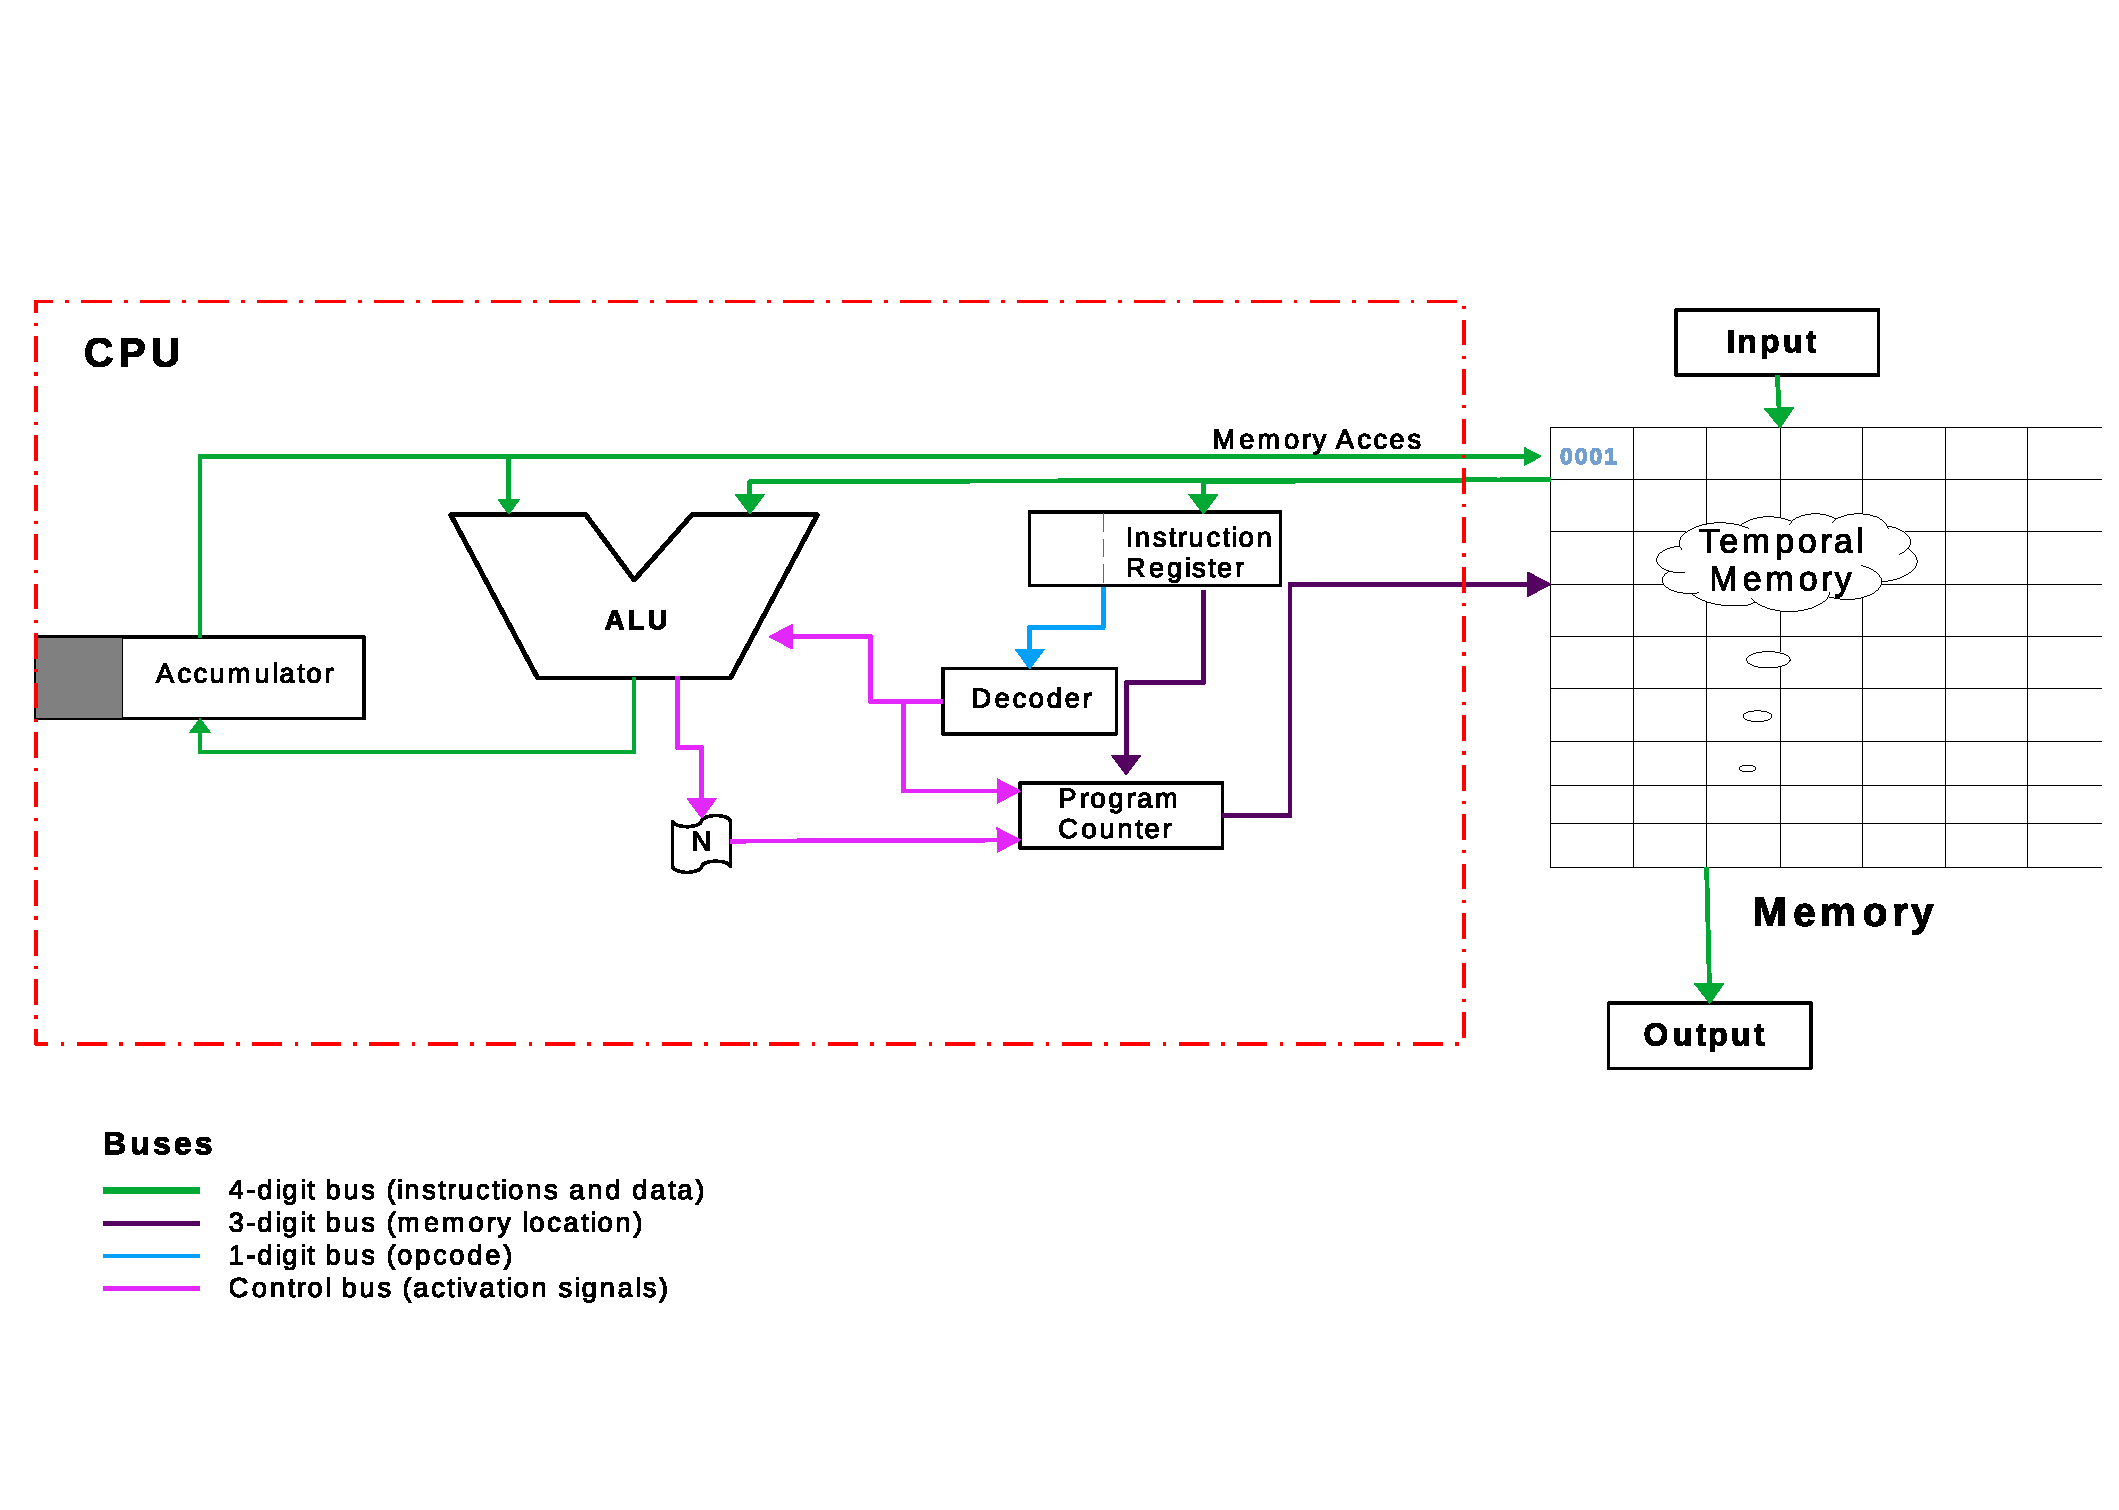
\includegraphics[scale=0.5]{media/CARDIACC/Arquitectura_diagrama_original.eps}
			\caption{Arquitectura de CARDIAC, concepto original Bell Labs \& Jorge Vasconcelos}
			\label{fig:Arquitectura_diagrama_original}
	\end{figure}
	
	
	
	La \textit{CPU}, es la unidad dónde se concentran todos los elementos que hacen 
	posible el cómputo de las instrucciones y datos
	que se almacenan en la memoria principal.
	Está conformada por los elementos que están dentro de la línea punteada en rojo en la imagen
	 \ref{fig:Arq_CARDIAC}. Por la importancia
	de cada elemento dentro de la unidad de procesamiento central (\textit{Central Processing Unit}),
	se hará un repaso individual a cada uno.
	
	Revisaremos cada elemento de la \textit{CPU} analizando sus funciones, para ello,
	es preciso tener claro el concepto de \textbf{ciclo}, el cual podemos entender vagamente 
	como la situación en la que regresas a la posición inicial una y otra vez. Un ciclo, empieza
	cuando el \textit{Program Counter}, o contador de programa, apunta hacía una dirección, 
	la primera sería la \#00; continua,
	cuando la CPU toma el contenido de esa dirección y por medio del bus verde la transporta hacía el 
	registro de instrucciones, que se encarga de separar el dígito a extrema izquierda \textit{d2}
	para enviarlo al decodificador
	por medio de un bus azul, y que este lo decodifique
	para transmitirle esa instrucción a la 
	unidad aritmético lógica. Cuando el contador de programa salte a otra dirección de memoria, 
	se habrá temrinado un ciclo y
	empezará otro \cite{fingerman_instruction_1968}. 
 
    Por otra parte, el mismo registro de instrucciones transfiere al contador de programa 
	los dígitos \textit{d1} y \textit{d2},
	por si este los ocupa para saltar a una dirección específica. Si los ocupa, el decodificador 
	le envia una señal, por medio 
	del bus rosa, que le indica saltar a una dirección particular \cite{fingerman_instruction_1968}.
	
	Continuando con la \textit{ALU}, esta realiza el cálculo que le indica el código de operación.
	Si el resultado que va a guardar
	en el acumulador es negativo, manda una señal a \textit{Negativo (N)},
	una especie de booleano que indica si un número 
	que ha sido depositado en el acumulador es
	o no negativo. Lo último que realiza la \textit{ALU} es almacenar el resultado de la operación
	en el  acumulador, un único registro
	que tiene la capacidad de almacenar solo cuatro dígitos (uno más que la memoria principal), 
	y es donde se almacenarán todos
	los cómputos que realice la \textit{ALU} \cite{fingerman_instruction_1968}. 
	
	En caso de que la unidad aritmética requiera información
	de la memoria  para ejecutar una instrucción,
	la puede recuperar directamente por medio de los buses verdes. Dado que, si se requiere información
	de la memoria, significa que la instrucción así lo indicaba,
	y por lo tanto, los dígitos \textit{d1} y \textit{d0}, del dato recogido por el registro
	de instrucciones,
	tienen la dirección de dónde se debe recuperar.  Únicamente
	si la \textit{ALU} obtiene el contenido de una dirección de esta forma, es que este
	será tratado como dato y no como instrucción. Si el contador de programa apunta a cualquier
	lugar de la memoria, el contenido de ese espacio será tratado como instrucción, a pesar
	de que no lo sea, lo que pude causar inconsistencias si no se es lo suficientemente
	 cuidadoso al escribir \cite{fingerman_instruction_1968}.
	
	De esta forma terminamos un ciclo cuando el contador de programa salta,
	 que puede ser porque una instrucción se lo indique, o bien porque
	la \textit{ALU} termino sus cómputos y entonces el contador de programa puede continuar
	 a la siguiente dirección de forma incremental
	sin algún cambio \cite{fingerman_instruction_1968}.
	
	Los periféricos también juegan un papel importante, aunque solo se conectan
	directamente a la memoria principal. Si se requiere imprimir algún resultado que este
	en el acumulador, este debe ser enviado primero
	a la memoria principal, para que se pueda realizar posteriormente 
	la operación de impresión de un espacio de la memoria principal 
	\cite{fingerman_instruction_1968}.
	
	%%
	\subsection{Funcionamiento y lenguaje en CARDIAC}	
	
	Ahora conocemos los elementos de este modelo y como interactúan, pero lo visitamos de cierta forma ``a ciegas'', no conocemos el lenguaje
	que utiliza esta ``máquina'', y como mencionamos antes, tanto la máquina hace al lenguaje como el lenguaje a la máquina. En la tabla \ref{tab:simple-table} podemos ver el lenguaje que se usa en código máquina(Código de operación), y 
	en 	ensamblador(Mnemotecnia) para CARDIAC, que es mucho más fácil de entender. Analizaremos cada una de las instrucciones presentadas
	originalmente en \cite{fingerman_instruction_1968} para entender la razón de su 
	existencia.
	
	
	\begin{table}[h]
	  \centering
	  \begin{tabular}{|c|c|p{8cm}|}
	    \hline
    	\textbf{Código de operación} & \textbf{Mnemotecnia} & \textbf{Definición} \\
	    \hline
	    0 & INP & (INPUT) Guardar dato en memoria.\\
	    \hline
		1 & LDA & (LOAD)  Cargar en el acumulador información de la memoria.\\
		\hline
	    2 & ADD & (ADD)  Sumar al contenido del acumulador contenido en la memoria.\\
	    \hline
	    3 & BLZ & (Branch if Less than Zero) Saltar si la información en el acumulador es menor que cero.\\
	    \hline
	    4 & SHF & (SHIFT) Mover de izquierda y/o derecha el contenido del acumulador.\\
	    \hline
	    5 & OUT & (OUTPUT) Escribir en la salida el contenido de la memoria.\\
	    \hline
	    6 & STO & (STORE) Guardar información del acumulador en la memoria.\\
	    \hline
	    7 & SUB & (SUBSTRACT) Restar información de la memoria al acumulador.\\
	    \hline
	    8 & JMP & (JUMP) Saltar y guardar el valor del contador de programa en la dirección \#99. \\
	    \hline
	    9 & HLT & (HALT) Detener la ejecución del programa y reiniciar el contador del programa.\\
	    \hline
	  \end{tabular}
	  \caption{Lenguaje de programación de \textit{CARDIAC}.}
	  \label{tab:simple-table}
	\end{table}
	
	Para empezar necesitamos establecer una conexión entre el usuario y la máquina, que el usuario a través del dispositivo de entrada pueda
	darle información, con el código \textit{INP} podemos indicar el ingreso de información a la memoria principal. Con la instrucción  	
	\textit{012} estamos indicando que se guarde el dato que ingresa el usuario a través del dispositivo
	de entrada en la dirección de memoria \#12, notaremos que en 9 de las 10 instrucciones los últimos dos dígitos hacen referencia a la dirección.
 
	Posteriormente, necesitamos llevar información de la memoria al acumulador para realizar operaciones sobre ella, esto lo realizamos con el código 
	\textit{LDA}, por lo tanto, con la instrucción
	\textit{112} indicamos que se cargue en el acumulador la información almacenada en la dirección de memoria \#12.
 
    Supongamos que el valor
	que ingresamos, y que fue guardado en 
	\#12, es \textit{005}, entonces \textit{005} será cargado en el acumulador. Ahora, si lo que queremos es incrementar el valor
	del acumulador en una unidad podemos usar el contenido de la dirección \#00, dónde se encuentra el dato \textit{001},
	mismo que podemos utilizar en la instrucción \textit{ADD} de la siguiente forma: \textit{200}, que indica que hay que sumar el contenido de la 
	dirección \#00 a lo que tiene
	el acumulador, obteniendo un \textit{006} en el acumulador.
	
	\begin{table}[h]
	  \centering
	  \begin{tabular}{|c|c|c|c|}
	    \hline
    	\textbf{Dirección \#} & \textbf{Código máquina} & \textbf{Ensamblador} & \textbf{Estatus acumulador} \\
	    \hline
	     20 & 012 & INP 12 & 000 \\
	     21 & 112 & LDA 12 & 005\\
	     22 & 200 & ADD 00 & 006\\
	     23 & 712 & SUB 12 & 001\\
	     24 & 712 & SUB 12 & -004\\
	     25 & 200 & ADD 00 & -003\\
	     26 & 325 & BLZ 25 & 000\\
	     27 & 200 & ADD 00 & 001\\
	     28 & 880 & JMP 80 & 001\\
	     29 & 212 & ADD 12 & 012\\
	     30 & 432 & SHF 21 & 020\\
	     31 & 613 & STO 13 & 020\\
	     32 & 513 & OUT 13 & 020\\
	     33 & 900 & HLT 00 & 020\\
	    \hline
	  \end{tabular}
	  \caption{Programa principal (In-Util). }
	  \label{tab:Programa_Principal}
	\end{table}
	
	Para seguir analizando los códigos de operación disponibles tenemos un código en la tabla \ref{tab:Programa_Principal}, dónde
	podremos visualizar los códigos, su equivalente en ensamblador y como afectan al acumulador. Esté programa empieza en la
	dirección \#20, si nos damos cuenta las primeras tres instrucciones son las que revisamos en el párrafo anterior, y el
	estatus del acumulador expresa precisamente el valor que se mencionaba, el \textit{006}.

	Estamos ubicados en la dirección \#22, dónde nos moveremos a la \#23 en la que ocuparemos la instrucción de \textit{SUB} para restar, restaremos el 
	número que cargamos en la dirección \#12 a lo que tenemos en el acumulador, de hecho lo haremos dos veces seguidas para conseguir un número 	
	negativo, él \textit{-004}, si lo viésemos en operaciones matemáticas la operación sería la siguiente: $ 6-5-5 = -4 $.
 
    Los números negativos en este modelo son especiales, 
	como se habrá observado coloque el signo
	justo a la extrema izquierda, esto es porque para simplicidad del modelo los números negativos
	o positivos ocupan el mismo espacio. El signo siempre estará más a la izquierda que cualquier otro dígito, como las direcciones
	no pueden ser negativas no nos podemos encontrar con un caso del estilo \textit{1-42}. De modo
	parecido, el modelo se toma la libertad de tomar al cero como positivo, situación que será importante con las siguientes instrucciones.
	
	Nos	movemos a la dirección \#25, en la que se suma un uno al acumulador, y en la dirección \#26 ocupamos el código 
	\textit{BLZ} en la instrucción \textit{325} para obtener un salto condicional. Es decir, si el contenido del acumulador es menor a cero salta a la 
	dirección \#25, por lo que se formara
	un bucle en el que el acumulador cambiara de valor de uno en uno hasta llegar a cero después de cuatro vueltas, momento en el que el condicional 
	dejara avanzar al contador de programa a la siguiente instrucción y no forzando el salto a \#25, pues, el valor del acumulador ya es
	positivo(para los fines del modelo).
	
	
	Lo que sigue es ver el funcionamiento de la operación \textit{JMP}, para esto continuamos con la ejecución, vemos que en la dirección
	\#27 se le suma un uno al acumulador para tener en el acumulador un \textit{001}. Posteriormente está la operación
	de salto, que realiza uno a
	la dirección \#80, dónde se encuentra
	una \textbf{subrutina}, un programa ``pequeño'' generalmente usado por otros para reproducir un resultado.
 
    En este caso lo que hace
	es sumar un seis a lo que tenga el acumulador cuando el programa origen salte. Como nosotros tenemos un
	uno en el acumulador y queremos sumarle seis, la forma más fácil de hacerlo es saltando a esa subrutina que regresara a la dirección
	siguiente cuando termine, la \#29.
	
	Esté funcionamiento lo podemos lograr fácilmente debido a que la instrucción \textit{JMP} al momento de saltar guarda la 
	dirección de memoria de la cual salta en la dirección \#99, con el sufijo \textit{8}. Si miramos la tabla \ref{tab:subrutina}, dónde se encuentra
	está subrutina, notaremos que lo primero que hace es cargar en el acumulador el contenido de la dirección \#99, que en
	esté caso es un \textit{828}, pues salto desde la dirección \#28, posterior se le suma un uno
	para así tener la dirección \#29, que es a la que tiene  que regresar la subrutina cuando termine. Para lograrlo, en la dirección
	\#82 indica que se guarde el resultado del acumulador en la última dirección de la subrutina, así cuando terminen todas las adiciones
	saltará a la dirección \#29.
	
	Como apunte importante, si leyeron el manual
	de \textit{CARDIAC} se habrán dado cuenta de que hay una ligera diferencia con la instrucción \textit{JMP}, pues en el manual dice que guarda la dirección
	de la que salto más uno, es decir, si salto de la dirección \#28 lo que se guardará en \#99 será la dirección \#29, un \textit{829}. Lo que en nuestro
	ejemplo particular ahorraría código, pero por los usos que se le dará en los siguientes modelos decidí que sería más eficiente como la he definido en esta sección, y esto
	es porque se tiene más precisión al tener la información más pura de dónde salto el programa. Y por supuesto, ambas definiciones pueden llegar a los
	mismos resultados con algunos cambios en la codificación.
	
	\begin{table}[h]
	  \centering
	  \begin{tabular}{|c|c|c|c|}
	    \hline
    	\textbf{Dirección \#} & \textbf{Código máquina} & \textbf{Ensamblador} & \textbf{Estatus acumulador} \\
	    \hline
	     80 & 199 & LDA 99 & 828 \\
	     81 & 200 & ADD 00 & 829 \\
	     82 & 690 & STO 90 & 829 \\
	     83 & 100 & LDA 00 & 001 \\
	     84 & 200 & ADD 00 & 002 \\
	     85 & 200 & ADD 00 & 003 \\
	     86 & 200 & ADD 00 & 004 \\
	     87 & 200 & ADD 00 & 005 \\
	     88 & 200 & ADD 00 & 006 \\
	     89 & 200 & ADD 00 & 007 \\
	     90 & 829 & JMP 29 & 007 \\
	    \hline
	  \end{tabular}
	  \caption{Subrutina para sumar varios unos.}
	  \label{tab:subrutina}
	\end{table}
	
	
	Continuando con el programa principal de la tabla \ref{tab:Programa_Principal}, y habiendo regresado de la subrutina en
	la dirección \#29 con
	un valor en el acumulador de \textit{006}, la operación que se
 realiza en esa dirección es una suma para dejar
 el valor del acumulador en \textit{012}, valor que será muy
	interesante para analizar el siguiente código de operación, \textit{shift/SHF}.
 
    Deje esté código para  casi el final 	
	por qué
	es la menos intuitiva, no es una de las operaciones básicas que usualmente tenemos en mente; sin embargo, cumple un papel fundamental, en las 
	computadoras binarias cumple un papel aún más crucial por las operaciones entre bits que se pueden realizar, pero en una decimal
	también aporta mucha flexibilidad y eficiencia en el uso de memoria para una gran variedad de operaciones.
	
	En la dirección \#30 vemos que el efecto de aplicar esta operación con la instrucción \textit{432} cambia el número \textit{012} por
	el \textit{020}. Esto sucede por qué el dígito \textit{d1} indica cuantos lugares a la izquierda se desplazará el valor
	del acumulador, dejando en 0 los espacios vacíos, mientras que el dígito \textit{d0} indica cuantos lugares a la derecha se desplazará.
	Aquí será muy importante la consideración especial de espacio que tiene el acumulador respecto a las celdas de la memoria principal, pues
	para evitar el desbordamiento accidental el acumulador siempre tendrá \textbf{un dígito más} del que las celdas de la memoria principal tengan,
	en este caso el acumulador puede almacenar hasta 4 dígitos.
	
	Si consideramos lo anterior y vemos la instrucción \textit{432}, lo que nos indica primero es mover tres lugares a la izquierda
	el valor del acumulador, $0012$, dando como resultado $2000$, pues el \textit{1} queda fuera
	del espacio del acumulador, por lo que este número se pierde para siempre y no se podrá recuperar. Si le aplicamos el desplazamiento de dos lugares 	
	a la derecha que se nos indica, terminaremos con $0020$ en el acumulador, como podemos ver el \textit{1} se perdió, y aunque desplacemos
	en el sentido contrario, si este ya se quedó fuera del espacio del acumulador no podrá regresar. Para simplificar y como prácticamente no se usa el cuarto dígito dejamos indicado el resultado solo como $020$ en la tabla \ref{tab:Programa_Principal}.
	
	
	Para persistir los datos  en \#31 tenemos la instrucción para guardar la información del acumulador(\textit{STO}) en la dirección de memoria número
	\#13. Posteriormente, con el código  \textit{OUT} se establece la conexión con el dispositivo de salida para exportar los resultados
	que se guardaron en \#13, debido a que la instrucción \textit{513} indica con sus últimos dos dígitos la dirección
	de memoria de la cual se tomará la información.
 
    Finalmente, el programa se termina con el código  \textit{HLT}, marcando el
	final del programa y se reinicia el contador del programa
	a la dirección \#00, pues es lo que se indica con los dígitos \textit{d1} y \textit{d0} de la instrucción \textit{900}. Después de este repaso podemos constatar que en casi todos los códigos de operación los dígitos \textit{d1} y \textit{d0} hacen
	referencia a una dirección de memoria, salvo por \textit{SHF} en la cual tienen un funcionamiento especial.
	
	Con este lenguaje, simple, pero eficaz, podemos construir cualquier programa que queramos,
	puesto al tener ciclos, condicionales y la posibilidad de realizar
	las operaciones aritméticas básicas (suma y resta), podemos
	decir que es Turing completo, por lo que nuestra única limitante es la memoria.
	
	
	

	\clearpage	
	
\chapter{Evolución del Modelo}  %

	Como pudimos ver en los capítulos anteriores, CARDIAC es sumamente útil para explicar aspectos importantes de la computación y el cómo se organizan sus 	
	componentes; sin embargo, no podemos negar que a día de hoy es un tanto insuficiente para explicar las computadoras más modernas que tienen
	una concurrencia y un paralelismo sin los cuales no entenderíamos a las computadoras. No podemos imaginar una computadora en la cual no podamos 	
	ejecutar más de un proceso a la vez, por ello una evolución del modelo creado en los años 60 por \cite{fingerman_instruction_1968} es
	necesaria. Pero ello implica diferentes retos, retos que se abordarán en este capítulo.
	
	Pero no solo en el apartado de diseño y organización del modelo se tendrá una actualización, sino también en la forma de presentarlo. Aprovechando
	las facilidades de algunos lenguajes de programación, he realizado una simulación en Java para mostrar las mejoras realizadas al modelo
	original y que sea más sencillo mostrar la interacción de los distintos componentes de una computadora.
 
    La idea detrás de esta simulación
	no es solo emular los comportamientos de CARDIAC en una computadora actual para ejecutar algunos programas,
	sino realmente realizar una \textbf{máquina virtual}, es decir, un software que represente
	el modelo, tanto a nivel hardware como a nivel software, de manera virtual.
 
    En la imagen \ref{fig:welcomeec} tenemos la pantalla de inicio
	dónde se puede seleccionar la máquina virtual que queremos probar. Como se podrá notar, he agregado la \textit{E}(de electrónico) que vemos tanto últimamente, como sufijo de las tres máquinas virtuales para resaltar su aspecto
	electrónico distante del que tenía en los años 60. 


	
	\begin{figure}[h]
 			\centering
			\includegraphics[scale=0.5]{media/CARDIACC/WelcomeEC.png}
			\caption{Inicio para selección de máquinas virtuales}
			\label{fig:welcomeec}
	\end{figure}

	\clearpage
	\section{E-CARDIAC : Electronic CARDboard Illustrative Aid to Computation}
	
	Después de entrar al software de simulación y ver la pantalla de bienvenida, como se ve en la figura \ref{fig:welcomeec}, lo que sigue es elegir la máquina
	que queremos probar. En este caso comenzaremos con la versión que es prácticamente el modelo original
	llevado a un software de simulación.En términos
	generales, las tres máquinas tendrán un esqueleto similar, por lo que una vez que conozcamos el funcionamiento de esta primera, será muy sencillo
	entender el funcionamiento de las otras dos, aunque estás tengan más componentes.
 
    Para empezar será bueno visualizar el diagrama de la arquitectura de CARDIAC, diagrama 
	que se puede apreciar en la figura \ref{fig:arqCardiac}, y que se irá comentando de acuerdo a los componentes a los que se haga referencia. Pero
	como observación general se puede apreciar la CPU a la izquierda, la memoria a la derecha con una descripción de cómo son sus dígitos, y en la parte
	inferior las diferencias entre los buses que la componen, así como el contenido de las celdas con información predefinida.

    \subsubsection{Configuración de la máquina virtual}
    
	\begin{figure}[h]
 			\centering
			\includegraphics[scale=0.5]{media/ECARDIAC/arq_cardiac.png}
			\caption{Arquitectura de CARDIAC por Jorge Vasconcelos, 2018}
			\label{fig:arqCardiac}
	\end{figure}	
	
	En la figura \ref{fig:iniECardiac} podemos ver el esqueleto de lo que será nuestra máquina, que aún se encuentra apagada, porque al entrar
	lo que nos encontramos es una máquina apagada, que podemos encender al dar clic sobre el botón \textit{start}. Pero antes de dar clic ahí podemos
	ver que en esa barra principal tenemos varias opciones, a extrema izquierda está un símbolo de casa y un botón que dice \textit{CARDIAC Systems}, que
	nos permitirá regresar a la página de inicio si así lo deseamos.
 
    Continuando en el centro tenemos tres botones, el que ya vimos para encenderla, otro para pausarla, algo poco común en una máquina de verdad, pero bastante usual en los software de máquinas virtuales. El uso de este botón de pausa
	nos permite detener el funcionamiento completo sin afectar los procesos internos, analizar su estado
	y después continuar como si nada hubiera pasado; por último, el tercer botón es para reiniciarla.
	
	En la
	parte derecha de la misma imagen podemos ver dos casillas, una con un 100 y la otra con la palabra ``Normal''. Estas son dos listas desplegables, la primera permite 
	elegir la cantidad de celdas con las que la máquina funcionara, es decir, la memoria disponible, y la segunda es para elegir la velocidad de la máquina. De esa
	forma podemos decidir cuanto va a tardar cada ciclo en ser completado con el fin de observar su comportamiento.
 
    En la figura \ref{fig:listasDespCardiac}
	podemos ver las listas desplegadas con las opciones que tienen disponibles, como podemos ver hay distintas velocidades; para ver con más detalle el proceso
	está \textit{slow}, o si queremos el resultado de inmediato está la opción \textit{instant}. En el caso de la memoria, el funcionamiento es más interesante, pues
	no es solo una configuración externa a la máquina, sino que afecta directamente a la arquitectura y al lenguaje, puesto que con 1000 celdas el lenguaje
	debe cambiar para recibir direcciones de 3 dígitos. Aunque el cambio en el lenguaje sería solo ese, por lo demás solo sería la adaptación, mismo
	caso que para 10,000 celdas. Al elegir la cantidad de memoria y luego encender la máquina, esta se configura en su arquitectura para trabajar con esa
	cantidad de memoria y recibir instrucciones con direcciones más grandes.

	\begin{figure}[h]
 			\centering
			\includegraphics[scale=0.4]{media/ECARDIAC/ECARDIAC_P1.png}
			\caption{Pantalla de inicio de E-CARDIAC}
			\label{fig:iniECardiac}
	\end{figure}


	\begin{figure}[H]
 			\centering
			\includegraphics[scale=0.45]{media/ECARDIAC/ecardiac_lista_velocidad.png}
			\caption{Listas desplegables de E-CARDIAC}
			\label{fig:listasDespCardiac}
	\end{figure}

	
    \subsubsection{Unidad central de procesamiento}
    
	Continuando con los elementos que tiene la máquina virtual, podemos ver en la parte izquierda de la figura \ref{fig:iniECardiac}  cuatro secciones; los
	componentes principales de la máquina en la
	\textit{Central Processing Unit(CPU)}, el estado de la máquina en la parte del \textit{machinne status(estado de la máquina)}, un apartado para las salidas en el \textit{output}, y un apartado en 
	blanco(\textit{queue}), que servirá como cola de espera para la ejecución de las instrucciones.
 
    En la primer sección, que es la \textit{CPU}, podemos notar que está el
	registro de instrucciones(\textit{instruction register}), que contendrá la instrucción que viaja a través del bus verde desde la memoria a la \textit{CPU}. Después el 
	código de operación(\textit{Operational Code}) y el operando(\textit{Operand}), que son los resultados que presenta el decodificador, en la figura
	\ref{fig:arqCardiac}), después de que una instrucción pasa por él.
 
    Posterior se encuentra el contador de programa (\textit{Program Counter}), el componente que se 
	encarga de hacer avanzar la lectura de instrucciones sobre la memoria. El número que contenga el contador de programa es la dirección en la que se encuentra
	el ``puntero'' de la máquina, es decir que el contenido de tal dirección que es ``apuntada'' por el contador será transmitido a la \textit{CPU}.
 
    Más abajo se
	encuentra el acumulador(\textit{Acumulator}) y la bandera para saber si un número es negativo(\textit{Negative}). El acumulador contendrá los resultados que arroje
	la unidad aritmético-lógica(\textit{ALU} en diagrama de CARDIAC), o bien algún valor que sea cargado directamente desde memoria por alguna instrucción como \textit{LDA}.                                                                                                                                                                                                                                                                                      \subsubsection{Estado de la máquina y dispositivo de salida}                                         
	
	En la sección \textit{Machinne Status}, tenemos elementos externos a la arquitectura de la computadora. Estos nos definen el
	estado de la máquina en cada momento, en cada ciclo que pasa nos indica directamente si la máquina está funcionando correctamente (\textit{CARDIAC is working}),
	pausada(\textit{CARDIAC is paused}) o si, por el contrario, dejo de funcionar(\textit{CARDIAC is dead}). Esté último puede ser causado por diversas razones
	que hagan CARDIAC realice operaciones indebidas, como pasar un negativo como instrucción, para lo cual no tiene respuesta
	y lo único que hará es detenerse. 
 
    También en esta sección está un apartado que indica la operación que estará ejecutando la \textit{CPU}, \textit{Operation}, y el ciclo en el que se encuentra con \textit{Cycle}.

  
 
	La tercera sección muestra la salida en forma de lista, como podemos ver en la figura \ref{fig:ecardiacOutput}, emulando lo que eran las salidas de las primeras 
	computadoras que podían imprimir resultados
	en cintas perforadas. En esta misma sección está un apartado para ``descargar'' la cinta y guardarla
	como un archivo de texto, que por defecto se guarda en la carpeta de descargas.

	\begin{figure}[h]
 			\centering
			\includegraphics[scale=0.27]{media/ECARDIAC/OutputFullfilled.png}
			\caption{E-CARDIAC Muestra de Output}
			\label{fig:ecardiacOutput}
	\end{figure}

    \subsubsection{Entrada de datos e instrucciones}
 
	Toda la parte inferior está relacionada, puesto que en la izquierda está la lista de instrucciones en cola por ser leídas(en \textit{Queue}),
	como en la figura \ref{fig:ecardiacQueue} se muestra. Estas instrucciones,
	el usuario podrá añadirlas a la cola desde la pestaña \textit{Deck Mode(modo tarjeta)}, se podrán cargar desde ahí con solo escribirlas
	en forma de lista y dar clic en agregar tarjeta(\textit{Add Card}), como se ve en la figura \ref{fig:ecardiacDeckMode}, dónde podemos ver una
	lista de instrucciones previo a ser añadidas a la cola.
 
    Por otra parte, si se desea añadir instrucciones/datos de forma individual, uno a uno, se cuenta
	con la otra pestaña que dice \textit{Terminal Mode(modo terminal)},  del cual podemos ver un ejemplo de la carga en la figura \ref{fig:ecardiacTerminalMode}. Pero para hacer uso
	de esta pestaña es necesario que exista una instrucción que indique, como en el ejemplo,  que se espera una entrada en una celda, en caso contrario
	no se permitirá agregar datos de esa manera. Debido a que este modo transfiere directo los datos o instrucciones a la memoria en la posición solicitada,
	a diferencia del modo de tarjetas, que siempre primero las manda a la cola de espera, que las hará pasar posteriormente, cuando se solicite,
	a la memoria principal.


	\begin{figure}[h]
 			\centering
			\includegraphics[scale=0.4]{media/ECARDIAC/DeckModeLoaded.png}
			\caption{E-CARDIAC Carga masiva por tarjetas}
			\label{fig:ecardiacDeckMode}
	\end{figure}
	
	\begin{figure}[h]
 			\centering
			\includegraphics[scale=0.25]{media/ECARDIAC/TerminalMode.png}
			\caption{E-CARDIAC Carga individual de instrucciones}
			\label{fig:ecardiacTerminalMode}
	\end{figure}
	
	\begin{figure}[H]
 			\centering
			\includegraphics[scale=0.4]{media/ECARDIAC/QueueCargada.png}
			\caption{E-CARDIAC Cola de instrucciones/datos}
			\label{fig:ecardiacQueue}
	\end{figure}		

 \subsubsection{Encendiendo E-CARDIAC}

	En varias de las imágenes mencionadas en párrafos anteriores se mostró cómo se ve la memoria principal, pero veamos ahora la figura \ref{fig:enceCardiac} para
	ver la máquina cuando acaba de encender y centrémonos en la memoria principal, compuesta de 100 celdas numeradas del \#00 al \#99 con los datos
	por defecto que tienen en esas especies de memorias ROM. En color blanco con fondo gris están todas las direcciones de memoria, y con un fondo blanco, pero
	contenido en negro, los datos que contiene cada dirección. Para diferenciar la dirección de la celda de la cual el contenido está siendo transmitido
	a la \textit{CPU} se tiene el color azul marino, en el caso del ejemplo nos indica que se está leyendo la instrucción en la dirección \#00.
	

	\begin{figure}[H]
			\includegraphics[scale=0.28]{media/ECARDIAC/ECARDIAC_P2.png}
			\caption{E-CARDIAC después de iniciar sus funciones}
			\label{fig:enceCardiac}
			
	\end{figure}
	
	
	De esta forma terminamos el recorrido por la máquina virtual de \textbf{E-CARDIAC}, que nos permitirá experimentar con más soltura la programación en
	lenguaje ensamblador. La siguiente evolución del modelo requerirá de un aumento en la memoria de CARDIAC, que es muy fácil
	de aplicar sobre esta  máquina virtual como ya lo hemos visto, y que podremos estudiar con más profundidad en la siguiente
	sección.


	\clearpage	
		
	\section{E-CARDIAC C : Electronic CARDboard Illustrative Aid to Concurrent Computing}
		
	El nombre es un homenaje al lenguaje de programación \textbf{C}, agregando esa ``C'' al final del nombre que tenía el modelo anterior
	para expresar que la diferencia entre estos dos es la concurrencia. \textit{E-CARIDAC C}, ayuda ilustrativa de cartón electrónico para
	la computación concurrente, por sus siglas en inglés, tiene la intención de ser un modelo que represente la organización de una computadora que puede tener operaciones concurrentes
	y poder ver cómo interactúan las distintas partes de la computadora para lograr la concurrencia.
 
    Buscamos la concurrencia a nivel procesos
	en este caso, dado que generalmente es utilizada en las computadoras comunes. Esto nos lleva a tener que hacer varios cambios en el diseño original
	del modelo, agregar mecanismos en el Hardware, en el Software y diseñar una especie de sistema operativo para poder lograr la concurrencia de 
	procesos.
	

	
	
		\subsection{Necesidad de un sistema operativo}
		
		El primer paso es entender la necesidad de tener un sistema que administre los recursos de la máquina, sin ello podemos construir muchos programas, pero
		la ejecución deberá ser individual a nuestra disposición, de cierta manera seríamos nosotros mismos ese sistema de administración. En 
		\cite[p. 42]{fingerman_instruction_1968}
		nos presentan un sistema de carga de programas para el modelo original, un cargador(\textit{bootloader}), diseñado para poder escribir en ``tarjetas'' un programa, y que se vaya
		añadiendo a la memoria de CARDIAC sin la necesidad de literalmente colocar en los espacios de memoria de CARDIAC las instrucciones, pero esto aún nos deja
		con la tarea de decidir que programa va primero.
  
        Así que partiendo de este punto podemos concluir que el programa que realice esa tarea será un\textbf{ sistema
		operativo mínimo}, y necesita el sufijo de mínimo, por qué la otra característica que define
		a un sistema operativo es ser una capa de abstracción entre la máquina y otros programas. En este
		caso, el sistema operativo que se diseñará no tiene la intención de ser una capa de abstracción tan marcada, tendrá algunos aspectos que pueden ser considerados
		una capa de abstracción entre los programas y la máquina, pero no lo será completamente. Por tal razón lo nombraremos como sistema operativo mínimo o \textit{SOM} en el resto del texto.
		
		Entendiendo un programa que realice tal tarea parece evidente que el espacio de memoria del modelo original será insuficiente, por lo que una de las necesidades
		derivadas del SOM será la ampliación de la memoria, lo que llevará a un cambio también en el lenguaje que es diseñado específicamente para direcciones de dos 
		dígitos.
  
        Y seguramente la implementación de un sistema operativo requerirá de algún sistema de almacenamiento secundario para el programa, de forma que no esté
		cargado directamente en la memoria principal como si de una memoria ROM se tratara. Esto derivaría en la necesidad de conectar ese almacenamiento secundario
		con la memoria principal y por ende aumentar la cantidad de buses.
  
        Además, al ser un programa que requiera unos privilegios de control de la máquina más elevados,
		quizá se necesiten piezas de hardware que en su versión original CARDIAC no necesitaba.
		
		\subsection{Mejoras necesarias en el Hardware}
		
		Para solucionar las necesidades mencionadas más arriba decidí aumentar las celdas de memoria de 100 a 1000, de forma que cada dirección posible tendrá
		tres dígitos, así un número completo de cuatro dígitos puede representar tanto el número en sí mismo, como un código de operación acompañado de tres operandos.
  
        Por lo tanto, los buses deberán ser capaces de transmitir más dígitos que en el modelo original, en la figura \ref{fig:diagarquiConc} 
		podemos observar
		en la parte inferior izquierda como serán los buses; los de color verde, que son los de mayor capacidad, transmitirán instrucciones y datos, los
		que están en color morado solo las direcciones, mientras que los que están en color azul solo los códigos de operación. Adicionalmente, hay unos buses
		en color rosa que transmitirán señales de activación.
  
        En la misma imagen se puede apreciar que al principio y al final de la memoria las celdas no han cambiado
		mucho, al principio está un valor que será inmutable que tiene el mismo significado que en el modelo original, salvo que con un cero extra por el crecimiento
		en el tamaño de la memoria. La misma situación la tiene el valor del final de la memoria, que solo podrá contener valores que inicien con un $8$, y
		que por defecto será $8000$. El sufijo que sigue al código de operación $8$ será la dirección de memoria de dónde se tomó una instrucción de salto 
		que fue ejecutada.
				
		\begin{figure}[h]		
			\centering
			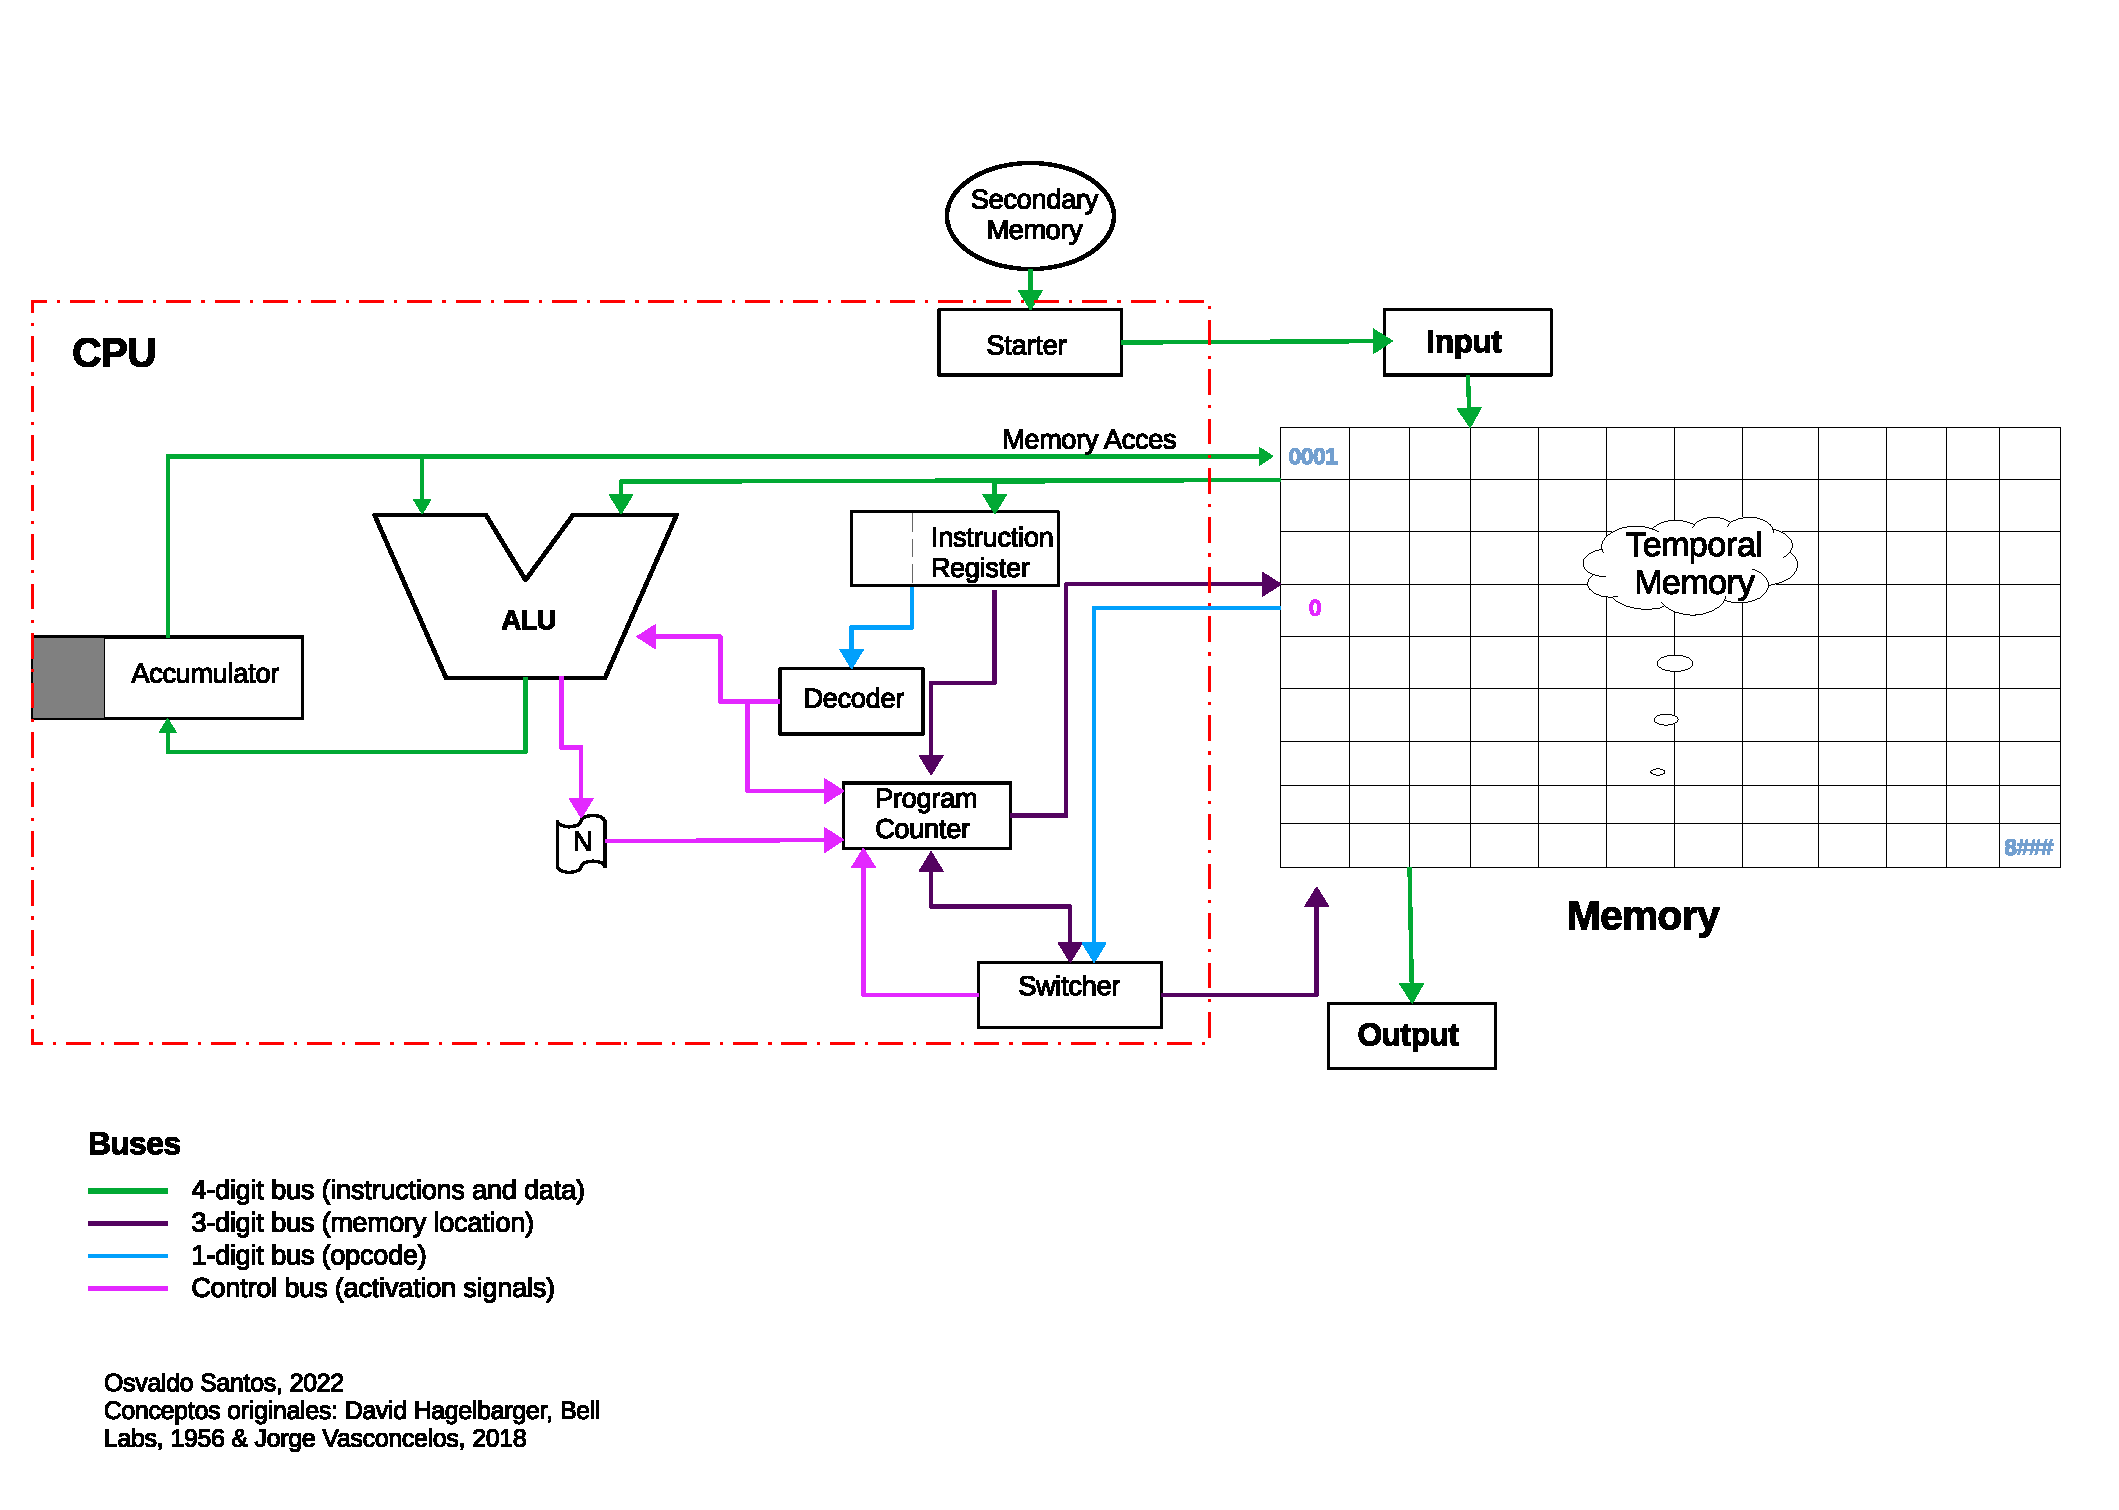
\includegraphics[scale=0.5]{media/CARDIACC/Arquitectura_diagrama_concurrente.eps}
			\caption{Diagrama de Arquitectura de E-CARDIAC C}
			\label{fig:diagarquiConc}
		\end{figure}
		
		
		Esto permite mantener varios elementos del funcionamiento del modelo original sin cambios, pero podemos notar tres de elementos nuevos, que a su vez
		incrementan el número de buses presentes en el modelo. Analicemos primero al que está conectado con el dispositivo de entrada(\textit{input}), en la parte superior del centro,
		el que tiene por nombre \textbf{starter}(iniciador), y que a su vez está conectado con otro elemento nuevo llamado \textbf{secondary memory}(memoria secundaria).

  
		La memoria secundaria es la representación de lo que vendría siendo el disco duro en las computadoras, pero más limitada por qué solo sería de un almacenamiento
		muy puntual para el sistema operativo. Siendo una especie de tarjeta con un programa específico, que
		está conectada a través del iniciador para que apenas se inicie la máquina, lo primero que haga es empezar a agregar las instrucciones guardadas
		en la memoria secundaria a la pila de ejecución a través del dispositivo de entrada.
  
        De esta manera podemos mantener simple el modelo, pero establecer una conexión
		con otra fuente de información diferente a la memoria principal, y poder colocar el sistema operativo mínimo de una forma más natural sin que esté ahí como si fuera parte de la memoria ROM.
		
		
		El otro integrante de este nuevo modelo es el que tiene por nombre \textbf{switcher}(conmutador), que está en la parte inferior derecha del área del CPU.
		Este elemento es la solución al problema que tiene la inclusión de un programa que necesita tener los privilegios de poder tomar el control de las ejecuciones,
		cederlo a otros programas, y poder recuperarlo en un momento particular.
  
        Como se puede observar en la imagen, tiene 4 diferentes conexiones, siendo uno
		de los que más tiene. Su función radica en que cada \textbf{N} ciclos manda una señal(con el bus rosa) al contador de programa para que salte a la \textbf{dirección 
		de inicio del sistema operativo}, dirección que tiene que ser establecida en la configuración inicial de la misma arquitectura. Esto lo hace siempre y cuando en la dirección
		\#003 el valor que esté ahí sea $1$, que indica que es tiempo de ejecución del usuario y, por tanto, cada N ciclos los recursos regresan al SOM. Si
		el valor fuese un $0$, como es por defecto, no haría esos saltos, puesto que significa que los recursos los tiene el SOM, el cual puede disponer
		de ellos sin límite al tener todos los privilegios posibles. Esta conexión entre el conmutador y la memoria principal se hace con un bus que azul, pues solo requiere de un dígito.
  
        Otra conexión que tiene es una bidireccional al contador de programa, que le permite contar los ciclos que han sucedido desde que el SOM cedió el control e indicarle al contador de programa cuando debe regresar los recursos al SOM, y a qué dirección
		tiene que saltar cuando se trata de regresar el control de los recursos al SOM. El contador del \textit{conmutador} sigue al contador de programa, pero se reinicia cada que la bandera de saltos cambia de valor.
        Para todo esto se requiere un bus de color morado, para transmitir las direcciones y datos, y uno color rosa para mandar la señal al contador de programa de que debe interrumpir su proceso natural.
  
        Una razón adicional para esta conexión bidireccional es que el \textit{conmutador} recibe del contador programa la última dirección
		apuntada por el proceso del usuario, antes de que fuera ejecutada. Esto sucede debido a que para ese momento si se llegaron a los N ciclos se da la instrucción
		de regresar los recursos al SOM, y en ese momento la dirección es transmitida al \textit{conmutador}, para que este, por medio de su conexión a la memoria principal(por el bus morado),
		la coloque en una dirección especial para que el SOM pueda recuperarla. Para que después, cuando regrese los recursos a ese proceso, pueda continuar
		justo en la instrucción que ya no pudo ejecutar.
		
		El sistema operativo mínimo en su mismo proceso lanza los procesos del usuario, y por ende realiza los saltos necesarios para ceder los recursos. Pero antes de lanzarlos,		
		modifica el valor de la dirección $\#003$ a $1$, para que el \textit{conmutador} pueda regresar el control al SOM después de N ciclos aproximadamente.< Aclarando
		la parte de ``N ciclos aproximadamente'', es por qué
		una vez que es cambiado el valor a $1$ por el SOM en la dirección que funge como \textbf{bandera de saltos}, aún ejecutará un par de instrucciones propias
		del SOM para lanzar otros procesos, por lo que en realidad el proceso del usuario tendrá $N-2$ ciclos disponibles antes de regresar los recursos.
		
		Por supuesto, con todos estos cambios hechos para poder instalar un sistema que administre la ejecución de procesos concurrentemente, el lenguaje también
		requiere modificaciones, en su mayoría mínimas, pero otras que van orientadas totalmente a funcionar con un sistema operativo.
		
		\subsection{Cambios en el lenguaje}
		
		Como ya leímos en secciones pasadas, el lenguaje de una máquina muchas veces es consecuencia de las posibilidades que el hardware le provee. Pero
		también el lenguaje define ciertas necesidades del hardware, por lo que en la construcción de una computadora se necesita pensar en todos
		los elementos que van a interactuar juntos. 
  
        Para E-CARDIAC C agregamos un nivel extra, la consideración del sistema operativo mínimo, pues como
		podemos notar en la tabla \ref{tab:programing_language_ecc}, uno de los únicos dos cambios que hubo es en la instrucción \textit{halt}. Esta está diseñada ahora para funcionar con un sistema operativo, pues por sí sola no tendrá las capacidades completas, que sí tendrá con un SOM.
        
        En la configuración inicial de la computadora se definirá la dirección  establecida como \textit{área de borrado} para el SOM, área que ocupa la instrucción \textit{halt} para finalizar procesos. Con esto
		podemos considerar que nuestro SOM es, en cierto punto, una capa de abstracción entre el código máquina puro, y las instrucciones que usa el usuario en sus procesos.

		
		
			\begin{table}[h]
			  \centering
			  \begin{tabular}{|c|c|p{8cm}|}
			    \hline
		    	\textbf{Código de operación} & \textbf{Mnemotecnia} & \textbf{Definición} \\
			    \hline
			    0 & INP & Guardar datos en memoria.\\
			    \hline
				1 & LDA & Cargar en el acumulador información de la memoria.\\
				\hline
			    2 & ADD & Sumar al contenido del acumulador contenido en la memoria.\\
			    \hline
			    3 & BLZ & Saltar si la información en el acumulador es menor que cero.\\
			    \hline
			    4 & SHF & Mover d1 veces a la izquierda el número y d0 veces a la derecha el número.\\
			    \hline
			    5 & OUT & Escribir en la salida el contenido de la memoria.\\
			    \hline
			    6 & STO & Guardar información del acumulador en la memoria.\\
			    \hline
			    7 & SUB & Restar información de la memoria al acumulador.\\
			    \hline
			    8 & JMP & Saltar y guardar el valor del program counter en la dirección \#999. \\
			    \hline
			    9 & HLT & Detener la ejecución del programa y saltar al área de borrado de procesos del SO, no importa el valor que los dígitos d0,d1, y d2 tengan\\
			    \hline
			  \end{tabular}
			  \caption{Lenguaje de programación de \textit{E-CARDIAC C}.}
			  \label{tab:programing_language_ecc}
			\end{table}

		El otro cambio a destacar es en la instrucción \textit{shift}, considerando el dígito a extrema izquierda como \textit{d3}, y el resto de manera descendente
		hasta llegar a \textit{d0} en la derecha, tenemos que el dígito \textit{d3} tendrá el código de operación, como en todas las demás instrucciones. Pero
		para esta solo importarán los dígitos \textit{d1} y \textit{d0}, puesto que el \textit{d2} no representará nada en la instrucción, siendo \textit{d1} la cantidad de lugares que se desplaza el número a la izquierda, y \textit{d0} la cantidad de lugares que se desplaza a la derecha.
		
		El último cambio a destacar es que el valor del contador de programa, que se guardaba en \#99 cuando se hacía un salto con la instrucción de salto, ahora
		será guardado en la dirección \#999, que es la última en esta arquitectura. Pero para el resto de instrucciones,
		el comportamiento será el mismo, solo que los tres dígitos de la derecha representan la dirección, lo cual es bastante lógico dado que las direcciones
		ya no ocupan dos dígitos, sino tres.
		
		Con esto tenemos el diseño completo de la máquina, su arquitectura, y su lenguaje. Ahora podemos dar el paso a escribir el sistema operativo mínimo, que
		pueda realizar las tareas que esperamos en esta computadora. Aunque por supuesto, y como se dijo, ya se había pensado en que características necesitaba la computadora
		para poder implementar un SOM.

		
		\subsection{Sistema Operativo Mínimo C: Aspectos Generales}
		
		Conocemos ahora los aspectos esenciales que debe tener un proceso para ser un sistema operativo, y las necesidades particulares que tiene
		el que necesitamos implementar en nuestro modelo. Por lo tanto, detrás del desarrollo de este sistema operativo
		mínimo, llamado \textit{SOMC}, está una lista de tareas que debe ser capaz de realizar para poder ejecutar concurrentemente diferentes procesos, que es la finalidad principal de su construcción.
		
		El diseño de este programa lo hice pensando en una arquitectura de mil celdas, pero que pudiese ser extensible a más, para ello era necesario
		que las direcciones no fuesen fijas en el diseño del programa. Por lo que use variables para las direcciones, de forma que en
		el diseño puedo tener una dirección como \#s1, pero en la implementación esa dirección se transforma en \#801, así si tenía una
		instrucción de la forma \textit{1(s1)} su transformación será \textit{1801}.
  
        De esta manera tenemos mucha flexibilidad al momento de escribir
		el código del programa, cuando comencé pensé que con menos de 100 celdas de memoria podría escribir todo el programa, por ende que iniciara
		en la celda \#900 parecía razonable. Pero a medida que avance
		descubrí que no, y está flexibilidad en cuanto a las direcciones me permitió seguir escribiendo para más de 100 direcciones sin tener que reescribir
		lo que ya tenía, lo único que tenía que hacer es cambiar la dirección de inicio de mi programa, si antes \#s0 era \#900, ahora sería \#800, y lo mismo
		pasaría para sus consecutivos.
		
		Otra parte importante para mantener esta flexibilidad fue dividir el programa en diversos \textbf{segmentos}. El principal es el \textbf{núcleo} del
		sistema operativo mínimo, y que lleva tal cual ese nombre, otro es la \textbf{zona de procesos}, para almacenar el contexto de los
		procesos que se estén ejecutando en la máquina. Por separado está una \textbf{zona de variables}, que serán variables o constantes de uso recurrente
		que el sistema operativo mínimo pueda guardar o consultar. Por último, un segmento llamado \textbf{preámbulo}, que contiene las primeras instrucciones
		que se ejecutan cuando el SOM toma control de los recursos, y prepara así ciertas variables para que cuando el núcleo del SOM esté en ejecución,
		todas las variables estén en su correcta posición. Las ventajas de segmentar el programa es que se pueden cambiar las direcciones de inicio de cada segmento
		una vez que ya se tenga todo escrito sin afectar la estructura del código.

		
		Adicionalmente, el núcleo del SOM se fraccionó dependiendo de las tareas que realiza cada parte del SOM, separándolas en:
		añadir proceso, actualizar proceso, borrar proceso, ejecutar proceso, y ejecución del cargador(\textit{bootloader}). Para poder seguir todos estos conceptos con más claridad,
		  diseñé un diagrama de flujo, que se puede ver en la imagen \ref{fig:diagramaSOMC}
		, en el cual cada fracción del núcleo está con un color diferente. Por el tamaño del diagrama es difícil apreciar los que dicen las letras, pero
		en cada sección que ocupemos de una parte del diagrama se le hará un acercamiento a esa zona. Pero para entender
		las conexiones entre cada zona, esta imagen es de mucha ayuda.
		

		\begin{figure}[p]		
			\centering
			
\includegraphics[width=\textwidth,height=\textheight,keepaspectratio]{media/CARDIACC/Diagrama_Flujo_SO.eps}
			\caption{Diagrama de flujo de SOMC}
			\label{fig:diagramaSOMC}
		\end{figure}		
		

		
		\subsubsection{Nomenclatura del diseño del código}
		
		Para explicar el código del sistema utilizaré, además del ya mencionado diagrama, imágenes como la de la figura \ref{fig:somcPreambulo}, dónde
		se puede ver el código, así como una descripción de cada instrucción. A la izquierda está el ``nombre clave'' de cada dirección o grupo
		de direcciones, es una descripción corta acerca de esas direcciones, y solo se coloca si es necesaria. Por ejemplo, en las instrucciones
		coloreadas de color rosa hay un nombre clave que indica que es una bandera. A su derecha tenemos la dirección de memoria, después
		la instrucción en lenguaje máquina, y al lado la instrucción en lenguaje ensamblador, para finalizar en la parte derecha con la descripción completa
		de la instrucción, si está fuera necesaria.
  
        Cada fracción del SOM tendrá variables de direcciones diferentes, así
		para el preámbulo las variables que indiquen las direcciones empezaran por una \textit{e} y continuarán de forma serial. En las columnas
		dónde están las instrucciones podemos ver cómo se usan, si nos fijamos en la fila dónde está la dirección \#e10 veremos la instrucción
		\textit{1(e(0))}, que indica que se cargue el contenido de la dirección \#e0 en el acumulador. En la implementación la variable
		de dirección sería sustituida por una dirección real de la máquina.
		
		Así como para el preámbulo las variables de direcciones empiezan por \textit{e}, para la zona de procesos empezaran por \textit{p},
		en la zona de variables del sistema por \textit{c} y las del núcleo del sistema operativo empezarán por \textit{s}. De esta forma
		también será rápido en el código identificar a qué zona está haciendo referencia la instrucción. 
  
        Por ejemplo, en la imagen
		del preámbulo en la fila de la dirección \#e6 se encuentra una instrucción de la forma \textit{2(c13)}, lo que ya nos indica
		que va a trabajar con un valor de la zona de variables del sistema, por la letra \textit{c} que se encuentra en el interior
		de la instrucción. Examinándola nos dice que se va a sumar al contenido del acumulador el contenido de la dirección \#c13, y tanto
		la descripción como el nombre clave nos dan más información para entender mejor la instrucción.
		
		\begin{figure}[h]		
			\centering
			\includegraphics[scale=0.45]{media/CARDIACC/Preambulo.png}
			\caption{SOMC:Preámbulo}
			\label{fig:somcPreambulo}
		\end{figure}
		
		\subsubsection{Inicio de operaciones para la máquina}
		%%Investigar lo que se dijo del bootloader antes
		
		El sistema operativo mínimo estará en la memoria secundaria y para poder proceder con su carga automática, y que para el usuario sea transparente se
		requiere de un sistema de arranque. Para esto, las instrucciones que el \textit{iniciador} mande a la cola de ejecución deben estar en forma de tarjeta, es decir, una instrucción o dato seguida de otra en forma de lista. Si usamos el método de arranque(\textit{booteo}) que nos provee \cite{fingerman_instruction_1968} la tarjeta 
		debe empezar siempre con las siguientes instrucciones:

		\begin{center}
		\begin{minipage}{0\textwidth}
			\begin{verbatim}
				0002
				0008
			\end{verbatim}	
		\end{minipage}
		\end{center}
		
		Con estas instrucciones de inicio basta para que las siguientes solo tengan que ser pares de instrucciones, dónde la primera indica el destino de la segunda. Abajo vemos cuáles serían 
		las siguientes instrucciones:
		
		\begin{center}
		\begin{minipage}{0\textwidth}
			\begin{verbatim}
			0003
			0000
			0004
			0000
			\end{verbatim}	
		\end{minipage}
		\end{center}
		
		Son pares de instrucciones, el primer par es para cargar la bandera que indica, si es un proceso del usuario o uno del SOM, el que está en ejecución.
		Como notamos, la primer instrucción del par indica que la segunda sea cargada en la dirección \#003, y que el valor cargado ahí es un 0000, puesto
		ahí por defecto para indicar que los recursos son del SOM. El siguiente par lo que nos indicará es el identificador estático o \textit{id estático} del proceso
		que se está ejecutando en ese mismo momento, y no se ha escogido el 0 solo por ser un número por defecto, es porque justamente se está ejecutando el 
		\textbf{proceso 0}. 
  
        Debido a que para el SOM, este sistema de arranque, una vez que ha cargado las primeras instrucciones del SOM,
		se transforma en un proceso que es parte del sistema operativo, y que será gestionado como tal. Pero con algunas características especiales que son
		causantes, a su vez que se tenga un color especial en el diagrama, y en el código cuando el SOM tiene que hacer operaciones referentes al proceso 0.
		
		%% Apéndice 5
		Lo siguiente que vendrá en la tarjeta es todo el contenido  del sistema operativo mínimo, la tarjeta usada para cargar el sistema
		se encuentra completa en el apéndice E para su consulta, pero básicamente son pares de instrucciones para colocar cada segmento
		del sistema en su lugar.
		
		\subsubsection{Encendiendo la máquina}
		
		En la figura \ref{fig:eccApagada} podemos observar  como será la máquina virtual para E-CARDIAC C, y nos ayudará como guía para comprender muchos
		de los aspectos del modelo. Podemos ver que ahora en la parte inferior derecha ya no hay un espacio vacío como en la primer máquina, sino que se encuentra
		el contenido de la memoria secundaria, que tiene una dirección de memoria(en la secundaria) y el contenido.
  
        Si oprimimos \textit{Start}
		el contenido de la memoria secundaria se mueve a la cola de ejecución(\textit{Queue}), pero no desaparece de la memoria secundaria, como podemos
		ver en la figura \ref{fig:eccEncendida1}. Si no que al ser está una memoria no volátil se queda ahí estática la información, no cuenta como memoria ROM porque es posible
		reescribirla, pero de forma externa, lo podemos pensar como que es una tarjeta que se puede cargar, una cinta que se le puede colocar a la máquina.
  
        Como se notará en las imágenes, otra parte que cambio fue la parte del estatus de
		la máquina, que ahora tiene un campo llamado \textit{Starter}, que en la máquina apagada tiene un valor de ``Waiting''(esperando), y en la encendida de ``Booted''(arrancada). Esto
		es porque al encender la computadora, el iniciador(\textit{starter}) en automático coloca la tarjeta de la memoria secundaria en la cola, solo es cuestión de dejar seguir la ejecución
		para que la carga se complete.

		\begin{figure}[h]		
			\centering
			\includegraphics[scale=0.25]{media/CARDIACC/ECARDIACC_apagada.png}
			\caption{E-CARDIAC C Apagada}
			\label{fig:eccApagada}
		\end{figure}		
		
		\begin{figure}[h]		
			\centering
			\includegraphics[scale=0.25]{media/CARDIACC/ECARDIACC_encendida1.png}
			\caption{E-CARDIAC C durante el arranque}
			\label{fig:eccEncendida1}
		\end{figure}
	
		Aparte del \textit{Starter}, tenemos otros tres campos que nos ayudaran a ver quién tiene el control de los recursos y por cuantos ciclos. El campo
		\textit{Limit of Cycles}(límite de ciclos) contiene el valor de cuantos ciclos máximos tendrá un proceso del usuario antes que obligadamente tenga que ceder
		los recursos de nuevo al SOM, la implementación que se muestra tiene un máximo de 30 ciclos para cada proceso del usuario.
  
        El \textit{Counter SW} es el contador del conmutador, tiene
		un contador de ciclos, pero a diferencia de \textit{Cycle}, este se reinicia cada que el control de los recursos cambia de propietario. Si está
		ejecutándose un proceso del usuario, cuando este contador alcance el límite de ciclos, el \textit{conmutador} saltará
		de inmediato al preámbulo del SOM para que este tome control de los recursos. Si es al revés el contador solo nos servirá de indicador
		de cuantos ciclos lleva el SOM desde que le cedieron los recursos, pero como la bandera se encuentra en 0 si el control lo tiene el SOM, el conmutador
		no podrá hacer ningún salto.
  
        Para saber quién tiene el control también podemos ver el último campo, \textit{SW Status}, que es el estatus del conmutador y nos indicará quién tiene
		el control de los recursos, en las imágenes lo tiene el SOM y por eso tiene un valor de \textit{SO}, si fuera un proceso del usuario tendría \textit{User}. Es
		importante mencionar que las primeras instrucciones del preámbulo son consideradas aún como parte del proceso del usuario para el estatus, porque
		en esas primeras instrucciones se cambia la bandera de valor, pero para el contador del conmutador esto ya se contempla como parte del
		proceso del SOM.
		
		Lo que sucede una vez que el sistema ha sido cargado en la memoria lo podemos ver en la figura \ref{fig:eccSOMcargado}, dónde podemos ver que el
		puntero está en la dirección \#000, es decir está esperando un dato para cargarlo en la dirección \#001, que ya tiene un dato que fue cargado
		en algún momento durante la carga del SOM en memoria, y que ahora es ``basura''.
  
        También podemos ver que las banderas están cargadas correctamente, y algo que nos puede llamar la atención
		es que el estatus del conmutador marca que el control de los recursos lo tiene el sistema operativo, y esto no es un error, porque parte de los permisos especiales
		que tiene el proceso 0 es que no tiene un límite para ceder los recursos, es una extensión del mismo sistema operativo. 
  
        Esto sucede porque es el proceso que va a permitir
		al usuario cargar programas para que sean ejecutados, y no sería nada óptimo que cada N ciclos tuvieras que detener la carga de programa para que otro se ejecute.
		La carga de programas por el usuario tiene el privilegio más alto entre los procesos, y solo el usuario, cuando haya cargado los procesos
		que quiera, cederá el control al SOM para que administre los recursos y empiece la ejecución de los procesos previamente cargados.
		
		\begin{figure}[h]		
			\centering
			\includegraphics[scale=0.25]{media/CARDIACC/ECARDIACC_socargado.png}
			\caption{E-CARDIAC C Sistema operativo mínimo cargado}
			\label{fig:eccSOMcargado}
		\end{figure}
		
		
		\subsubsection{¿Cómo toma control el sistema operativo mínimo?}
		
		Como pudimos ver en las imágenes anteriores, a pesar de que para el \textit{conmutador} el control de los recursos este actualmente del lado
		del SOM, la realidad es el usuario es quien los está usando y controlando limitadamente, hasta que los ceda al mandar a ejecutar los procesos que cargo. 
  
        En la figura \ref{fig:diagramaSOMC} se nos presenta un diagrama de flujo(muy general) en el que podemos alcanzar a ver tres recuadros
		rosas, que tienen una forma más inclinada que la de un rectángulo normal, esto es porque son entradas de datos por parte del usuario, y
		que en el diagrama usé para ejemplificar las tres formas en que el SOM toma de nuevo el control de los recursos. La primera es cuando
		se va a añadir un nuevo proceso(el usuario salta), la segunda cuando el contador de programa por medio del conmutador salta en automático, y la tercera
		si se da la indicación de borrado de un proceso(operación \textit{Halt}), es decir, si se lee la instrucción \#9000.
		
		
		En la figura \ref{fig:eccSOMCdiagent} apreciamos estas tres formas en que el sistema entra en acción como tal, y podemos notar que todas van a instrucciones
		de color café siempre. Esto es porque siempre, antes de llegar al núcleo del SOMC se debe pasar por el preámbulo, que se encarga de actividades previas,
		para que puedan llevarse a cabo con normalidad y seguridad las actividades del núcleo.
		
		
		\begin{figure}[h]		
			\centering
			\includegraphics[scale=0.25]{media/CARDIACC/ecardiaccDiagrama_entradas.png}
			\caption{Formas de entrar al sistema operativo mínimo C}
			\label{fig:eccSOMCdiagent}
		\end{figure}
		

        \subsection{Sistema Operativo Mínimo C: Un nuevo proceso en la pila}
        
        Veamos en orden como el SOM interactuara con los programas que añadamos y queramos ejecutar en E-CARDIAC C. Para ello partiremos
		de un ejemplo práctico, lo primero que haremos es añadir un par de procesos, después empezaremos la ejecución, estos tendrán que actualizar
		su contexto en la zona de procesos, y finalmente veremos el borrado de cada uno.
  
		\subsubsection{Añadir proceso: tareas del usuario }
		
			
        % El usuario añade el programa
		El programa que añadiremos es para imprimir números del 1 al 10, al que llamaremos \textit{pintador}, pero lo haremos en dos versiones. Uno que inicia después de la 		
		dirección \#100, y otra que inicia
		después de la dirección \#300. Veamos la tarjeta de la versión 1, que usa direcciones después de la \#100, en la tabla \ref{tab:fragmentoContador1a10}. En ella observamos 
		un fragmento de la tarjeta que el usuario colocará en la máquina virtual para añadir esté programa a la zona de procesos, vemos que la primer instrucción de la tarjeta  es para indicar que se cargue 
		en la dirección \#110 la primer instrucción de \textit{pintador v1}. Siguiendo el mismo concepto de pares de instrucciones en toda la tarjeta, dónde siempre
		va primero la instrucción que indica dónde se cargara la segunda.
  
        %% Pendinte el añadido a la sección de S, que se comenta hasta más adelante
        Pero
		si notamos al final hay una sola instrucción que se sale de esta regla,
        la instrucción \textit{JMP 985}, que es para saltar directamente a la dirección
		dónde el sistema operativo empezará a añadir el programa a la zona de procesos. En ese momento el usuario está cediendo por completo el control
		al SOM para que la información del programa, que ya cargo en memoria, sea añadida a la zona de procesos para que se convierta, como tal, en un proceso. Además de ser la única dirección, que es parte del sistema operativo mínimo, a la que el usuario puede saltar.
		
		Para ver la tarjeta completa podemos observar la tabla \ref{tab:tarjetaContador1a10}, se lee de arriba hacia abajo y de
		izquierda a derecha, puesto que ponerla en modo vertical sería dejar mucho espacio en blanco. En esta podemos observar que todas las instrucciones
		que están en la mitad, las que fueron omitidas en la tabla \ref{tab:fragmentoContador1a10}, son pares de instrucciones para ir cargando el programa
		en la memoria principal.
				
		
		\begin{table}[h]
			  \centering
			  \begin{tabular}{|c|c|p{8cm}|}
			    \hline
		    	\textbf{Código máquina} & \textbf{Ensamblador} & \textbf{Comentarios} \\
			    \hline
				0110  & LDA 110 & Cargará la primer instrucción en 110 \\
				\hline
				1000 & LDA 000 & Primera instrucción del programa \\
				\hline
				0111 & LDA 111 & \\
				\hline
				6105 & STO 105 & Segunda instrucción del programa \\
				\hline
				...&...&... \\
 				\hline
				0122 & LDA 122 & Última dirección del programa \\
				\hline
				9000 & HLT 000 & Dato \\
				\hline
				0104 & LDA 104 & Asignar constante n \\
				\hline
				0009 & LDA 009 & Dato \\
				\hline
				0800 & LDA 800 & Cargar en 800 la dirección de inicio del nuevo proceso \\
				\hline
				8110 &  JMP 110 & Dato \\
				\hline
				8985 & JMP 985 & Saltar al segmento de añadir proceso del SO \\
				\hline
			  \end{tabular}
			  \caption{Fragmento de código  para imprimir números del 1 al 10}
			  \label{tab:fragmentoContador1a10}
			\end{table}
		
			\begin{table}[h]
			  \centering
			  \begin{tabular}{|c|c|c|}
			  \hline
				\textbf{Pintor}\\
			  \hline
			    0110	&	0116	&	0122	\\
				1000	&	2000	&	9000	\\
				0111	&	0117	&	0104	\\
				6105	&	6105	&	0009	\\
				0112	&	0118	&	0800	\\
				1104	&	1104	&	8110	\\
				0113	&	0119	&	8985	\\
				3122	&	7000	&		\\
				0114	&	0120	&		\\
				5105	&	6104	&		\\
				0115	&	0121	&		\\
				1105	&	8112	&		\\
				\hline
			  \end{tabular}
			  \caption{Tarjeta para cargar proceso para imprimir números del 1 al 10}
			  \label{tab:tarjetaContador1a10}
			\end{table}

   %% Actuar del sistema operativo(preámbulo)
            \subsubsection{Añadir proceso: tareas del Preámbulo}
			
			Veamos ahora lo que el sistema tiene que hacer, y lo primero es saber a qué parte del sistema se salta con esa instrucción del final. El
			salto es al preámbulo del sistema, como ya podíamos suponer por lo revisado, y más precisamente a la dirección que tiene como variable,
			\textbf{e14}. Es así que podemos decir que en nuestra implementación el valor de \textbf{e14} es \#985, y si vemos en la imagen
			\ref{fig:somcPreambulo}, en la parte de abajo dónde empieza \textbf{e14}, desde el nombre clave  se asocia a esta y a las siguientes
			direcciones a la fracción \textit{añadir un proceso}. Es en este punto que ya vemos a la aparición de las \textit{variables del sistema}.
			
			Podemos ver en la imagen \ref{fig:somcVariablesSis} que tenemos 19 variables o constantes que el sistema estará usando a lo largo
			de su ejecución, particularmente en este momento nos interesan la \textit{c4} y la \textit{c16}, la primera es un contador de los 
			procesos del usuario, que por defecto tiene 0 y en este caso debe tener 0. La otra contiene el número máximo
			de procesos que se pueden cargar en el sistema operativo, el número máximo para la implementación es 5, para conseguirlo en
            \textit{c16} se coloca el número máximo que queremos menos uno.
   
            Volviendo al preámbulo entenderemos por qué se hace ese ajuste, lo primero que hace
			es tomar el número máximo de procesos permitidos(menos uno), a ese número le resta la cantidad
			de procesos que el usuario ha agregado, y toma una decisión, si el resultado es menor que cero regresa al proceso 0, en caso
			contrario saltará directamente a la fracción añadir proceso. En el caso de que el usuario tenga 4 procesos agregados y se vaya a añadir otro(el quinto),
			\textit{c4} tendrá un valor de 4 y \textit{c16} de 4 también, por lo que el resultado será 0, por lo que permitirá añadir el quinto proceso, si en
			cambio el usuario ya tuviera 5 procesos el resultado sería negativo y se regresaría al proceso 0.
			
						
			
			\begin{figure}[h]		
			\centering
			\includegraphics[scale=0.56]{media/CARDIACC/VariablesDelSistema.png}
			\caption{SOMC : Variables del sistema}
			\label{fig:somcVariablesSis}
		\end{figure}

  %% Nucleo del Sistema
            \subsubsection{Fracción Añadir proceso: Validaciones previas}
			%% Validaciones previas
			Ahora sabemos que desde el preámbulo va a saltar al segmento del núcleo del SOM para añadir un nuevo proceso, puesto
			que hay 0 procesos del usuario. El salto lo hace a la dirección \textit{s66}, y que como recordaremos la letra ``s'' en las variables es para representar
			direcciones del núcleo del sistema operativo.
   
            Pero veamos
			primero el diagrama con un acercamiento en la parte de añadir un nuevo proceso (figura \ref{fig:diagAddnewprocess}), después
			de pasar por la parte café del preámbulo con un resultado de ``No'', es decir no se ha alcanzado el máximo número de procesos,
			llega a otro condicional que pregunta si en realidad existe un proceso nuevo a añadir.
   
            Para este punto es que
			se utiliza ese par de instrucciones último, antes de saltar del proceso 0, en la tarjeta para cargar el programa  \textit{pintor v1}.
			Este par contiene la instrucción \textit{0800} que significa cargar en la primer posición del núcleo del sistema, que es \textbf{la única
			dirección del SOM en la que el usuario puede directamente escribir} sin restricciones, y la instrucción que se carga ahí es \textit{8110}, que contiene
			un código de operación para saltar y la dirección de inicio del programa que queremos cargar en la zona de procesos.
   
            En la imagen \ref{fig:somcGeneralnucleo}
			podemos ver que \textit{s0}, que en nuestra implementación sería \textit{800}, tiene un valor por defecto de \textit{-0001}. Debido a que con este valor
			se indica que no hay un proceso a cargar, y cada que se termina de  cargar un nuevo proceso, el contenido de esta dirección regresa a su valor por defecto.
			

		\begin{figure}[h]		
			\centering
			\includegraphics[scale=0.4]{media/CARDIACC/DiagAddNewProcces.png}
			\caption{Diagrama de segmento para añadir un proceso}
			\label{fig:diagAddnewprocess}
		\end{figure}


			En caso de que el valor de \textit{s0} fuese negativo, el flujo sería más corto(figura \ref{fig:diagAddnewprocess}), pues irá a verificar el valor del \textbf{Id organizer} u organizador de identificadores, que tiene el identificador de procesos que se está ejecutando. Si el valor es 0 es porque 
            la orden de añadir un nuevo proceso fue lanzada desde el proceso 0,  y
			nunca se cambió el valor de \textit{s0}, entonces regresará al proceso 0 con el recorrido más corto.
  
        \begin{figure}[H]		
			\centering
			\includegraphics[scale=0.55]{media/CARDIACC/SOMCGeneralNucleo.png}
			\caption{SOMC : Contenidos generales del núcleo}
			\label{fig:somcGeneralnucleo}
		\end{figure}
  
            Pero el último recuadro
			morado continua su flujo también en esta condicional, así en ambos resultados posibles del condicional ``¿Hay un nuevo proceso a añadir?'', se termina por
			revisar si la orden fue lanzada desde el proceso 0. Esta verificación es importante, en el resultado más sencillo es que sí se haya lanzado desde ese proceso, pero en el caso
			de que no sea así, la entrada a la fracción azul da un resultado es muy diferente. En el caso de que no se haya lanzado la orden
			desde el proceso 0 significa que un proceso del usuario dio la orden
   de agregar un proceso, por lo tanto, si fue un proceso el que cedió los recursos, el sistema operativo tiene que elegir al siguiente proceso a ejecutar. Por lo tanto, si el organizador tiene un valor diferente de 0
   el flujo se enlazará con otra fracción del núcleo del sistema, que es el lanzamiento de procesos, a través de la fracción especial de gestión del proceso 0(fracción azul claro). Esta fracción la veremos
			más adelante, su función  es ``elegir'' que proceso será el siguiente en ejecutarse.

   %% Añadir procesos después de la validación
            \subsubsection{Añadir proceso: Contexto del proceso}
			
			Regresando a la fracción morada del diagrama, después de verificar que si hay un nuevo proceso a añadir, y apoyándonos
			también en las imágenes \ref{fig:somcAddnewprocess} y \ref{fig:somcAddnewprocess2}, la tarea es actualizar valores tanto en la zona de variables
			como en la zona de procesos. En cuanto a las variables del sistema, vemos que actualiza los valores de \textit{c4}, el contador
			de procesos que ya vimos, y que aumenta en uno naturalmente. Por otra parte, \textit{c5}, el ``contador de direcciones'', esté contador,
			lo que tiene como valor por defecto es \textit{p0}, como recordaremos toda variable que inicie con \textit{p} hace referencia a la zona de procesos.
			Precisamente \textit{p0} es la dirección de inicio de la zona de procesos, y contiene el identificador del proceso 0. 


		\begin{figure}[h]		
			\centering
			\includegraphics[scale=0.55]{media/CARDIACC/SO_AddNewProcess.png}
			\caption{SOMC: Añadir un proceso, parte 1}
			\label{fig:somcAddnewprocess}
		\end{figure}
		
				\begin{figure}[h]		
			\centering
			\includegraphics[scale=0.55]{media/CARDIACC/SO_AddNewProcess2.png}
			\caption{SOMC: Añadir un proceso, parte 2}
			\label{fig:somcAddnewprocess2}
		\end{figure}
			
			En la figura \ref{fig:somcZonaDeProcesos} podemos ver cómo está compuesta la zona de procesos, llamaremos ``contexto del proceso'' a todas
			las variables asociadas al proceso y que se almacenarán en la zona de procesos bajo un mismo identificador. Para nuestros contextos
			requeriremos de cinco variables, si vemos \textit{p5} y \textit{p10} tienen valores de \textit{-0001}, esto es porque son los inicios de cada contexto.
			Un contexto inicia cada 5 direcciones, y un contenido negativo en su primera dirección, que es el identificador, significa que no hay proceso en ese
			contexto. Por esa razón al contador de direcciones se le añade un 5, puesto que si está en \textit{p0} con ese 5 puede cambiar al contexto
			de \textit{p5}, para nuestro caso es justo lo que hace, cambia a \textit{p5} el contador de direcciones, porque ahora
			el último proceso es el que se encontrará en el contexto de \textit{p5}.
   
            Para el resto de variables que están en el contexto del proceso tenemos primero a las dos más evidentes:
            su último
			contador de programa, guardado en \textit{gpc}, y su último acumulador, guardado en  \textit{gacc}. Adicionalmente, tenemos otras variables que son muy importantes para el contexto, pero que quizá no son tan evidentes, como el \textit{gjump}. Esta variable guarda el último valor que tuvo la última dirección de
			la máquina(\#999 en la implementación actual), debido a que este valor cambia de acuerdo a las instrucciones de cada proceso y es vital guardarlo en
			el contexto de cada proceso para que no haya fallas lógicas. Una posible falla sería tener un proceso A que dejo un \textit{8819} en la última dirección, luego el proceso B dejo un \textit{8514}, y
			cuando vuelva el control al proceso A intente usar el valor que hay en \#999 para ir a 
            la dirección \#819 y termine en la \#514.
   
            Por último, para identificar a los procesos, tenemos al ID principal que tienen y con el que
			inicia el contexto, el cual tiene
			por nombre completo  \textit{ID counter/ID contador} o simplemente ID principal, pues va en orden ascendente y sirve también para contar cuantos procesos existen. Pero además, tenemos el identificador
			estático, guardado en \textit{Static Id}, que mantiene un identificador inamovible para cada proceso,
   más adelante en la sección de borrado veremos la importancia de este identificador
			estático. Pero por lo pronto y desde este punto, siempre haremos la distinción entre cada identificador, pues sus funciones son distintas.		
			

			
		\begin{figure}[h]		
			\centering
			\includegraphics[scale=0.55]{media/CARDIACC/Zona_De_Procesos.png}
			\caption{SOMC: Núcleo del sistema operativo}
			\label{fig:somcZonaDeProcesos}
		\end{figure}

            \subsubsection{Fracción Añadir proceso: Actualizando información del proceso}
            
			Regresando a las figuras  \ref{fig:diagAddnewprocess}, \ref{fig:somcAddnewprocess}, y \ref{fig:somcAddnewprocess2} podemos tener más claro
			como suceden estas actualizaciones, primero actualiza las variables del sistema para que este conozca cuantos procesos hay, dónde están, y cuál es el último
			contexto de la zona de procesos activo, es decir, con un ID contador no negativo. Ahora, desde la dirección \textit{s74} hasta
			la \textit{s92} lo que hace es llenar el contexto del proceso. Ya se definió que \textit{p5} es la última dirección de inicio de un contexto
			de proceso activo, por lo que lo primero es asignar el número 1 al contenido de \textit{p5}, pues el \textit{ID contador} será un contador de identificadores
			que tendrá valores ascendentes. Si agregó otro proceso, el contenido de \textit{p10} sería un 2, y cuando borre ese proceso
			su contenido regresará a ser negativo, hasta que agregue otro proceso y su valor vuelva a ser dos. Esta estabilidad en el identificador principal
			nos permite que con solo ese valor conozcamos la cantidad de procesos que hay  y saber el lugar que ocupa cada proceso en la lista
			de procesos que se van a ejecutar.
			
			Para hacer la carga del resto de valores del contexto del proceso en su correspondiente lugar hacemos que sea el mismo sistema operativo
			quien coloque las instrucciones para hacer la carga. Las instrucciones resaltadas en rojo en las imágenes del código 
			están así porque fue el mismo sistema quien las colocó.
   
            Veamos el caso del contador de identificadores, en la dirección
			\#s73 el valor del acumulador es \textit{p5}, es decir la dirección de inicio del contexto del nuevo proceso. Como es una dirección sin más,
			tiene un código de operación de 0, por lo que si en \#s74 le sumamos el valor que contiene \#c9, que es un \textit{6000}, lo que haremos
			será cambiar el código de operación que acompaña a la dirección \textit{p5} de un 0 a un 6, dando por resultado un \textit{6(p5)} en el acumulador.
			Resultado que con la instrucción de \#s75 guardamos en la dirección \#s87, que como vemos en la imagen, tiene un contenido con un código de operación
			que indica la operación \textit{Store/guardar}, acompañado de un \textit{px}, que en nuestro caso sería el \textit{p5}. Y como en \#s86 se cargó
			en el acumulador el valor de \#c4, que tiene el número de procesos que se han agregado, cuando llega a \#s87, y la instrucción indica que
			el valor del acumulador se guarde en \textit{p5}, se guardará el número 1, pues es el número de procesos que se han agregado hasta ese momento.
			
			En las imágenes, para simplificar el código, un \textit{px} siempre representará la dirección del ID contador del proceso, un
			\textit{px+1} el del \textit{gpc} del proceso, y así sucesivamente. Debido a que como se puede ver, en el código no van en orden la carga de los valores,
			y eso puede llegar a ser confuso, con esta regla podemos notar más fácilmente que en \#s92 se está cargando el contenido que deberá tener
			el \textit{gacc} del contexto del proceso.
			
			Después se requiere colocar en \textit{p6}, que representa a la variable \textit{gpc}(el contador de programa guardado), la dirección
			de inicio del proceso antecedida por un código de operación \textit{8}, para que cuando ser quiera lanzar el proceso sea sencillo. En \textit{gacc}, que
			se encuentra en \textit{p7}, el valor será el  que tomará el acumulador cuando el proceso arranque, ese valor por defecto es 0. La variable que
			no actualiza es \textit{gjump}/\textit{p8}, por qué todas las direcciones que contendrán 
            a este tipo de variable contendrán como valor por defecto, el \textit{8000}. 
            
            Lo que sigue en el flujo  es modificar el identificador estático, que se debe modificar
			tanto en la zona de variables del sistema, como en el contexto del proceso que estamos agregando. Y es que mientras el ID contador no guarda ninguna
			relación con el proceso una vez que esté termina, pues se reutiliza para otros una y otra vez, el identificador estático depende de un valor
			en la zona de variables del sistema que es un serial, es decir empieza en 0 y se va aumentando a medida que agregamos procesos. Así, el proceso que
			tenga asignado el número 1 será el único que tenga esa asignación mientras la máquina esté encendida. Para lograr esto, lo primero que se hace es aumentar
			el valor del contenido de \textit{c15} en una unidad, y después ese valor guardarlo en \#p9, que es la dirección dónde se guarda el ID estático
			del proceso nuevo que se está añadiendo.
			
			Para finalizar, reinicia el valor de \#s0 a un negativo, indicando que ya no hay un nuevo proceso a añadir. Continúa su flujo a la fracción azul claro
			para validar si el proceso fue lanzado desde el proceso 0, y en su caso regresar al proceso 0, o si hay que tomar el camino largo.
	        Como notarán, en ningún momento se hace cambio de bandera aquí, y es porque desde que el usuario está agregando el programa, hasta que
			el SOM lo añade a la zona de procesos, para el \textit{conmutador} nunca cambia el dueño de los recursos, es decir, sigue siendo el SOM.
			
			
		
		\subsubsection{Práctica: añadiendo un proceso nuevo }		
		
			Veamos en la práctica utilizando la máquina virtual como es añadir un proceso nuevo en E-CARDIAC C. Estamos en la situación
			de la máquina iniciada, con el sistema operativo cargado, y en la dirección \#000, esperando a que un nuevo proceso sea cargado. Podemos notar
			un par de cosas que diferencian al inicio en la figura \ref{fig:eccSOMcargado}, dónde en las últimas dos casillas, que
			son listas desplegables(en la parte superior), tenemos un 100, que hace referencia al número de celdas, e \textit{Instant}, que hace referencia
			a la velocidad en que cada ciclo es completado.

        \begin{figure}[h]		
			\centering
			\includegraphics[scale=0.4]{media/CARDIACC/cardiaccProgramaEnDeck.png}
			\caption{E-CARDIAC C Programa en deck}
			\label{fig:eccProgramaenDeck}
		\end{figure}		
   
            Como es evidente(en  \ref{fig:eccSOMcargado}), la máquina no tiene 100 celdas, y es que cuando se inicia la máquina virtual
			hace una validación sobre si las celdas que indica la celda lista desplegable son suficientes para el tipo de procesos que llevará a cabo. \textbf{E-CARDIAC C}
			solo puede funcionar con mil celdas o más, por eso si la lista desplegable tiene un valor menor será sustituido en automático por el mínimo permitido.
   
            En
			la figura \ref{fig:eccProgramaenDeck} he cargado de nuevo la máquina, y ahora si tiene el valor correcto de 1000 celdas en la lista desplegable. Además,
			en la imagen \ref{fig:eccProgramaEnCola} podemos ver una velocidad diferente
            en la parte superior derecha,
			tiene el valor de \textit{Normal}, una velocidad en la que podemos apreciar los cambios, y como va ejecutando cada instrucción. Los cambios de velocidad se pueden aplicar a mitad del proceso dependiendo de las necesidades del usuario, el cambio en la cantidad de celdas solo puede efectuarse al iniciarla.

		\begin{figure}[h]		
			\centering
			\includegraphics[scale=0.4]{media/CARDIACC/eccProgramaenCola.png}
			\caption{E-CARDIAC C Programa en cola}
			\label{fig:eccProgramaEnCola}
		\end{figure}	
		
		Ahora, en la imagen \ref{fig:eccAddNewProcesInst} la instrucción que va a ejecutar es para saltar al preámbulo y añadir un nuevo proceso a la lista,
		y en la figura \ref{fig:eccPrograma1Cargado} vemos al programa como tal cargado en memoria. Cuando el sistema termina de agregar los datos del
		programa a la zona de procesos esté se convierte en sí en un proceso, ya no son solo instrucciones de código, el contexto del proceso ha quedado definido
		y con ello todas las variables que necesita cuidar el SOM para que cada que el proceso recupere los recursos no tenga fallas lógicas.
        \begin{figure}[h]		
			\centering
			\includegraphics[scale=0.4]{media/CARDIACC/eccInstAñadirProceso.png}
			\caption{E-CARDIAC C Instrucción para añadir proceso}
			\label{fig:eccAddNewProcesInst}
		\end{figure}

        \begin{figure}[h]		
			\centering
			\includegraphics[scale=0.25]{media/CARDIACC/eccPrograma1Cargado.png}
			\caption{E-CARDIAC C Programa 1 cargado en memoria}
			\label{fig:eccPrograma1Cargado}
		\end{figure}	
  
        En la figura \ref{fig:eccZPProceso1}
		vemos al contexto del proceso 0, que inicia en la dirección \#769, y también el del proceso 1, que inicia en la dirección \#774 con un ID contador
		con su correspondiente valor de 1, un \textit{gpc} que indica la dirección de inicio del proceso, un \textit{gacc} que con ceros en su valor inicial,
		el \textit{gjump} con el valor por defecto que tiene la máquina para la dirección \#999, y con un 1 para el ID estático, puesto que es el primer 
		proceso que se está agregando. Notamos también que la dirección \#779 tiene un valor de -1 puesto que no hay otro proceso más hasta este momento.
		
		\begin{figure}[h]		
			\centering
			\includegraphics[scale=0.45]{media/CARDIACC/eccZonaProcesosPrograma1.png}
			\caption{E-CARDIAC C Proceso 1 cargado}
			\label{fig:eccZPProceso1}
		\end{figure}	
		

		Para que sea más útil este ejemplo práctico agregaremos otros dos procesos, que hacen lo mismo(son \textit{pintores}), pero que iniciaran en \#310 y \#510 
		respectivamente, como una vez que se termina de agregar un proceso se regresa al proceso 0, podemos sin ningún problema repetir el proceso
		hasta alcanzar el número máximo de procesos. En la imagen \ref{fig:eccTresProcessoAgregados} vemos que ahora \#799 tiene un 2 como identificador, y \#784 tiene
		uno con un valor de 3. Los tres procesos que agregamos tienen casi los mismos valores de arranque en su contexto, salvo las direcciones de inicio
		y sus identificadores, tanto estáticos como contadores.
		
		
		\begin{figure}[h]		
			\centering
			\includegraphics[scale=0.45]{media/CARDIACC/eccZP3procesosadded.png}
			\caption{E-CARDIAC C Tres procesos agregados }
			\label{fig:eccTresProcessoAgregados}
		\end{figure}					
		
		
		
		\subsection{Sistema Operativo Mínimo C: Lanzamiento de procesos}
  
		
		
		Si nos fijamos atentamente en el diagrama de flujo principal notaremos que no hay una entrada en la que diga algo como ``ejecutar proceso''. Una
		de las entradas al SOM es para añadir un proceso, otra cuando el contador de programa salta en automático, y la tercera cuando se borra
		un proceso. Entonces, ¿cómo empezamos la ejecución de los procesos que tenemos cargados?, la respuesta está en la última entrada mencionada, y
		en características especiales del proceso 0. Lo que el usuario tiene que hacer para iniciar la ejecución de los procesos
		que ha cargado es colocar en \#001 el valor \textit{9000}, la instrucción de detener un proceso, para detener al proceso 0. Lo que hace después
		es saltar al preámbulo, por lo que hay que ver la figura \ref{fig:somcPreambulo}
		y la \ref{fig:diagZoomPreambulo}, dónde podemos ver en más detalle las instrucciones que ejecuta.
		\subsubsection{Acciones del usuario y del preámbulo para lanzar un proceso}
  
		Después de un \textit{Halt}, el salto es directo a la
		dirección \#e1, y es exactamente el mismo flujo para cuando ha saltado el contador de programa por medio del \textit{conmutador}. Lo primero
		que hace es salvar el último valor del acumulador(del proceso) antes de saltar, en una variable del sistema, después cambia la bandera para que ya no permita 
		saltos, y a continuación guarda el último contador de programa(del proceso), del que acaba de salir, en otra variable del sistema. Este valor lo consigue guardar
		porque el conmutador, en automático cuando salta, coloca el último valor del \textit{pc} que tuvo el proceso en \#e0, mientras que si fue la instrucción
		\textit{halt} la que salto, coloca un negativo en \#e0.

        \begin{figure}[h]		
			\centering
			\includegraphics[scale=0.4]{media/CARDIACC/diagPreambulo.png}
			\caption{Acercamiento al preámbulo en el diagrama}
			\label{fig:diagZoomPreambulo}
		\end{figure}
  
        Lo que sigue es salvar el valor del \textit{gjump} tomando directamente el valor actual del
		contenido de \#999, porque los saltos hacía \#e1, por parte del conmutador y la instrucción \textit{halt}, no dejan esa marca en \#999, entonces para cuando llega la ejecución a \#e8 perfectamente puede tomar el
		valor de \#999, y guardarlo en la zona de variables del sistema, más precisamente en \#c14.
  
        Por último lee el valor de \#e0, y si es negativo salta a la fracción de borrado,
		en caso contrario salta a la dirección de actualización, en nuestro caso \#e0 será negativo, por lo que saltará a la fracción de borrado. En
		la figura \ref{fig:eccPreamHaltP0} podemos ver que en la dirección \#950, el equivalente a \#e0, está un valor negativo. Por lo que cuando llega
		al condicional en \#961 salta la dirección que saltará al área de borrado. Si vemos el diagrama(en fig.\ref{fig:diagZoomPreambulo} y fig.\ref{fig:diagramaSOMC}), es en esta parte dónde 
		  la flecha sale de la fracción del preámbulo hasta el extremo izquierdo dónde está la fracción de borrado.

		
		\begin{figure}[h]		
			\centering
			\includegraphics[scale=0.4]{media/CARDIACC/eccPreambuloHaltOpP0.png}
			\caption{ E-CARDIAC Preámbulo después de una detención en P0}
			\label{fig:eccPreamHaltP0}
		\end{figure}
		
		Como vemos en el diagrama(fig. \ref{fig:diagBloqP0}), una vez que llega al área de borrado, lo primero que hace es preguntarse si es el proceso
		0 desde dónde se ejecutó esta instrucción. Si no lo es, continua con la ejecución normal, pero en caso contrario salta a la fracción azul claro,
		que realiza operaciones especiales en el proceso 0, la fracción de gestión del proceso 0 dentro del núcleo del sistema. Por lo tanto, el proceso no es borrado, se llega a una zona de gestión que termina conectando con la fracción del lanzamiento de procesos. Es por eso que para lanzar los procesos que se han cargado el usuario requiere de escribir la instrucción \textit{halt} en el proceso 0.

        
        %% Segmento s1
        Como
		el bloqueo del proceso 0 pasa necesariamente por la parte que recupera el valor de \#s1(\#801 en la implementación), es buen momento para entender
		que función tiene esta variable. Si vemos la figura \ref{fig:somcGeneralnucleo} podemos
		ver que en el comentario ya nos da una pequeña explicación, y es que en efecto, el valor que guarda esa dirección siempre será la dirección
		del ID contador del proceso que se está ejecutando en ese momento, con un código de operación \textit{6}. Para acortarlo usaremos la nomenclatura
		\textit{6-dir}, usando como prefijo el código de operación que tiene la dirección a la que hacemos referencia.
  
        Podemos ver la
		imagen \ref{fig:somcBorrar1}, que muestra el inicio de la zona de borrado, y lo primero que hace es obtener el valor de \#s1, lo convierte
		en una \textit{1-dir}, o dirección con un código de operación \textit{1}, para guardarlo en una variable del sistema que más adelante será útil en caso
		de que el proceso sea distinto del proceso 0. Por ahora lo que sigue es obtener el ID contador del proceso que se está ejecutando, y verificar si es el proceso
		0, en caso de que lo sea salta a la fracción de gestión del proceso 0. Como se tiene la dirección en la forma \textit{1-dir}, esta se guarda en la dirección \#s29, para
        que cuando ejecute esa instrucción obtenga el contenido de la dirección de la zona de procesos a la que hace referencia, que será el ID contador.
  
        En nuestro caso, como si es el proceso 0, salta a la fracción azul claro en la dirección \#s98 para bloquear el proceso, y no 
		a borrarlo, al bloquearlo impide su ejecución infinita y deja que otros procesos se ejecuten hasta que se requiera nuevamente que éste proceso este en ejecución.

        \begin{figure}[h]		
			\centering
			\includegraphics[scale=0.42]{media/CARDIACC/diagBloquearProceso.png}
			\caption{ Acercamiento a la parte del bloqueo al proceso 0}
			\label{fig:diagBloqP0}
		\end{figure}
  
	   
		Si vemos la imagen \ref{fig:somcNuceloP0}, podremos notar que en \#s98, dirección a la que salta el proceso de borrado, verifica primero si hay más procesos. Esto
		se logra consultando a la variable del sistema \#c4, que contiene un \textbf{contador de identificadores general}, que guarda el valor del ID contador más alto de los que
		se encuentran en la zona de procesos, si esté tiene un valor de 0 quiere decir que no hay más, y lo que haría es regresar al proceso 0.

        \begin{figure}[H]		
			\centering
			\includegraphics[scale=0.53]{media/CARDIACC/SO_Proceso0.png}
			\caption{ SOMC segmento del proceso 0}
			\label{fig:somcNuceloP0}
		\end{figure}
  
  
        En la misma imagen(\ref{fig:somcNuceloP0})
		está la condicional de salto a \#s141, el salto que hace cuanto no hay más proceoss, y ahí mismo hay una continuación directa de la dirección \#s100 a la \#s141, puesto que en medio está la zona
		de lanzamiento de procesos, a la que el flujo continuará si hay procesos para lanzar. Lo que hace el flujo cuando continúa en
		\#s141 es reiniciar los valores del \textit{id organizer/organizador de ID}, y del \textit{dir organizer/organizador de direcciones}. También coloca en la dirección \textbf{\#004} el valor de 0, puesto que esta dirección está reservada para el SOM, ahí se encuentra el valor del \textbf{identificador estático} del proceso que se está ejecutando, en este caso el 0, y posteriormente salta de regreso al proceso 0. En caso contrario, en el que sí haya más procesos para ejecutar, cuando
		el ID contador general de la zona de variables del sistema tenga un valor mayor a 0 continúa en la fracción lanzamiento de los procesos.
		
		\begin{figure}[h]		
			\centering
			\includegraphics[scale=0.53]{media/CARDIACC/SO_Borrar1.png}
			\caption{ E-CARDIAC C Borrado de proceso parte 1}
			\label{fig:somcBorrar1}
		\end{figure}
		
		
		


		\subsubsection{Zona de lanzamiento de procesos}		
	%% Funcionamiento del lanzamiento de proceoss	
		En nuestro caso, la ejecución continuará en la fracción naranja del diagrama, las direcciones que están entre \#s100 y \#s141, debido a que si tenemos más procesos para ejecutar. Como vemos en
		la imagen \ref{fig:diagLanzProce}, continuamos, después de verificar que el ID contador general(\textit{id counter}) no es cero, en la fracción naranja. Aquí
		las variables del sistema que serán muy importantes son de la \#c3 a la \#c7, dado que con estas el sistema puede controlar el orden de la ejecución
		de los procesos y conocer las direcciones necesarias para lanzar los procesos de forma correcta, es decir las direcciones dónde encontrar
		el contexto del proceso. 
  
        Siguiendo la imagen \ref{fig:somcVariablesSis} vemos que en \#c3 se guarda siempre la dirección de inicio de la
		zona de procesos propios del usuario, por eso tiene \#p5 y no \#p0, por qe ese es un proceso del SOM, este valor es una constante que se decide
		al momento de la implementación del sistema, en la carga misma del sistema.
  
        Después en \#c4, como ya habíamos visto, tenemos el ID contador general(\textit{id counter}), que
		contiene el valor máximo de los contadores que están en la zona de procesos, su valor por defecto es 0, porque ese es el máximo al inicio. Después de agregar tres procesos 
		en nuestra implementación tiene un valor de 3; \#c5 es su símil, pero en lugar de tener el identificador mayor
		de la zona de procesos, tiene la dirección de ese ID contador, es decir, tiene la dirección del último ID contador de la zona de procesos
		que no es negativo.
  
        De esta forma podemos conocer cuál es el último proceso, pero para conocer la información del proceso a ejecutar necesitamos de los \textbf{organizadores}, de \#c6 y \#c7, que en lugar de ser ``contadores''
		de \textit{ids} y direcciones, contienen la dirección del \textit{id counter} del proceso que se va a ejecutar y el valor de ese identificador, respectivamente.
		
		
		Con todo esto podemos lograr una concurrencia en la que tomemos el primer proceso de usuario disponible, se coloquen los valores correspondientes en los
		\textbf{organizadores}(\#c6 y \#c7), y con ello se pueda tener acceso al contexto completo del proceso y ejecutarlo. Posterior a eso se regresa a la zona de lanzamiento,
		y se aumenta el valor de los ``organizadores'' para ejecutar el siguiente proceso en cola, teniendo un sistema \textit{FIFO First Input First Output}, 
		es decir el primero que entra es el primero que se ejecuta, y así sucesivamente hasta llegar al último y detectar que ya no hay otro después. En ese punto se reinician,
        empezando por el proceso 1 de nuevo hasta que terminen de todos los procesos su ejecución.
		En ese momento se reinician los organizadores para ir al proceso 0, puesto que mientras se estén ejecutando procesos del usuario, los organizadores
		no regresaran a lanzar el proceso 0, solo irán de 1 a n, 1 a 5 en esta implementación.

  %% Código para lanzar procesos nuevos
		
		En la imagen \ref{fig:somcLanzamientoP1} podemos seguir  los pasos descritos anteriormente,
        el aumento de los organizadores para acceder al siguiente proceso en cola,
    hasta la condicional en la que puede saltar a \#s134(lo hace en \#s109) en caso de que haya
		que reiniciar los organizadores, es decir, que ya se ejecutó el último proceso
        de la cola, pero que aún quedan más. Para ver cómo se realiza este reinicio podemos observar como en la imagen
		\ref{fig:somcLanzamientoP3} se usan las constantes de la zona de variables para obtener el contexto del primer proceso del usuario disponible, y después como
        regresa a \#s110 a lanzarlo. En caso de que ya no hubiera procesos, ni siquiera se llegaría a la fracción naranja.
		
		

		
		\begin{figure}[h]		
			\centering
			\includegraphics[scale=0.48]{media/CARDIACC/diagLanzamientoProcesos.png}
			\caption{ SOMC Lanzamiento de procesos}
			\label{fig:diagLanzProce}
		\end{figure}
		
		
		\begin{figure}[h]		
			\centering
			\includegraphics[scale=0.55]{media/CARDIACC/SO_EjecutarProceso.png}
			\caption{ SOMC Lanzamiento de procesos parte 1}
			\label{fig:somcLanzamientoP1}
		\end{figure}

        Para detectar que no hay otro proceso después en la cola se le resta al ID contador general el valor del organizador de identificadores, si este resultado
        es negativo significa que el proceso que el organizador va a lanzar no existe, si el organizador es mayor al contador de identificadores general
        es porque hay que reiniciar y volver a ejecutar el primer proceso. 
  
		Continuando en \#s110, lo que sigue después del rombo naranja en el diagrama(fig.\ref{fig:diagLanzProce}), es la colocación
		de la \textit{6-dir} de dónde se encuentra el identificador del proceso a ejecutar en \#s1, para su uso posterior en
		el borrado y la actualización. Las instrucciones siguientes, que se ven en la parte final de la figura  \ref{fig:somcLanzamientoP1},
		toda la \ref{fig:somcLanzamientoP2}, y la parte inicial de la \ref{fig:somcLanzamientoP3} son para obtener el contador de programa, acumulador, salto 
		guardado(\textit{gJump}), y
		el  identificador estático del proceso, así como ir asignándolos  a sus respectivos lugares.
  
        Para lograr esto se usa de pivote la dirección
		que se encuentra en \#c6, el organizador de identificadores, pues con solo ir sumando un uno a esa dirección se puede obtener la dirección de cada uno de los elementos
		del contexto del proceso. A estas direcciones se les coloca un código de operación de 1 y se van guardando en lugares estratégicos de
		la memoria, para que esos valores sean cargados por el acumulador en el momento indicado.
        
        Por ejemplo, el caso del contador de programa,
		la dirección de este se obtiene en \#s115 al sumarle un 1 al contenido del acumulador, que en ese momento era un \textit{1(p5)/1774},  ese resultado se guarda en \#s119, que a su vez cuando es leído lo que hace es obtener el contenido de la dirección \#775, que es
		el contador de programa del proceso con un código de operación de 8, y este es guardado en \#s133, la última dirección del sistema, dado
		que es con ese código que se realiza el salto desde la zona del sistema operativo al proceso del usuario.
		
		Previamente, si nos fijamos en la \#s117 se suma uno al contenido del acumulador, que en ese momento era
		de \textit{1775}, con lo que se obtiene \textit{1776} es decir, la \textit{1-dir} del acumulador del proceso, y ese resultado se guarda
		en \#s132, la penúltima dirección del proceso. Lo que significa que justo antes de saltar carga en el acumulador de la máquina lo que contiene
		la dirección \#776, que es el acumulador que se encuentra en el contexto del proceso.
  
        Por otra parte, en \#s121 lo que sucede es que se carga
		en el acumulador \textit{1p7}/\textit{1776} para sumarle otro 1 y obtener \textit{1777}, que es guardada en \#s128 para poder obtener el 
		\textit{gJump}, y guardarlo en la variable del sistema \#c14. Esto es de suma importancia por qué es la máquina quien coloca en \#999 está 	
		variable. La acción se realiza justo después
		de ejecutar la instrucción que se encuentra en \#s133, puesto que si no lo que haría la máquina por defecto es guardar en \#999 el valor de \textit{8(s133)}, que es de dónde salta, pero lo que
		queremos que guarde es el último valor que \#999  tuvo durante el proceso que se está lanzando, y en caso de que sea la primera ejecución que tenga el valor
		por defecto.
		
		Lo único que falta es el ID estático, su dirección es obtenida en \#s124 al sumar otro 1 al acumulador, porque en ese momento el valor que tenía
		era \textit{1777}, y así se consigue el \textit{1778} que es guardado en \#s126 para obtener el valor del identificador estático y poderlo guardar
		en \#004. Esta dirección es una reservada para el sistema que es usada por la máquina para identificar que proceso se está ejecutando, usando como referencia al
		identificador estático, porque esté nunca cambia ni se repite, y así en los \textit{outputs} poder colocar que proceso está escribiendo. De ahí la necesidad
		de un identificador estático para que el usuario conozca que proceso escribió cada salida, porque como se van a ir intercalando los procesos será fácil
		perderse en a quien corresponde cada salida.
  
        Por último, antes de cargar el acumulador y saltar al proceso, lo que se hace en \#s130 y \#s131 es cambiar el valor
		de la bandera para permitir saltos, por lo que las dos últimas instrucciones del sistema antes de saltar son, para el \textit{conmutador}, instrucciones
		del usuario, y hay que tenerlo en consideración al contar los ciclos que cada proceso tiene.
		
		
		\begin{figure}[h]		
			\centering
			\includegraphics[scale=0.53]{media/CARDIACC/SO_EjecutarProceso2.png}
			\caption{ SOMC Lanzamiento de procesos parte 2 }
			\label{fig:somcLanzamientoP2}
		\end{figure}
		
		\begin{figure}[h]		
			\centering
			\includegraphics[scale=0.53]{media/CARDIACC/SO_EjecutarProceso3.png}
			\caption{ SOMC Lanzamiento de procesos parte 3 }
			\label{fig:somcLanzamientoP3}
		\end{figure}

		\subsubsection{Lanzamiento de procesos en la máquina virtual}		
		
		Observamos 
		en la figura \ref{fig:varSisStatExec1}, que en
		las variables del sistema que representan a los ``organizadores'', \#971(\textit{\#c6}) y \#972(\textit{\#c7}), están la dirección del ID contador del proceso que se va
		a lanzar y el contenido del mismo, respectivamente.
		
		Para observar la situación del sistema antes de lanzar el proceso observemos la imagen \ref{fig:lanzaExec1Prev},
		dónde vemos que en \#933(\textit{\#s133}), la instrucción que se va a ejecutar es un \textit{8110}, es decir ya va a saltar al proceso, con un acumulador que es igual a 0,
		y con un estatus del conmutador(\textit{SW Status}) que indica que ya se está ejecutando un proceso del usuario. Pero con un contador del conmutador(\textit{Counter SW}) que es igual a 0, por
		que está desfasado un ciclo debido a que verifica el estado de la bandera justo antes de ejecutar una instrucción, antes de ejecutar lo que hay
		en \#932 verifico la bandera y se reinició quedándose en 0, antes de ejecutar  \#933 aún no ha sumado nada a ese ciclo, cuando lo termine le 
		sumará un uno, por lo que el proceso del usuario iniciará con un ciclo ya usado.
	


		\begin{figure}[h]		
			\centering
			\includegraphics[scale=0.65]{media/CARDIACC/VariablesSistemaEstatusExec1.png}
			\caption{ Estatus de organizadores antes de lanzar el proceso}
			\label{fig:varSisStatExec1}
		\end{figure}		
		

		\begin{figure}[h]		
			\centering
			\includegraphics[scale=0.4]{media/CARDIACC/LanzamientoExec1Prev.png}
			\caption{ Valores del SOM antes de lanzar el proceso}
			\label{fig:lanzaExec1Prev}
		\end{figure}		
		
		Para la imagen \ref{fig:proceso1ExecP1} ya vemos al contador de programa en \#110 y al contador del conmutador en 1, por lo que le quedan 29 ciclos antes 
		de ceder los recursos nuevamente, ahora ya es turno de que el proceso \textit{pintor v1} empiece a imprimir los números del 1 al 10. En la imagen
		\ref{fig:proceso1Exec1P1Final} vemos al proceso justo antes de ceder los recursos al SOM de nuevo, como el contador del conmutador ya tiene el valor de 30 la instrucción que se encuentra
		en \#119 ya no será ejecutada, y saltará directamente al preámbulo.
  
        Pero observemos primero el estatus del proceso, vemos que en
		el \textit{output} ya ha impreso cuatro valores. El primero lo imprimió cuando ``finalizó'' el proceso 0, por eso pone como identificador ese número,
		seguido de guiones que indican que ese proceso ha finalizado. Después ya hay escritos que corresponden al proceso 1, por ello el \textit{id 0001}, que hace
		referencia al identificador estático y no al contador, puesto que el segundo puede ir cambiando. Cada que nos refiramos a un proceso no nos referiremos
		a él por su lugar en la lista de procesos, sino por su identificador estático.
  
        Por lo que vemos ya escribió tres números, y el acumulador
		tiene el valor de 7, un indicador de los números que faltan por escribir. Pero si notamos la instrucción que iba a ejecutar, veremos que iba a restarle un
		1, puesto que en \#105 ya está el número \textit{4} cargado, y solo falta imprimirlo, como la impresión sucede antes de que la condición de parada se efectúe
		la lógica del proceso es correcta.


		\begin{figure}[h]
            \centering
            \begin{subfigure}[b]{0.50\textwidth}
                \centering
                \includegraphics[scale=0.4,angle=90]{media/CARDIACC/proceso1Exec1P1.png}
                \caption{Proceso 1 en ejecución}
                \label{fig:proceso1ExecP1}
            \end{subfigure}
            \hfill
            \begin{subfigure}[b]{0.45\textwidth}
                \centering
                \includegraphics[scale=0.28,angle=90]{media/CARDIACC/proceso1Exec1P1Final.png}
                \caption{Final del primer ciclo de \textit{pintor v1}}
                \label{fig:proceso1Exec1P1Final}
            \end{subfigure}
            \caption{E- CARDIAC C}
            \label{fig:side_by_side}
        \end{figure}
		
		\clearpage		

        \subsection{Sistema Operativo Mínimo C: Actualización y borrado}
        
		
		
		Tenemos un proceso que acaba de ceder sus recursos de nuevo al sistema operativo, por lo que lo primero que hace el sistema es guardar los
		valores asociados a él. El salto que hace el conmutador es directo a \#951(\textit{\#e1}), el preámbulo, que guarda
		el valor del contador de programa, el acumulador, y el valor que hay en \#999, que no se ve afectado por este salto porque no se hace
		con la instrucción de \textit{jump}, sino por el conmutador. También cambia el valor de la bandera, y como en este caso
		\#e0 tiene un valor diferente de un negativo, puesto que no se llegó al preámbulo por una instrucción \textit{halt},
		el salto que se haga desde el preámbulo será a \#802(\textit{\#s2}), a la zona de actualización.
  
        \subsubsection{Fracción Actualizar proceso}
  
        Podemos observar
		el flujo en la fracción verde del diagrama general y en la figura \ref{fig:diagActualProccess1}, dónde se hace un acercamiento a esa zona,
		a la cual se llega posterior a haber pasado por el preámbulo.
		
		\begin{figure}[ht]		
			\centering
			\includegraphics[scale=0.6]{media/CARDIACC/DiagActualizacionProcess.png}
			\caption{ Diagrama de actualización de proceso}
			\label{fig:diagActualProccess1}
		\end{figure}		
		
		Para analizar lo que hace la actualización podemos ver también la imagen  \ref{fig:somcActualizarProceso1},	que contiene el código para la actualización. Lo
		que hace en términos generales es actualizar el contexto del proceso, es decir, actualiza los valores del contador de programa, acumulador y del
		salto guardado. Pero primero hace una validación para verificar que la fracción de lanzamientos haya hecho lo correcto y asignado la \textit{6-dir} a \#s1, pues
		será un valor pivote para conocer en que dirección está el contexto del proceso que estaba en ejecución.
  
        Lo que hace en \#s2 es obtener
		la \textit{6-dir} del ID contador del proceso(que está en \textit{\#s1}), y suponiendo que pasa la validación, lo que sucede es que se le suma un 1, con eso
		se obtiene la \textit{6-dir} del \textit{gpc} del proceso, es decir que se obtiene la dirección del contador de programa guardado del proceso,
		pero con un código de operación 6.
  
        En la imagen \ref{fig:Proceso1ActualizarP1} podemos ver que en \#807(\textit{\#s7}) se encuentra \textit{6775}, y
		la instrucción que ejecuta justo antes de esa es la que recupera el último contador de programa que tuvo el proceso antes de saltar, contador que
		fue resguardado en \#c1 por el preámbulo. Este mismo sistema se sigue para las otras dos variables, en las que el preámbulo guarda los valores
		en la zona de variables del sistema en lugares estratégicos, y el subproceso de actualizar  coloca esos valores en el lugar correspondiente
		para cada variable del contexto del proceso. Una vez terminado esto, el flujo sigue hacia la zona de lanzamiento de procesos.
		
		
		\begin{figure}[ht]		
			\centering
			\includegraphics[scale=0.55]{media/CARDIACC/SO_ActualizarProceso.png}
			\caption{ SOMC Actualizar proceso }
			\label{fig:somcActualizarProceso1}
		\end{figure}		
		
		
		\begin{figure}[ht]		
			\centering
			\includegraphics[scale=0.45]{media/CARDIACC/Proceso1ActualizarP1.png}
			\caption{ Actualizar proceso 1}
			\label{fig:Proceso1ActualizarP1}
		\end{figure}		
		
		
		Pero antes de movernos hacía allá regresemos a la validación y veamos que sucede si no la pasa, en caso de que \#s1 tenga un valor negativo significa
		que no hay un proceso a actualizar, por lo que se podría generar un error, por ende como vemos también en la imagen \ref{fig:diagConectActLanzamiento}
		el flujo sigue hacía el subproceso que verifica si es que ya no hay más procesos para ejecutar, si es que es necesario lanzar de nuevo el proceso
		0 y reiniciar los organizadores. En caso de que sí haya más procesos para ejecutar se irá a la zona de lanzamiento de procesos. En caso de que el contenido de \#s1 no sea negativo, 
        el flujo actualiza el contexto del proceso y cuando termina salta
        directo al lanzamiento de procesos, porque
		como acaba de actualizar uno, necesariamente hay la menos un proceso para lanzar.
		
		\begin{figure}[ht]		
			\centering
			\includegraphics[scale=0.35]{media/CARDIACC/diagConectActLanzamiento.png}
			\caption{ Conexión entre actualización de procesos y lanzamiento}
			\label{fig:diagConectActLanzamiento}
		\end{figure}		
		
		
		En la imagen \ref{fig:proceso1ZPactualizadaP1} vemos el contexto del proceso actualizado, en \#775 está la dirección en la cual continuará
		el proceso cuando recupere los recursos, en \#776 el valor que tenía el acumulador antes de saltar, y en \#777 está el último valor que tuvo la 
		dirección \#999 de la máquina durante el proceso 1.
		
		
		\begin{figure}[h]		
			\centering
			\includegraphics[scale=0.5]{media/CARDIACC/proceso1ZPactualizadaP1.png}
			\caption{ Contexto del proceso 1 actualizado}
			\label{fig:proceso1ZPactualizadaP1}
		\end{figure}		
		
		
		Lo que sigue es que en la fracción naranja, los ``organizadores'' dicten el siguiente proceso a ser lanzado, que para este caso será el proceso 2, luego
		el proceso 3, y entonces vuelve a tocarle el turno al proceso 1 para seguir la misma lista de ejecuciones hasta que alguno finalice.
		
		%% Pregunta : ¿cual sería un error en \#s1 que la maquina no podría manejar?
		
		\subsubsection{Funcionamiento del borrado de un proceso}
		
		Después de varias iteraciones tenemos el siguiente estatus en el sistema, mostrado en la imagen \ref{fig:proceso1BeforeFinish}, en la cual vemos que en el
		\textit{output} ya se ha escrito hasta el número 9 del proceso 3 y del 2. Actualmente los recursos los tiene el proceso 1 que está a 
		punto de saltar a \#122, porque acaba de guardar lo que hay en \#104 en el acumulador, y es un negativo. Como la instrucción que está en \#122 es un \textit{halt}, lo que sucede es que se saltará
		al preámbulo, pero dejando una marca en \#e0 para indicar que se llegó ahí por una finalización de proceso. En la figura \ref{fig:proceso1FinishPream}
		vemos que en \#950(\textit{\#e0}) está la marca de un número negativo, y que en el \textit{output} lo último que hay es una salida correspondiente al
		proceso 1, pero con unas líneas que indican que el proceso termino satisfactoriamente.
		
		\begin{figure}[h]		
			\centering
			\includegraphics[scale=0.4]{media/CARDIACC/proceso1BeforeFinish_cutted.png}
			\caption{ Proceso 1 antes de finalizar }
			\label{fig:proceso1BeforeFinish}
		\end{figure}
		
		
		\begin{figure}[h]		
			\centering
			\includegraphics[scale=0.4]{media/CARDIACC/proceso1FinishPream_cutted.png}
			\caption{ Preámbulo en la finalización del proceso 1}
			\label{fig:proceso1FinishPream}
		\end{figure}
		
		Más adelante podemos ver en la figura \ref{fig:proceso1FinishPream2} que como el valor que contiene la dirección \#950 es negativo, el salto
		para salir del preámbulo es hacia la dirección \#819, la zona de borrado de procesos. En el diagrama general y en la imagen \ref{fig:diagZonaBorrado} podemos
		ver el flujo que sigue un proceso para ser borrado, y como ya vimos anteriormente, los primeros pasos son convertir
		el valor que está en \#s1 de una \textit{6-dir} a una \textit{1-dir}, y verificar que no se trate del proceso 0. Para seguir
		el código podemos ver las imágenes \ref{fig:somcBorrar1}, que se usó en la explicación de la zona
		de borrado cuando se trata del proceso 0, además de la \ref{fig:somcBorrar2} y \ref{fig:somcBorrar3}, que
		continúan con la descripción de las instrucciones que se usan para 
		borrar el proceso.
		
		
		\begin{figure}[h]		
			\centering
			\includegraphics[scale=0.4]{media/CARDIACC/proceso1FinishPream2_cut.png}
			\caption{ Preámbulo en la finalización del proceso 1 a punto de saltar}
			\label{fig:proceso1FinishPream2}
		\end{figure}
		
		La mecánica de borrado es simple y explica la necesidad de dos identificadores, si vemos el diagrama notaremos que indica que si
		no es el proceso 0 hay que borrar el proceso, al que llamamos k, y en nuestro caso será el proceso 1. Borrar un proceso lo que quiere decir es
		borrar su contenido en la zona de procesos, para que cuando los ``organizadores''  deban elegir un proceso a ejecutar el proceso 1 ya no esté entre ellos.
		Notarán que no he mencionado el programa como tal que está en la dirección \#110, esto es porque no importa lo que haya en esa dirección, para el sistema
		lo que importa es lo que hay en la zona de procesos, no importa que ahí aún haya un programa, si no está ligado a la zona de procesos con su correspondiente
		contexto, para el sistema no existe.
		
		Entonces lo que hace el subproceso para eliminar un proceso del usuario es volver negativo el ID contador de dicho proceso,
		si es que es el último en la lista, y disminuir el ID contador general que está en la zona de variables(\#c4). Si el proceso a borrar 
		fuese el 3 en este ejercicio, ese es el flujo que seguiría, y después continuaría hacia la fracción azul claro(como en la imagen 
		\ref{fig:diagZonaBorrado}). No hay necesidad 
		de borrar el contenido del resto
		del contexto, se sobrescribirá cuando haya otro proceso, lo importante es el ID contador, porque así es como el sistema nota
		si un proceso está en esa zona.
		
		
		\begin{figure}[h]		
			\centering
			\includegraphics[scale=0.45]{media/CARDIACC/diagZOnaBorrado.png}
			\caption{ Acercamiento a zona de borrado en diagrama}
			\label{fig:diagZonaBorrado}
		\end{figure}
		
		Pero en nuestro caso el proceso a borrar no es el último en la lista, es el primero, por lo que no se puede realizar la acción antes
		descrita. Por qué el sistema espera que los procesos sean consecutivos, con un ID contador que sea ascendente, y que con el
		primer contenido negativo que encuentre en una dirección dónde debe estar un ID contador se detenga. Por lo tanto, lo que hace el sistema
		en estos casos
		es recorrer los procesos, el contexto del proceso 2 lo pasa a las direcciones que ocupa el contexto del proceso 1, y el contexto del proceso
		3 es transferido a las direcciones que ocupaba el proceso 2. Todas las variables del contexto del proceso son movidas, excepto el ID contador, el
		cual no se mueve, porque es un valor ascendente, y lo que se hace para borrar el proceso es convertir el ID contador con el valor más 
		alto, que actualmente tiene
		un valor de 3, en -1. Por ende el proceso 2 ahora tendrá un ID contador con un valor de 1, pero guarda
		su identidad por el identificador estático, así tanto el sistema como nosotros podemos identificar siempre al proceso 2 aunque su
		ID contador sea un 1 o un 2.
		

		En la imagen \ref{fig:ZPBeforeProceso1Terminado} vemos la zona de procesos antes de que el proceso 1 sea borrado, aun todos los ID contador e
		ID estáticos son iguales, mientras que en la imagen \ref{fig:ZPAfterProceso1Borrado} vemos que ahora el estático que se encuentra en
		\#778 es el 2, diferente al ID contador del proceso que ocupa ese contexto, porque se han recorrido los procesos. Mismo caso para el proceso 3,
		que está en el contexto que inicia con el ID contador 2, además podemos ver que dónde antes estaba el ID contador 3, en \#784, ahora
		hay un -1 lo que indica el fin de la lista de procesos, pero el resto de las variables de contexto aún están ahí, y de hecho son los mismos valores
		que tiene el proceso 3 en sus nuevas direcciones. Esto es porque se quedan ahí como basura, se sobrescribirá cuando haya un nuevo proceso, solo se necesita
		que el ID contador sea negativo para que se marque el final de la lista.
		
		\begin{figure}[h]		
			\centering
			\includegraphics[scale=0.45]{media/CARDIACC/ZPBeforeProceso1Terminado.png}
			\caption{ Zona de procesos antes de que el proceso 1 sea borrado }
			\label{fig:ZPBeforeProceso1Terminado}
		\end{figure}
		
		
		\subsubsection{¿Cómo borrar un proceso en E-CARDIAC C?}
		
		
		Para analizar el borrado desde el código  vamos a la imagen \ref{fig:somcBorrar1}, a partir de la dirección \#s27, después
		de verificar que no se trata del proceso 0. Llamemos \textit{k} al proceso que va a ser borrado, entonces como lo que necesitamos
		es verificar si hay más procesos con ID contadores mayores, en \#s27
		se obtiene la \textit{1-dir} del siguiente proceso, al que llamaremos \textit{k+1}.
		Se carga el contenido en el acumulador para
		verificar si es negativo, en caso de que no lo sea quiere decir que hay otro proceso y se tienen que recorrer.
		
		Para recorrer cada una
		de las variables de contexto del proceso se usará una subrutina que 
		inicia en \#s35 y termina en \#s49(visible en la figura \ref{fig:somcBorrar2} y la \ref{fig:somcBorrar3}), usando como pivote la dirección que fue obtenida en \#s27, y que es guardada en
		\#c17(para el fácil acceso de la subrutina), pues es la dirección
		del ID contador del proceso \textit{k+1}. Si a esa dirección se le suma uno se obtendrá la dirección que tiene al \textit{gpc}
		del proceso a recorrer, y si a esa dirección se le resta 5 se obtendrá la dirección dónde está  el \textit{gpc} del proceso que está siendo 
		borrado. Es decir, que con solo sumar 1 y restar 5 podemos acceder a todo el contexto del proceso \textit{k+1} y copiar
		cada variable en el lugar correspondiente del proceso anterior, \textit{k}(el cual está siendo
		borrado o recorrido).
		
		
		\begin{figure}[h]		
			\centering
			\includegraphics[scale=0.53]{media/CARDIACC/SO_Borrar2.png}
			\caption{ SOMC Borrar proceso parte 2}
			\label{fig:somcBorrar2}
		\end{figure}
		
		Después de completar el copiado de contexto del proceso \textit{k+1} a la zona del proceso \textit{k}
		viene otra iteración, pues la subrutina de copiado está anidada en la iteración para
		ir recorriendo los procesos siguientes al que será borrado. En \#s50 después de haber movido todas las variables de contexto del proceso
		\textit{k+1} lo que hace el sistema operativo es cargar en el acumulador la \textit{1-dir} del proceso que acaba de mover y salta a \#s27. Lo 
		que 
		causa
		que ahora el proceso \textit{k+1} se convierta en el proceso \textit{k}, por ende 
		la dirección que ese proceso
		ocupaba ahora tiene que ser limpiada, ya sea recorriendo otro proceso(si existe) o dejando el ID contador de ese proceso
		con un valor de -1. 
		

		Se llega al final cuando el contenido que se carga en el acumulador después de ejecutar la instrucción que está en \#s29 es
		negativo, es decir, cuando el contenido del ID contador del proceso \textit{k+1} es negativo, o mejor dicho
		cuando ya no existe otro proceso después. Entonces salta a \#s52, dónde se obtiene la dirección del ID contador del proceso \textit{k}
		y se actualiza con un valor de -1, este paso salto sin tocar las iteraciones anidadas se da cuando el proceso
		a borrar es el último de la lista y no se tienen que recorrer procesos. 
		
		
		Lo que sigue es actualizar el valor de los contadores de identificadores y de direcciones que marcan
		el último proceso  al cual los ``organizadores'' pueden acceder en la zona de procesos. Esto se aprecia
		en la figura \ref{fig:somcBorrar3}, y posteriormente salta hacia la fracción de gestión del proceso 0.
		
		\begin{figure}[h]		
			\centering
			\includegraphics[scale=0.53]{media/CARDIACC/SO_Borrar3.png}
			\caption{ SOMC Borrar proceso parte 3 }
			\label{fig:somcBorrar3}
		\end{figure}		
		
		\begin{figure}[h]		
			\centering
			\includegraphics[scale=0.45]{media/CARDIACC/ZPAfterProceso1Borrado.png}
			\caption{ Zona de procesos después de borrar el proceso 1}
			\label{fig:ZPAfterProceso1Borrado}
		\end{figure}
		
		En la figura \ref{fig:ZVBeforeProceso1Erased} vemos los contadores de \#c4(\textit{\#969}) y \#c5(\textit{\#970}) antes de que el proceso 1 fuese borrado.
		Se marcaba un 3 en el contador de identificadores, indicando que había 3 procesos activos,  y un \textit{784} en el contador de direcciones, 
		indicando la dirección del último ID contador disponible. A diferencia de la figura \ref{fig:ZVAfterProceso1Erased}, dónde se ve cómo 
		se encuentran las variables después de haber borrado el proceso 1, indicando que el máximo de procesos que hay es 2 y que  el último ID contador que se puede encontrar está en \textit{779}.
		
		\begin{figure}[h]		
			\centering
			\includegraphics[scale=0.45]{media/CARDIACC/ZVBeforeProceso1Erased.png}
			\caption{ Variables del sistema antes de borrar el proceso 1}
			\label{fig:ZVBeforeProceso1Erased}
		\end{figure}
		
		\begin{figure}[h]		
			\centering
			\includegraphics[scale=0.45]{media/CARDIACC/ZVAfterProceso1Erased.png}
			\caption{ Variables del sistema después de borrar el proceso 1}
			\label{fig:ZVAfterProceso1Erased}
		\end{figure}
		
		Algo curioso pasa con los organizadores, y es que como  los organizadores lanzan los procesos de acuerdo a su posición en la lista, es decir
		de acuerdo a su ID contador, como se acaba de lanzar el proceso con ID contador 1 el que sigue es el proceso
		con ID contador 2, por lo que se estaría saltando para esta ejecución al proceso estático 2 que ahora tiene ID contador igual
		1 y ejecutaría el proceso 3 con ID contador 2. Es por ello que si nos fijamos en la imagen \ref{fig:FinalProcesos}, que muestra
		la foto final de la memoria cuando los tres procesos han terminado, y que también muestra las salidas de estos, vemos que
		primero termina el proceso 3 y posteriormente termina el proceso 2.
		
		\begin{figure}[h]		
			\centering
			\includegraphics[scale=0.38]{media/CARDIACC/FinalProcesos_cut.png}
			\caption{ Salidas finales de los procesos}
			\label{fig:FinalProcesos}
		\end{figure}
		
		Como la salida es bastante grande la podemos descargar en un archivo de texto plano, como se muestra en la imagen \ref{fig:Salida3Procesos}, dónde
		vemos la salida completa que produjo la ejecución de los tres ``pintores'' concurrentemente, como tenemos el identificador estático asociado
		a cada salida es fácil identificar a quien corresponde cada parte del texto.
		
		
		\begin{figure}[h]		
			\centering
			\includegraphics[scale=0.5]{media/CARDIACC/Salida3Procesos.png}
			\caption{ Salidas finales de los procesos en texto plano}
			\label{fig:Salida3Procesos}
		\end{figure}

		\clearpage
		
		\subsection{SOMC: Guía rápida de uso}
		
			Con el repaso hecho pudimos ver el ciclo de vida de un proceso, desde su nacimiento como programa hasta que entrega resultados al usuario,
			durante ese recorrido conocimos el funcionamiento interno tanto de \textbf{E-CARDIAC C} como del sistema operativo mínimo \textbf{SOMC}, que
			está adaptado a la máquina para generar una ejecución concurrente de procesos de forma que al usuario le sea práctica la ejecución. Veamos
			en la siguiente lista los pasos a seguir del usuario para ejecutar programas en la máquina virtual.
			
			\begin{enumerate}

				\item Diseñar un programa de acuerdo a la arquitectura de la máquina con el lenguaje establecido para \textbf{E-CARDIAC C} en
				la versión elegida(de 1000 celdas o más).
				\item Agregar a ese programa instrucciones que indiquen en que lugar de la memoria cargar cada instrucción, de forma que puedas tener
				una ``tarjeta'' con instrucciones pareadas dónde la primera indique la dirección de memoria que ocupará la segunda.
				\item El último par de instrucciones de este estilo que debe tener la tarjeta debe contener como segunda instrucción
				la operación \textit{Halt} que indica el final del programa.
				\item Posterior a esta instrucción final agregar otro par dónde la primera será \textit{0800} y la segunda la dirección de inicio del
				programa con un código de operación 8. Dónde \textit{0800} indica que se cargue la segunda en la primer dirección del SOM en
				la implementación de 1000 celdas.
				\item Para finalizar agregar la instrucción preestablecida, \textit{8985} en la implementación, que indica el salto a la dirección de 
				inicio del preámbulo, y
				la única a la que el usuario tiene permitido saltar directamente, con eso se iniciará la carga del programa para convertirlo en
				un proceso del SOM.
				\item Esperar a que se cargue el programa y que el proceso 0 tenga de nuevo el control para que el usuario siga añadiendo procesos, con 
				un
				máximo de 5 en esta implementación.
				\item Si el usuario ha cargado los programas que necesitaba, cuando esté en la dirección \#000 esperando para cargar una instrucción
				que será leída en el siguiente ciclo, colocar \textit{9000}, que indica el final del proceso 0, y será utilizada no para borrar el 
				proceso
				sino para pausarlo y empezar la ejecución de los procesos que el usuario ha cargado.
				\item Esperar la ejecución de los procesos y cuando haya terminado podrá descargar los resultados del área de \textit{output} dónde
				cada salida indica a qué proceso pertenece(según su identificador estático) y si un proceso finaliza se imprimirá el identificador
				seguido de varios guiones medios.
				\item Después de finalizar todos los procesos en ejecución, el sistema vuelve a lanzar el proceso 0 para que el usuario pueda
				seguir añadiendo procesos.
				
			\end{enumerate}
			
			
			Con esta guía rápida, el usuario puede crear tarjetas que sigan las pautas necesarias para que la ejecución de los procesos en
			la máquina virtual resulte exitosa y poder apreciar de la ejecución concurrente a nivel de procesos.
	
	\clearpage
	 \section{E-CARDIAC PC: Electronic CARDboard Illustrative Aid to
	 Concurrent Parallel Computation}
	 
	 Pensar en paralelismo no es una tarea sencilla para nuestras mentes, aunque a veces así lo pareciera. Basta pensar en la cantidad de actividades
	 que puedes realizar al mismo tiempo, generalmente es solo una y si son varias, más bien son actividades que realizas ``concurrentemente'' y
	 dan la apariencia de ser al mismo tiempo. Un ejemplo sería en la cocina, mientras cortas vegetales, el aceite se puede estar calentando en el sartén,
	 o quizá cuando platicas por chat y con alguien en persona ``al mismo tiempo'', y vas poniendo más atención en determinada conversación. Pero también
	 hay actividades que podemos realizar realmente al mismo tiempo, aunque para eso son importantes los diversos sentidos que tenemos y como los orientamos, por
	 ejemplo cuando leemos un libro y escuchamos música al mismo tiempo, es difícil poner atención a ambos al mismo tiempo, pero si dejas de escuchar la música
	 de inmediato te das cuenta de que ya no está, de cierta manera estamos ejecutando dos acciones en paralelo sin prestar total atención a ambas.
	 
	 Es por eso que pensar en paralelismo, aunque parezca intuitivo, es muchas veces antinatural, las acciones concurrentes nos son muy naturales,
	 pero pensar en acciones que se ejecuten en paralelo nos lleva muchas veces a acciones que más bien se ejecutan concurrentemente. Fue esté problema
	 el más importante de resolver al momento de diseñar un modelo paralelo de CARDIAC, pues esté al ser un modelo pensado para que el usuario sea
	 una especie de ``cpu'' que va resolviendo los cálculos y cambiando los datos se tiene que repensar para que el usuario que no puede hacer dos acciones al
	 mismo tiempo las pueda comprender. Y es que analicemos la situación, cuando usamos una computadora que ejecuta procesos en paralelo, usualmente estamos prestando
	 atención a uno de ellos mientras el otro u otros están de fondo con su ejecución, están afectando a sentidos (como el auditivo). O en otro caso esperamos el resultado
	 de cálculos en paralelo que convergen hacia un solo resultado, no prestamos atención al cómo se ejecutan los dos o más procesos al mismo tiempo.
	 
	 Para hacer más intuitivo el mostrar procesos en paralelo decidí añadir un coprocesador al modelo de cómputo que tenemos, de esta forma el procesador principal
	 se encargará de unas tareas y el coprocesador de otras. Haciendo un símil a lo que hace nuestra mente con los diversos sentidos, cada procesador
	 estará centrado en ciertas actividades mientras ejecutan
	 procesos al mismo tiempo.
	 
	 Para mostrar tal paralelismo se creó la siguiente evolución del modelo, \textbf{Electronic CARDboard Illustrative Aid to
	 Concurrent Parallel Computation}(E-CARDIAC PC), o ayuda ilustrativa de cartón electrónico para la computación paralela y concurrente, por
	 sus siglas en inglés. Al igual que el modelo anterior, su nombre hace referencia también a un hecho histórico en la computación, la computadora
	 personal.
	 
	 	\subsection{Arquitectura renovada para un modelo paralelo}
	 	
	 	Para entender esté nuevo modelo lo primero que hay que hacer es ver el diagrama de su arquitectura, que ha recibido bastantes modificaciones para añadir
	 	un coprocesador, aunque será difícil diferenciar al procesador principal del secundario por qué ambos realizarán tareas muy importantes
	 	para el modelo de cómputo. En la figura \ref{fig:diag_arq_parallel} se encuentra el diagrama para esta arquitectura, que mantiene la misma memoria principal
	 	que su antecesor, así como los buses, la memoria secundaria y el output; todo lo demás se ha modificado o en algunos casos duplicado. 
	 	
	 	Empecemos por lo más llamativo, las dos CPUs, uno en azul llamado \textit{CPU Loader}(el cargador) y otro en rojo \textit{CPU Executor}(el ejecutor). Cada uno tendrá tareas
	 	particulares para el modelo, el principal es el cargador puesto que este es el que está conectado a la memoria secundaria y al
	 	\textit{input/entrada} principal, la entrada que se conecta a la memoria secundaria y al usuario directamente por medio del modo de entrada de tarjetas,
	 	la entrada masiva de información. Mientras que el ejecutor es el coprocesador porque solo realizará un número
	 	determinado de tareas que el usuario haya solicitado desde la CPU principal.
   
        Mencionaba que sería difícil de diferenciar al principal del que no lo es porque el
		segundo, el ejecutor, será el encargado de ejecutar como tal los procesos, el cargador solo se encarga de cargar el sistema operativo y de permitir al usuario
		la interacción con la máquina. Aunque el ejecutor también tiene una conexión a un método de entrada, el método que en la máquina está en
		la pestaña de \textit{terminal mode}, pues habrá procesos que requieran de información del usuario y, por tanto, el ejecutor también requerirá
		de una forma de que el usuario pueda interactuar.

        \begin{figure}[H]		
			\centering
			\includegraphics[scale=0.63, angle=90]{media/Paralela/Arquitectura_diagrama_Paralelo.eps}
			\caption{ Arquitectura de cómputo paralela.}
			\label{fig:diag_arq_parallel}
		\end{figure}
  
		Podemos también observar que la CPU principal tiene menos componentes que la CPU de E-CARDIAC C, puesto que solo mantiene el \textit{starter/iniciador}, para
		poder cargar el sistema operativo mínimo, ya que es el que tiene la conexión a esa entrada, pero el \textit{switcher/conmutador}, como no lo necesita, se quedó
		únicamente en el ejecutor. No necesita al conmutador porque una vez que se cargue el sistema operativo mínimo, el usuario solo usara
		la CPU principal para estar cargando programas por medio del proceso 0, y es el usuario mismo el que da la instrucción de ceder el control
		al SOM para que esté añada el proceso que será ejecutado por la CPU secundaria. Al terminar de añadir el proceso, los recursos del cargador regresarán de inmediato al proceso 0 para que el usuario
		pueda seguir añadiendo programas.
		
		Mientras que el ejecutor sí necesita de un conmutador, por qué estará cambiando el control de los recursos entre el sistema operativo mínimo,
		y los procesos que esté ejecutando. Adicionalmente, requiere de un elemento extra en el hardware, un elemento que he llamado \textit{waiter} o vigilante, porque se encarga
		de vigilar si hay procesos en la zona de procesos para continuar con la ejecución, en caso de que no haya mantiene al ejecutor en una especie de
		pausa hasta que detecta que hay algún proceso a ejecutar.
  
        Para lograrlo utiliza el bus azul, que lo conecta directamente a la memoria,
		y por el cual recupera el valor que está guardado en \#c4, que es el contador de identificadores general\footnote{Como solo tiene valores menores a 9
		no necesita más de un dígito, por eso el bus azul.}, si tiene un cero significa que no hay nada para ejecutar. Pero no siempre está activo, se activa cuando el contador de programa
apunta a la dirección \#s97 del sistema operativo, dirección que solo sirve como parada, y que se define al inicio
de la implementación como la dirección de activación del vigilante. Para realizar esto se necesita del  bus de control que conecta
al vigilante con la memoria, y transfiere la información de que se está apuntando a la dirección \#s97. Para pausar al contador
de programa, el vigilante tiene otro bus de control conectado a este que le sirve para indicarle que debe hacer una pausa, o en su caso, si
ya hay programas para ejecutar, seguir con la ejecución en la dirección \#s98.
	 	
	 	
		
		
		Como podrán haber notado se intentó duplicar lo menos posible, haciendo que no sea una arquitectura muy costosa con dos procesadores exactamente iguales,
		sino dos procesadores que se complementan, de hecho la \textit{ALU} está pensada para que no funcionen todas las operaciones en ambos procesadores,
		puesto que algunas serían innecesarias. De esta forma se logra economizar en la arquitectura al añadir la menor cantidad de hardware posible, lo  que nos permite tener un sistema operativo mínimo que no aumenta mucho en complejidad en comparación con el modelo anterior.
	 	
	 	\clearpage
	 	
	 	\subsection{Un sistema operativo para dos procesadores}
	 		
	 		El reto ahora es pensar en un sistema operativo que pueda manejar estas dos CPU, para ello se buscó reducir los costos
	 		y aumentar la eficiencia. Para lograr esto fue fundamental disminuir al máximo las interacciones de ambos en la memoria, pues al
	 		ser un modelo que comparte memoria se podrían dar situaciones en las que la segunda CPU cambie variables que la primera usa y produzca errores de sincronización,
	 		o que el segundo espere valores del primero, y el primero nunca los entregue, lo que terminará causando que el segundo no pueda avanzar. E incluso
	 		peor, el primer proceso podría estar esperando el resultado del segundo para avanzar, y el segundo el del primero, generando así
	 		una muerte por inanición o \textit{starvation}. 
    
            Esta situación también es común en procesos concurrentes que comparten recursos, pero
	 		puede ser más clara, y compleja, con procesos en paralelo. Para disminuir estos problemas sería necesario añadir mecanismos de sincronización de procesos para
	 		mantener la integridad de la memoria compartida. Pero como nuestros recursos son muy limitados, lo mejor será evitar al máximo estás situaciones, prevenirlas.
	 		
	 		La principal manera de prevenirlo será limitando el acceso a la memoria de cada CPU desde el sistema operativo, en la figura \ref{fig:diag_so_parallel}
	 		podemos ver el diagrama para el nuevo sistema operativo \textit{SOMPC}, dónde podremos analizar como será este nuevo sistema de forma muy general. En este diagrama podemos ver una clara separación en dos grupos, a la izquierda
	 		las fracciones de borrado, actualización y lanzamiento de procesos; y a la derecha, el de añadir un nuevo proceso, con una parte de la fracción
	 		del \textit{preámbulo}, que está partido en dos porque es parte de ambos grupos, pero que es independiente en cada grupo. Es decir que no hay posibilidad que las instrucciones
	 		del grupo uno, que ejecutara el ejecutor, tengan un conflicto directo con las del grupo dos, que ejecutará el cargador. 
	 		Tienen entradas y salidas diferentes, y no hay saltos que puedan llevar de alguna fracción del grupo uno a alguna
	 		del dos, son independientes. De esta forma, cada CPU tiene restringidos espacios de memoria desde el mismo diseño sistema operativo.
	 		
	 		

			\begin{figure}[h]		
				\centering
				\includegraphics[width=\textwidth,height=\textheight,keepaspectratio]{media/Paralela/Diagrama_Flujo_SO_Parallel.eps}
				\caption{ Diagrama de Sistema Operativo Mínimo Paralelo }
				\label{fig:diag_so_parallel}
			\end{figure}	 	
	 	
     		Evidentemente, habrá situaciones que se escapen a esta medida, como sucede también con las computadoras convencionales, es muy difícil, por
     		no decir imposible, evadir todos los posibles errores o problemas de sincronización que se presentan cuando trabajas con más de un procesador. Pero esta medida 
     		es clave para reducir el impacto de los problemas de sincronización al mantener al margen cada CPU con sus tareas, y hacer más intuitivo su funcionamiento.
     		Diferente de un modelo de múltiples procesadores que puedan realizar exactamente las mismas tareas, y que en principio es más poderoso, pero
     		también mucho más costoso en su funcionamiento, y en la comprensión.
	 	\clearpage
	 	\subsection{Funcionamiento del sistema operativo mínimo}
			
			Para explorar el sistema operativo revisaremos por separado lo que ejecuta cada CPU, pues al final son procesos
			del sistema operativo independientes entre sí generalmente, para terminar en su funcionamiento conjunto y ser capaces
			de entender como sin interacciones directas, a través del sistema operativo las dos CPU tienen un funcionamiento homogéneo para
			darle al usuario una experiencia de ejecuciones en paralelo.
			
			Será importante además, considerar en las siguientes explicaciones que la base es el sistema operativo mínimo de E-CARDIAC C o simplemente C en este texto, por
			lo que fácilmente el 90\% del código y funcionamiento del sistema serán idénticos al de C, por lo que será más fácil de entender cómo funciona esté
			sistema operativo mínimo mejorado.

	 	
		 	\subsubsection{ Sistema operativo para CPU Loader }
		 	
		 		Empecemos con el \textit{CPU Loader/Cargador}, porque es el que empezará las operaciones de la máquina, y además es el más corto en su funcionamiento. En
		 		la imagen \ref{fig:diag_sop_add_process} vemos un acercamiento a todo lo que realizará esta CPU para el sistema operativo, tiene una pequeña
		 		sección de preámbulo que hace lo mismo que en C\textit{(E-CARDIAC C)}; si el usuario salta desde el proceso 0 para añadir un nuevo proceso, primero el preámbulo verifica que no se haya alcanzado el número máximo de procesos, en caso de que sí, salta al proceso 0, pero ahora está 
		 		instrucción de saltar al proceso 0 no se conecta con una fracción de gestión del proceso 0, solo salta. Así mismo, si no hay 
		 		un proceso nuevo para añadir, se regresa al proceso 0, y si se agrega con éxito el proceso del usuario, se regresa al proceso 0, todo termina
		 		en el proceso 0 para que el usuario de nueva cuenta tenga posibilidades de añadir más procesos. 
     
                Desde la imagen \ref{fig:somp_preambulo} podemos
		 		ver que la parte que vemos en el diagrama son las instrucciones desde \#e14 hasta \#e17 únicamente. Tal como pasaba en el SOM de C, la única
		 		forma de ejecutar esas instrucciones es si el usuario salta a añadir un proceso. No hay una interferencia con el resto del preámbulo porque si no se llega al preámbulo por medio de la instrucción de añadir un proceso, el flujo iniciará en \#e1, e inevitablemente terminará en un salto a \#s2 o \#s24.
		 		
		 	
			\begin{figure}[h]		
				\centering
				\includegraphics[scale=0.45]{media/Paralela/Diagrama_SOP_add_process.png}
				\caption{ Añadir proceso en SOMP}
				\label{fig:diag_sop_add_process}
			\end{figure}	 		 			

	 		

			\begin{figure}[h]		
				\centering
				\includegraphics[scale=0.55]{media/Paralela/somp_preambulo.png}
				\caption{ Preámbulo sistema operativo mínimo paralelo}
				\label{fig:somp_preambulo}
			\end{figure}	
			
			Ahora, un detalle importante al momento de añadir un proceso que cambia a diferencia de la versión para C, es el momento en el que se aumenta el 
			ID contador general en \#c4, que ahora se aumenta hasta el final, justo cuando se han preparado todas las variables y solo queda
			saltar de regreso al proceso 0, esto lo podemos ver también en la figura \ref{fig:somp_add_process}. Esto es sumamente importante porque en todo momento la 
			otra CPU está activa, y en estado de espera
			a que \#c4 cambie su valor a uno distinto de 0. Cuando el \textit{vigilante} detecta que cambió, permite que la ejecución en el
			  ejecutor continúe y haga todos los procesos necesarios para lanzar un nuevo proceso. Si el valor de \#c4 cambiara al principio, como sucede en C, el vigilante permitiría la que el ejecutor continúe, y aún no estarían todas las variables que espera.
			
			%% pregunt sobre cambiar el valor de c4 en otro momento.
			
			\begin{figure}[h]		
				\centering
				\includegraphics[scale=0.57]{media/Paralela/somp_add_process.png}
				\caption{ Añadir proceso en un sistema operativo mínimo paralelo}
				\label{fig:somp_add_process}
			\end{figure}	
			
			
			Aquí termina toda la participación en el sistema operativo para el cargador, el resto son ejecuciones del usuario y del \textit{iniciador/starter}. Debido a 
			que el resto de operaciones que realiza esta CPU son solo la carga de instrucciones que vienen por medio del usuario desde el modo de tarjetas/\textit{deck}, el modo 
			masivo, y 
			el \textit{arranque/booteo}  por medio del iniciador, en conexión con el \textit{deck}, para cargar al mismo proceso
			0, y al sistema operativo en la memoria principal.
   
            Notarán que he sido incisivo con que la carga del usuario es por medio del modo
			de tarjetas, esto es, porque como el mismo diagrama de la arquitectura indica, habrá dos medios de entrada, a diferencia de lo que sucedía
			en C, que era un mismo método de entrada  en dos presentaciones diferentes. Ahora usaremos esas dos presentaciones para que sean métodos
			de entrada independientes entre sí, y cada uno sirva a una CPU en específico, para no causar conflictos porque ambos requieran hacer
			uso del periférico al mismo tiempo. Así, el método de tarjetas queda reservado para el cargador, y el método de la terminal para el ejecutor.

            Las salidas también tendrán conexiones diferentes para economizar,
            el ALU del cargador no reconocerá la operación \textit{output}, y simplemente
			no ejecutará nada, puesto que el único que necesita hacer impresiones es el ejecutor. Otra instrucción que tendrá un comportamiento limitado en el cargador será la de \textit{halt}, porque ahora si es ejecutada solo saltará a \#000 sin importar
			qué operadores le acompañen.
			
			%% Preguntas sobre que pasaría si se detuviera un proceso.

			%% Añadir imagenes de la maquina			
			
			\subsubsection{Máquina virtual de E-CARDIAC PC}
			
			La pantalla principal de \textit{E-CARDIAC PC} es la que vemos en la imagen \ref{fig:ecaridacpc_sininiciar}, notando que tiene los dos métodos
			de entrada que ahora servirán cada uno a una CPU diferente, y por supuesto que ahora tenemos dos CPU, uno en cada lateral. Al tener dos CPU fue necesario
			también reordenar el contenido del estado de la máquina(\textit{machine status}), pues varios de sus elementos eran propios de la CPU, y ahora que hay dos es necesario
			diferenciar a que CPU le pertenece cada uno. Además de que en ese mismo apartado se debe añadir otro contador de ciclos y otro
			visualizador de la operación que se está ejecutando para tener uno por cada CPU.
			
			
			\begin{figure}[h]		
				\centering
				\includegraphics[scale=0.36]{media/Paralela/ecaridacpc_sininiciar.png}
				\caption{ E-CARDIAC PC sin iniciar}
				\label{fig:ecaridacpc_sininiciar}
			\end{figure}	

			También fue necesario reordenar algunos elementos de la pantalla inicial para distribuir de mejor manera todos los elementos debido
			al aumento de estos mismos. Como podemos notar el esquema sigue siendo muy semejante a C, y el inicio es igual, después de dar clic en
			\textit{start} se iniciará la carga de las instrucciones de la memoria secundaria, por medio del \textit{starter}, hacia la memoria principal.

   
			En la imagen \ref{fig:ecardiacpc_booteo} podemos ver lo que sucede después de iniciar la carga(\textit{booteo}), básicamente lo mismo que en C, con
			la diferencia que ahora podemos notar que está funcionando la CPU principal con \textit{Cycle CPUL} y
			\textit{Operation CPUL}, que indican el ciclo en el que va y la instrucción que está ejecutando, respectivamente. Mientras que los ciclos correspondientes
			al segundo CPU están vacíos(\textit{Cycle CPUE y Operation CPUE}), al igual que la mayoría de las variables propias de la segunda CPU. Esto se debe a que una vez que inicia la máquina se inician
			las dos CPU, la primera inicia la carga  a través del iniciador y continúa ejecutando instrucciones, pero la segunda inicia
			en la dirección \#s97, dirección que activa al \textit{vigilante/waiter}, y que impide que el contador de programa avance hasta que haya
			un proceso cargado por el usuario.

			
			\begin{figure}[H]		
				\centering
				\includegraphics[scale=0.35]{media/Paralela/ecardiacpc_booteo.png}
				\caption{ E-CARDIAC PC Booteo}
				\label{fig:ecardiacpc_booteo}
			\end{figure}	
			
			
			Cuando se termina la carga del sistema operativo mínimo lo que vemos es lo que se aprecia en la imagen \ref{fig:ecardiacpc_booteado}, dónde
			vemos que en apenas 595 ciclos se cargó por completo el sistema, y ahora está esperando en la dirección \#000 a que el usuario empiece
			a cargar programas en memoria para añadirlos como procesos.

			\begin{figure}[H]		
				\centering
				\includegraphics[scale=0.35]{media/Paralela/ecardiacpc_booteado.png}
				\caption{ E-CARDIAC PC Iniciado}
				\label{fig:ecardiacpc_booteado}
			\end{figure}	

			
			
			\subsubsection{Sistema operativo para CPU Ejecutor}
			
				Antes de cargar el primer programa en la nueva máquina será necesario conocer  como funciona el sistema operativo para la
				segunda CPU. Si vemos el diagrama general del sistema operativo(fig. \ref{fig:diag_so_parallel}) notaremos que toda la parte izquierda
				es ejecutada por la segunda CPU. Si vemos de más cerca al preámbulo(fig. \ref{fig:diag_so_paralel_cpue}) podemos notar que las
				dos formas de entrada que tiene son si el contador del programa salta en automático, por medio del \textit{conmutador}, o si
				un proceso es terminado con la operación \textit{halt}. 

			
			
			\begin{figure}[h]		
				\centering
				\includegraphics[scale=0.5]{media/Paralela/diag_so_paralel_cpue.png}
				\caption{ Acercamiento al preámbulo del sistema operativo mínimo}
				\label{fig:diag_so_paralel_cpue}
			\end{figure}	
			

				Después de eso, realiza las operaciones que ya realizaba en para C el preámbulo, guarda las variables del sistema, desactiva
				el salto del contador de programa, y obtiene la marca para saber si un proceso ha sido terminado por la instrucción de finalizar. De hecho,
				si vemos en la imagen \ref{fig:somp_preambulo} notaremos que lo único que cambia son las direcciones a dónde salta, porque como fueron
				cambiadas algunas instrucciones de la fracción de borrado cambiaron las posiciones para ir ahí, que justamente es la fracción que más redujo su tamaño
				respecto a la que estaba para la versión anterior.
			
			
				Ahora, si recordamos, el sistema operativo no avanza nada hasta que el \textit{vigilante} se lo permita, y esto sucederá hasta que
				exista al menos un proceso cargado. Esto lo podemos ver en la parte inferior izquierda del diagrama(fig. \ref{fig:diag_somp_waiter}), dónde
				está resaltado en rosa un recuadro indicando que continuará el flujo hasta que el ID contador general sea distinto de cero, el
				rosa es para indicar que es una especie de entrada al sistema, por qué es un punto en el que el sistema puede continuar su ejecución.
    
                Como
				podemos ver el flujo que continúa en azul claro, que en C era para el control del proceso 0, aquí tiene casi las mismas funciones de
				reinicio de operaciones, pero sin saltar al proceso 0, por lo que le llamaremos fracción de ``control de procesos''. En esta fracción
				lo que hace es que si ya no hay procesos, \textit{ID contador general == 0} , reinicia los organizadores y el identificador estático que se usa para las impresiones  antes
				de activar al \textit{vigilante}. Para que cuando esté deje continuar al contador de programa y ya haya procesos,
				los organizadores estén localizados en la posición correcta, en la imagen \ref{fig:somp_controlprocesos} se puede ver en código.
			
			
			\begin{figure}[h]		
				\centering
				\includegraphics[scale=0.45]{media/Paralela/diag_somp_waiter.png}
				\caption{ Acercamiento a segmento de  \textit{waiter} y control de procesos}
				\label{fig:diag_somp_waiter}
			\end{figure}	
			
			
			\begin{figure}[h]		
				\centering
				\includegraphics[scale=0.53]{media/Paralela/somp_controlprocesos.png}
				\caption{Segmento de control de procesos}
				\label{fig:somp_controlprocesos}
			\end{figure}	
			
			
			La fracción de \textbf{lanzamiento de procesos}, en el diagrama en la parte inferior en naranja(fig. \ref{fig:diag_somp_launch_process}) no cambio en nada, 
			salvo direcciones, si hay procesos
			se llega a este segmento que cambia los valores de los organizadores, obtiene de la zona de procesos el contexto del proceso,
			la coloca en dónde el proceso la pueda tomar, activa el salto del \textit{conmutador}, y salta al proceso del usuario. Para tener más cerca las imágenes
			dónde están los códigos para el lanzamiento de procesos las podemos ver en las figuras \ref{fig:sop_launch} y \ref{fig:sop_launch2}, que sirve
			para ver que es básicamente el mismo código, con el mismo funcionamiento.
			
		
			\begin{figure}[H]		
				\centering
				\includegraphics[scale=0.45]{media/Paralela/diag_somp_launch_process.png}
				\caption{Acercamiento a fracción de lanzamiento de procesos}
				\label{fig:diag_somp_launch_process}
			\end{figure}	
			
			
			\begin{figure}[H]		
				\centering
				\includegraphics[scale=0.53]{media/Paralela/sop_launch1.png}
				\caption{Sistema operativo mínimo paralelo, fracción de lanzamiento}
				\label{fig:sop_launch}
			\end{figure}	
			
			
			\begin{figure}[h]		
				\centering
				\includegraphics[scale=0.5]{media/Paralela/sop_launch2.png}
				\caption{ Sistema operativo mínimo paralelo, fracción de lanzamiento, parte 2}
				\label{fig:sop_launch2}
			\end{figure}	


			En cuanto a la \textbf{actualización de procesos}, que podemos ver en la parte derecha del diagrama, en color verde(fig. \ref{fig:diag_somp_update_process}),
			tampoco sufrió modificaciones, salvo el cambio de direcciones que podemos ver en la imagen \ref{fig:sop_update}. Como la zona de procesos
			se mantiene sin cambios, es natural que el actualizarlos no requiera un cambio, pues son las mismas variables.


			\begin{figure}[h]		
				\centering
				\includegraphics[scale=0.4]{media/Paralela/diag_somp_update_process.png}
				\caption{Acercamiento al segmento de actualización de procesos}
				\label{fig:diag_somp_update_process}
			\end{figure}


			\begin{figure}[H]		
				\centering
				\includegraphics[scale=0.53]{media/Paralela/sop_update.png}
				\caption{Sistema operativo mínimo actualización de procesos}
				\label{fig:sop_update}
			\end{figure}



			Lo que sí tuvo un cambio importante es la \textbf{fracción de borrado}(fig. \ref{fig:diag_somp_erase}), que no cambia la forma de borrar, esas subrutinas se quedan
			sin cambios, elimina los valores del proceso a eliminar, y si hay más procesos con un \textit{ID} mayor los va desplazando para reducir el número
			de procesos, esto lo vemos en el diagrama en el ciclo que está a la izquierda y en el código en la figura \ref{fig:sop_erase2} y en la parte
			final de la figura \ref{fig:sop_erase1}.
   
            Lo que cambia, como podemos notar en esta última imagen, es que ya no se tiene un tratamiento especial
			para el proceso 0, como la CPU principal no tiene definida la instrucción \textit{halt}, el proceso 0 no puede ser borrado, no hay forma
			de que sea enviado a esta fracción que opera la segunda CPU, y como ahora solo recibe procesos de usuario para ser borrados, solo requiere obtener
			su información y continuar con la ejecución. Razón por la que se dejaron vacías cinco celdas que ya no se ocupan. Se decidió no recorrer el programa
			para que no se tuvieran que editar el resto de fracciones por esta razón, así que el borrado es incluso más eficiente para
			la versión paralela del sistema operativo.
			


			
			\begin{figure}[H]		
				\centering
				\includegraphics[scale=0.32]{media/Paralela/diag_somp_erase.png}
				\caption{Acercamiento a la fracción de borrado}
				\label{fig:diag_somp_erase}
			\end{figure}	
			
			
			\begin{figure}[H]		
				\centering
				\includegraphics[scale=0.53]{media/Paralela/sop_erase1.png}
				\caption{Sistema operativo mínimo borrar proceso}
				\label{fig:sop_erase1}
			\end{figure}
			
			
			\begin{figure}[H]		
				\centering
				\includegraphics[scale=0.53]{media/Paralela/sop_erase2.png}
				\caption{Sistema operativo mínimo borrar proceso: parte 2}
				\label{fig:sop_erase2}
			\end{figure}

			
				Por lo que el flujo en general sería el siguiente, el usuario añade un proceso con ayuda de la primer CPU, una vez esté este cargado
				el \textit{vigilante} permitirá avanzar al contador de programa de la segunda CPU, del ejecutor, para que añada el programa a la lista
				de procesos a ejecutar, y tal cual pasaba en C, si ya hay un proceso agregado a la zona de procesos el lanzador de procesos
				puede empezar a ejecutarlos. Una vez que empieza esté ciclo, continúa con las actualizaciones a la zona de procesos
				si el proceso del usuario tiene que ceder los recursos y pausar su ejecución, y al borrado del proceso cuando
				esté haya terminado su ejecución. Volviendo al \textit{vigilante} una vez que se hayan terminado los procesos
				y la segunda CPU regrese a un estado de espera.

			\clearpage	
			
		\subsection{Ejecutando procesos en E-CARDIAC PC}		
			
			Añadiremos dos procesos para ver el funcionamiento de la máquina, primero será un proceso para imprimir en reversa los primeros
			siete números de la serie de Fibonacci, los números serán proveídos por el usuario. Y el segundo será el que ya conocemos, el
			\textit{pintor,} para imprimir los primeros 10 dígitos. De esta forma podremos ver como mientras se ejecuta un programa estamos añadiendo otro.
		
			
			Para empezar añadimos un programa tal cual se hacía en C, en la imagen \ref{fig:vm_adding_new_process_fibonacci} vemos que están
			en la cola de carga unas instrucciones y que la CPU principal está realizando operaciones, mientras que el segundo
			está en espera. En la figura \ref{fig:vm_process_fibonacci_loaded} vemos el programa ya cargado de la dirección \#204 hasta la \#239,
			y una subrutina que utiliza el programa la podemos ver en la imagen \ref{fig:vm_subrutine_fibonacci}. Además,
			vemos que el segundo CPU ya está en funcionamiento(en fig.  \ref{fig:vm_process_fibonacci_loaded}), y de hecho está en la zona de lanzamiento de procesos, puesto que se encuentra
			en la dirección \#907.
			
	       \begin{figure}[h]		
				\centering
				\includegraphics[scale=0.35]{media/Paralela/vm_adding_new_process_fibonacci_cut.png}
				\caption{Añadiendo un nuevo proceso en E-CARDIAC PC}
				\label{fig:vm_adding_new_process_fibonacci}
			\end{figure}			
   
            \begin{figure}[H]		
				\centering
				\includegraphics[scale=0.3]{media/Paralela/vm_process_fibonacci_loaded_cut.png}
				\caption{Proceso de Fibonacci cargado}
				\label{fig:vm_process_fibonacci_loaded}
			\end{figure}
			
			\begin{figure}[H]		
				\centering
				\includegraphics[scale=0.35]{media/Paralela/vm_subrutine_fibonacci_cut.png}
				\caption{Subrutina de proceso de Fibonacci}
				\label{fig:vm_subrutine_fibonacci}
			\end{figure}
			
			
					
			
			
			
			
		
			Lo que sigue es añadir el siguiente proceso, en la imagen \ref{fig:vm_add_pintor_deck} vemos en el \textit{deck} la
			tarjeta para añadirla a la cola. También vemos ahí que la segunda CPU ya ha lanzado el primer proceso que agregamos,
			y está en la dirección \#210 esperando datos del usuario. Y como notaran, el color que resalta la dirección en la
			que se encuentra el contador de programa del ejecutor no es verde, sino naranja/rojiza, para diferenciar 
			fácilmente que CPU está usando determinada zona de la memoria.
		 	
			
			
			En la siguiente imagen \ref{fig:vm_fibonacci_putting_numer_of_digits}, vemos que ya está en la cola de carga
			el segundo programa, y que desde el modo terminal estamos añadiendo la cantidad de números que vamos a querer que
			el primer proceso, el proceso de Fibonacci, imprima. De esta forma ya estamos avanzando en la ejecución del proceso de Fibonacci
			y al mismo tiempo ya se está añadiendo un proceso nuevo, ahorrando tiempo al combinar la programación concurrente y el uso
			de dos procesadores.
			
			\begin{figure}[H]		
				\centering
				\includegraphics[scale=0.26]{media/Paralela/vm_add_pintor_deck.png}
				\caption{Programa pintor en el \textit{deck}} 
				\label{fig:vm_add_pintor_deck}
			\end{figure}
			
			\begin{figure}[h]		
				\centering
				\includegraphics[scale=0.26]{media/Paralela/vm_fibonacci_putting_numer_of_digits.png}
				\caption{Agregando cantidad de números para serie de Fibonacci}
				\label{fig:vm_fibonacci_putting_numer_of_digits}
			\end{figure}
			
			
			Para la imagen \ref{fig:vm_starting_to_print_pintor} vemos que ya se está imprimiendo la salida del segundo proceso, del \textit{pintor}, y
			que el ejecutor está en el sistema operativo actualizando uno de los procesos. Ya en la imagen 
			\ref{fig:vm_finish_the_execution} vemos que la ejecución termino, terminando al final el proceso 1, y con el \textit{vigilante/waiter}
			activado porque el ejecutor al no haber más procesos se encuentra en estado de espera, mientras que el principal
			está listo para continuar agregando procesos. 
			
			%% Por que empezo a escribir el proceso 2 primero
			
			
			\begin{figure}[h]		
				\centering
				\includegraphics[scale=0.26]{media/Paralela/vm_starting_to_print_pintor.png}
				\caption{Primeras salidas de ``pintor''}
				\label{fig:vm_starting_to_print_pintor}
			\end{figure}	
			
			
			\begin{figure}[h]		
				\centering
				\includegraphics[scale=0.26]{media/Paralela/vm_finish_the_execution.png}
				\caption{Ejecución finalizada}
				\label{fig:vm_finish_the_execution}
			\end{figure}	
			
			Para poder ver la salida de mejor forma podemos ir a la carpeta de descargas, dónde se encuentra la salida en formato
			de texto, como se puede ver en la imagen \ref{fig:ouput_vm_pintor_fibonacci}. Dónde podemos ver que primero imprimió todo
			el proceso 2 antes de empezar con el proceso 1, pero que completo ambos sin errores, y con una eficiencia notable en comparación
			con su antecesor \textit{E-CARDIAC C}.
			
			\begin{figure}[h]		
				\centering
				\includegraphics[scale=0.6]{media/Paralela/ouput_vm_pintor_fibonacci.png}
				\caption{Salida en texto de los procesos ejecutados}
				\label{fig:ouput_vm_pintor_fibonacci}
			\end{figure}
			
		\clearpage	 	
	 	
	 	\subsection{Guía rápida de SOMPC}
			
			Como habrán notado su uso es prácticamente igual al de C, con algunas diferencias. En la siguiente lista repasaremos de manera general
			los pasos para agregar un proceso a la lista de procesos a ejecutar, profundizando menos en los pasos que son iguales a su versión anterior.			
			\begin{enumerate}

				\item Diseñar un programa de acuerdo a la arquitectura de la máquina con el lenguaje establecido para \textbf{E-CARDIAC PC} en
				la versión elegida(de 1000 celdas o más).
				\item Agregar a ese programa instrucciones que indiquen en que lugar de la memoria cargar cada instrucción, de forma que puedas tener
				una ``tarjeta'' con instrucciones pareadas dónde la primera indique la dirección de memoria que ocupará la segunda.
				\item El último par de instrucciones de este estilo que debe tener la tarjeta debe contener como segunda instrucción
				la operación \textit{Halt} que indica el final del programa.
				\item Posterior a esta instrucción final agregar otro par dónde la primera será \textit{0800} y la segunda será la dirección de inicio del
				programa, con un código de operación 8. Dónde \textit{0800} indica que se cargue la segunda en la primer dirección del SOMP, en
				la implementación de 1000 celdas.
				\item Para finalizar, agregar la instrucción preestablecida, \textit{8985} en esta implementación, la dirección de inicio del preámbulo, y
				la única a la que el usuario tiene permitido saltar directamente, con eso se iniciará la carga del programa para convertirlo en
				un proceso del SOMP.
				\item Esperar a que se cargue el programa y que el proceso 0 tenga de nuevo el control para que el usuario siga añadiendo procesos, con un
				máximo de 5 en esta implementación.
				\item Una vez que al menos un proceso haya sido cargado, la \textit{CPU Executor} empezará la ejecución de el o los procesos
				mientras el usuario puede seguir añadiendo procesos.
				\item Si uno de los procesos del usuario requiere interacción con el usuario, deberá usar el modo terminal para añadir los
				datos que el proceso requiera, recordando que el modo \textit{deck} solo es entrada de información para la CPU principal.
				\item Esperar la ejecución de los procesos, y cuando haya terminado podrá descargar los resultados del área de \textit{output} dónde
				cada salida indica a qué proceso pertenece(según su identificador estático). Si un proceso finaliza se imprimirá el identificador
				seguido de varios guiones medios.
				\item Una vez terminada la ejecución de todos los procesos, el \textit{vigilaten/waiter} se vuelve a activar para dejar a la segunda CPU en espera.
				\item La CPU principal en paralelo puede seguir añadiendo procesos.
				
			\end{enumerate}
			
			
			Con la guía podemos notar que salvo unos puntos, lo demás sigue la misma estructura, porque finalmente es una evolución
			del modelo concurrente que utiliza dos procesadores para hacer que el añadir procesos sea más rápido para el usuario, sin
			perder las ventajas de la concurrencia.

\chapter{Conclusiones}


			Después del recorrido por los distintos modelos de \textbf{CARDIAC} hemos aprendido no solo un funcionamiento básico de la computadora
			viendo cómo interactúan sus componentes, sino adentrarnos en otros aspectos relevantes de las computadoras modernas como los son
			el sistema operativo, la concurrencia y el paralelismo.
			
			A pesar de que este modelo nació en 1968, pudimos demostrar que puede
			seguir siendo muy útil para representar funciones y operaciones de una máquina que es muy parecida a las que usamos
			cotidianamente. El traslado del papel al software fue de vital importancia para lograr esto, por qué cuando se aumenta
			el número de celdas de memoria de 100 a 1000 es muy difícil de seguir solo con papel, que la máquina virtual haga los
			cálculos y movimientos del apuntador por ti hace que te puedas centrar más en las interacciones que hay en los diversos componentes de la 
			máquina, y como
			van reaccionando a cada instrucción que es leída.
			
			La dificultad de presentar una modelo concurrente y uno paralelo también fue bien subsanada por \textit{CARDIAC}, buscando ser
			los más minimalistas en los modelos construidos para que fuesen claros para el estudiante, pero sin dejar de lado la intención
			de que con la ayuda de estos modelos el estudiante pueda explorar los conceptos de concurrencia y paralelismo en un ambiente
			más controlado, sin demasiados conceptos y elementos con los que lidiar. Además de que al analizar estos modelos
			nace la necesidad del sistema operativo orgánicamente, por lo que con este par de modelos el estudiante puede ver
			por qué es tan importante el sistema operativo, y como sin el construir un modelo de cómputo con capacidades concurrentes o paralelas
			sería una tarea demasiado complicada, y el resultado quizá demasiado complejo.
			
			
			Por terminar, un aspecto realmente importante que me gustaría destacar es que con lo presentado en este trabajo el estudiante
			tiene herramientas para enfrentar textos más complejos, por supuesto, pero las máquinas virtuales diseñadas le pueden servir
			para explorar más situaciones o problemas que en este texto ya no planteo, tienen a su disposición un modelo
			concurrente, y uno paralelo y concurrente, a los cuales le pueden sacar mucho provecho practicando con ellos, y escribiendo
			más programas en un lenguaje ensamblador muy amigable para un programador.
\newpage                                                                                                                                                                                                                                                                                                                                                                                                                                                                                                                                                                                                                                                                                                                                                                                                                                                                                                                                                                                                                                                                                                                                                                                                                                                                                                                                                                                                                                                                                                                                                                                                                                                                                                                                                                              

%%\selectlanguage{spanish}
	%\bibliography{CARDIAC}
%%\selectlanguage{spanish}
%%	\bibliographystyle{apacite}

\backmatter

% Bibliography
\printbibliography

%\backmatter%@sglvgdor


\newpage
\appendix
\chapter{Historia de la computación}
\includepdf[pages=-]{media/Anexos/A1_Historia_Timetoas.pdf}

\chapter{Sistema Operativo Concurrente para E-CARDIAC}
\includepdf[pages=-]{media/Anexos/A2_Sistema Operativo Concurrente.pdf}


\chapter{Sistema Operativo Concurrente y Paralelo para E-CARDIAC}
\includepdf[pages=-]{media/Anexos/A3_Sistema Operativo Concurrente y Paralelo.pdf}


\chapter{Programas para E-CARDIAC}
\includepdf[pages=-]{media/Anexos/A4_Programas para CARDIAC.pdf}

\chapter{Tarjetas para cargar el Sistema Operativo}
\includepdf[pages=-]{media/Anexos/A5_Tarjetas del sistema Operativo.pdf}


\end{document}
